\documentclass[10pt,a4paper]{article}
\usepackage[T1]{fontenc}
\usepackage{lmodern,geometry,amsmath,amssymb,booktabs,array,xcolor,fancyhdr,pgfplots}
\usepackage[colorlinks=true,urlcolor=prior,linkcolor=prior]{hyperref}
\pgfplotsset{compat=1.18}
\geometry{left=19mm,right=19mm,top=21mm,bottom=20mm,headheight=14pt}
\definecolor{ink}{HTML}{20363D}
\definecolor{prior}{HTML}{147D83}
\definecolor{posterior}{HTML}{C24931}
\definecolor{chainone}{HTML}{147D83}
\definecolor{chaintwo}{HTML}{C24931}
\definecolor{chainthree}{HTML}{8263A8}
\definecolor{chainfour}{HTML}{8C751F}
\pagestyle{fancy}\fancyhf{}
\fancyhead[L]{\small\color{ink}DSC--AC / Priors and posteriors}
\fancyhead[R]{\small 27 September 2026}
\fancyfoot[L]{\scriptsize Saved-run comparisons: convergence unverified}
\fancyfoot[R]{\small\thepage}
\setlength{\parindent}{0pt}\setlength{\parskip}{5pt}
\setlength{\emergencystretch}{2em}
\newcommand{\Normal}{\mathcal N}
\newcommand{\IG}{\operatorname{IG}}
\newcommand{\IW}{\operatorname{IW}}
\newcommand{\diag}{\operatorname{diag}}
\newcommand{\vecl}{\operatorname{vecl}}
\newcommand{\E}{\operatorname E}
\begin{document}
{\color{ink}\LARGE\bfseries Parameter priors and posteriors\par}
{\large The joint weekly dynamic stochastic correlation model\par}
\medskip
\textbf{What this document shows.} The prior specifies plausible parameter values before the
estimation likelihood is applied. The posterior updates that distribution using the observed
returns. This report gives the actual prior definitions, derives the conditional posterior
updates, and compares the priors with saved parameter draws from this repository.

\textbf{The current evidence is preliminary.} The latest saved estimation contains
\textbf{951 retained draws from four chains} (231, 238, 244, 238).
The run stopped at its 12-hour time limit; its convergence record says \texttt{not\_checked}
because the diagnostic time budget was exhausted. The plots are therefore visualizations
of saved draws intended to approximate the posterior, not a validated posterior estimate.
No new MCMC run was launched to produce this document.

\section*{1. Which quantities are parameters?}
For 14 weekly percentage log returns, with no VAR lags ($p=0$), the observation model is
\begin{align*}
y_t\mid B_t,h_t,r_t &\sim\Normal(B_t,H_t),\\
H_t&=D_tP_tD_t,\qquad D_t=\diag\{\exp(h_{1t}/2),\ldots,\exp(h_{14,t}/2)\},\\
r_t&=\vecl(\log P_t)\in\mathbb R^{91}.
\end{align*}
The logarithm here is a \emph{matrix logarithm}; $r_t$ is not a vector of ordinary
correlations. The Archakov--Hansen inverse map produces the positive-definite correlation
matrix $P_t$ with unit diagonal [1].

\begin{tabular*}{\linewidth}{@{\extracolsep{\fill}}p{31mm}p{85mm}r@{}}\toprule
Quantity & Meaning & Distinct entries\\\midrule
$V$ & Covariance of weekly changes in expected returns $B_t$ & 105\\
$\sigma_{h,j}^2$ & Variance of changes in log variance, one per series & 14\\
$\sigma_{r,k}^2$ & Variance of changes in a matrix-log coordinate & 91\\\midrule
Fixed parameters & $\theta=(V,\sigma_h^2,\sigma_r^2)$ & 210\\
Weekly latent states & $B_t$, $h_t$, and $r_t$ & 119 per week\\\bottomrule
\end{tabular*}

\textbf{Interpretation.} Larger evolution variances allow less smooth latent paths.
The volatility parameter $\sigma_{h,j}^2$ is not the return variance $\exp(h_{jt})$.
Likewise, $V$ concerns changes in the mean, not the contemporaneous return covariance $H_t$.

\section*{2. What data are used?}
The first 104 returns, 2003-08-15 to 2005-08-05, calibrate initial-state priors and are
excluded from the likelihood. The selected estimation likelihood covers \textbf{1100 weeks},
2005-08-12 to 2026-09-04. Evolution-prior scales use rolling windows through that
estimation cutoff, including likelihood observations. This is empirical Bayes: the
hyperparameters are fitted to data and subsequently held fixed. Their calibration
uncertainty is not propagated. Historical state estimates are full-sample smoothers.

\clearpage
\section*{3. The priors actually used}
Let $N_0=104$ be the complete-row count in the reserved calibration block, $S_{\rm ML}$ its
maximum-likelihood covariance, and $S_0=.95S_{\rm ML}+.05\diag(S_{\rm ML})$.
The initial centers are
\[
\bar B=\bar y_0,\qquad \bar V_B=S_0/N_0,\qquad
\bar h=\log\diag(S_0),\qquad \bar r=\vecl\{\log\operatorname{Corr}(S_0)\}.
\]
\textbf{Mean states and their innovation covariance.}
\begin{align*}
B_1&\sim\Normal(\bar B,4\bar V_B),\qquad B_1\perp V,\\
B_t\mid B_{t-1},V&\sim\Normal(B_{t-1},V),\quad t=2,\ldots,T,\\
V&\sim\IW(\Psi_0,\nu_0),\quad
\Psi_0=N_0\bar V_B(0.01)^2=10^{-4}S_0,\quad\nu_0=104.
\end{align*}
The convention is $p(V)\propto |V|^{-(\nu_0+m+1)/2}
\exp\{-\tfrac12\operatorname{tr}(\Psi_0V^{-1})\}$, with $m=14$.
Thus $\E[V]=\Psi_0/89$, while the joint mode is $\Psi_0/119$ [2].
The diagonal marginal is $V_{jj}\sim\IG(45.5,\Psi_{0,jj}/2)$; the off-diagonal entries
are jointly constrained by positive definiteness and may be negative.

\textbf{Volatility states and their innovation variances.} For each $j=1,\ldots,14$:
\begin{align*}
h_{j1}\mid\sigma_{h,j}^2
&\sim\Normal(\bar h_j,11\sigma_{h,j}^2),\\
h_{jt}\mid h_{j,t-1},\sigma_{h,j}^2
&\sim\Normal(h_{j,t-1},\sigma_{h,j}^2),\quad t=2,\ldots,T,\\
\sigma_{h,j}^2&\sim\IG(a,b_h),\quad a=10,\quad b_h=9.846\times10^{-3}.
\end{align*}
\textbf{Correlation-coordinate states and their innovation variances.} For each $k=1,\ldots,91$:
\begin{align*}
r_{k1}\mid\sigma_{r,k}^2
&\sim\Normal(\bar r_k,11\sigma_{r,k}^2),\\
r_{kt}\mid r_{k,t-1},\sigma_{r,k}^2
&\sim\Normal(r_{k,t-1},\sigma_{r,k}^2),\quad t=2,\ldots,T,\\
\sigma_{r,k}^2&\sim\IG(a,b_r),\quad a=10,\quad b_r=2.143\times10^{-3}.
\end{align*}
Each block follows the same order as $B_t$: first-state prior, law of motion, innovation-variance prior.
Unlike $B_1\perp V$, the priors for $h_{j1}$ and $r_{k1}$ depend on their innovation variances.
Innovations are independent across dates and coordinates, conditional on their variances.
The innovation-variance priors are independent within and across the two families.
Here the \emph{shape--scale} density and its moments are
\[
p(s)=\frac{b^a}{\Gamma(a)}s^{-(a+1)}e^{-b/s},\quad s>0;\qquad
\E[s]=\frac b{a-1},\quad\operatorname{mode}(s)=\frac b{a+1}.
\]
The calibrated means are $\E[\sigma_h^2]=1.094\times10^{-3}$ and
$\E[\sigma_r^2]=2.381\times10^{-4}$. Each prior has coefficient of variation
$1/\sqrt{a-2}=0.354$. A common prior does not force the coordinate-specific posterior values
to be equal. The scale $b$ is not the prior mean.

\textbf{How we obtain the priors for $h_0$ and $f_0\equiv r_0$.}
This report denotes the correlation-coordinate state by $r_t$; equivalently, $f_0=r_0$.
From the same reserved 104-return block, form $S_0$ as above and set
\[
D_S=\diag\{\sqrt{S_{0,11}},\ldots,\sqrt{S_{0,14,14}}\},\qquad
C_0=D_S^{-1}S_0D_S^{-1}.
\]
Then the coordinate-specific initial-state priors are
\begin{align*}
h_{j0}\mid\sigma_{h,j}^2&\sim\Normal(\bar h_j,10\sigma_{h,j}^2),
&\bar h_j&=\log S_{0,jj},\\
r_{k0}\mid\sigma_{r,k}^2&\sim\Normal(\bar r_k,10\sigma_{r,k}^2),
&\bar r_k&=[\vecl(\log C_0)]_k.
\end{align*}
To calculate $\log C_0$, diagonalize $C_0=Q\Lambda Q'$ and use
$Q\diag(\log\lambda_1,\ldots,\log\lambda_{14})Q'$; retain its strict lower triangle
in column-major order. Calibration fixes the centers $\bar h$ and $\bar r$;
the pre-sample states $h_0$ and $r_0$ remain random, conditionally independent given
their innovation variances.

For either coordinate $z$ with innovation variance $s$ and prior center $\mu$, integrating
out $z_0$ gives $\operatorname{Var}(z_1\mid s)=10s+s=11s$, explaining the first-state priors above.
The path covariance is $\operatorname{Cov}(z_t,z_u\mid s)=s\{10+\min(t,u)\}$.
The marginal prior for $z_t$ is Student-$t$ with 20 degrees of freedom, location $\mu$,
and scale $\sqrt{b(10+t)/a}$; its standard deviation is $\sqrt{(10+t)b/(a-1)}$.

\textbf{How the evolution scales were calibrated.} For each rolling window, the code
differences rolling log variances and matrix-log coordinates, takes each coordinate's
sample variance, then the median across coordinates. The selected window is 104 weeks.
\begin{center}\small
\begin{tabular}{rrr}\toprule
Window (weeks) & Log-variance innovation mean & Coordinate innovation mean\\\midrule
52 & $3.553\times10^{-3}$ & $8.987\times10^{-4}$ \\
104 & $1.094\times10^{-3}$ & $2.381\times10^{-4}$ \\
156 & $4.885\times10^{-4}$ & $1.066\times10^{-4}$ \\
\bottomrule\end{tabular}\end{center}

\clearpage
\section*{4. From the prior to the posterior}
Let $x=(B_{1:T},h_{1:T},r_{1:T})$ and let $\hat\lambda$ denote the fixed empirical-Bayes
hyperparameters. Bayes' rule gives
\[
p(\theta,x\mid y,\hat\lambda)\ \propto\
\underbrace{\prod_{t=1}^T\Normal(y_t;B_t,D_tP_tD_t)}_{\text{observation likelihood}}
\underbrace{p(x\mid\theta,\hat\lambda)p(\theta\mid\hat\lambda)}_{\text{state and parameter priors}}.
\]
With missing values the likelihood uses the observed subvector and covariance submatrix.
The desired parameter posterior is $p(\theta\mid y,\hat\lambda)=
\int p(\theta,x\mid y,\hat\lambda)\,dx$. This integration has no simple closed-form answer.
MCMC approximates it by sampling states and parameters repeatedly.

\textbf{Conditional posterior for $V$.} Set $\Delta B_t=B_t-B_{t-1}$. Conditional on
the sampled mean path,
\[
\boxed{V\mid B_{1:T},y,\ldots\sim
\IW\left(\Psi_0+\sum_{t=2}^T\Delta B_t\Delta B_t',\;\nu_0+T-1\right).}
\]
For the selected $T=1100$, the degrees of freedom are 1203.
There are $T-1$ increments because the $B_1$ prior is independent of $V$.
The marginal posterior of $V$ averages these inverse-Wishart conditionals over uncertain
mean paths; it is generally a mixture, not a single inverse-Wishart distribution.

\textbf{Conditional posterior for either innovation variance $s$.}
The integrated random-walk density contributes $T$ Gaussian terms: the initial state
with variance $11s$ and $T-1$ changes with variance $s$. Therefore
\[
\boxed{s\mid z_{1:T},y,\ldots\sim\IG\left(a+\frac T2,\;
b+\frac12\left[\frac{(z_1-\mu)^2}{11}+
\sum_{t=2}^T(z_t-z_{t-1})^2\right]\right).}
\]
Use $(z,\mu,b)=(h_j,\bar h_j,b_h)$ or $(r_k,\bar r_k,b_r)$.
The shape is 560 for this sample. The marginal posterior again integrates
over uncertain paths; fitting one inverse-gamma density to all saved draws is unnecessary.

\textbf{How this matches the sampler.} The current \texttt{draw\_variances} function uses
an independence Metropolis--Hastings step. It proposes from
$\IG(a+(T-1)/2,b+\tfrac12\sum_{t=2}^T\Delta z_t^2)$ and accepts with probability
\[
\min\left\{1,\left(\frac{s'}s\right)^{-1/2}
\exp\left[-\frac{(z_1-\mu)^2}{22}\left(\frac1{s'}-\frac1s\right)\right]\right\}.
\]
That correction includes the initial-state density and targets the boxed conditional.
The proposal distribution alone is not the full conditional posterior.

\textbf{Conditional posteriors for the latent paths.}
Given $h,r,V$, $B_{1:T}\mid y,h,r,V$ is multivariate Gaussian and is sampled with a
Kalman filter and backward simulation. The $h_j$ and $r_k$ path conditionals are
non-Gaussian because they enter the covariance nonlinearly; their Gaussian random-walk
priors are combined with the observation likelihood using elliptical slice updates [3].
Correlations and volatilities are obtained draw by draw as $P_t=\mathcal C(r_t)$ and
$\exp(h_{jt}/2)$, before summarizing. In general, transforming a posterior mean is not
the same as taking the posterior mean of a transformed quantity.

\clearpage
\section*{5. Prior versus saved-draw distributions}
\textcolor{prior}{\textbf{Teal: exact prior density.}}\quad
\textcolor{posterior}{\textbf{Red: preliminary saved-draw density.}}
Each horizontal axis divides the parameter by its own prior mean; 1 is the prior mean.
All 951 retained draws are pooled, so longer chains receive slightly more weight.
The red line is a kernel density estimate on the log scale, transformed back to this
positive scale with its Jacobian. These are marginal distributions, not state paths.
\par\medskip
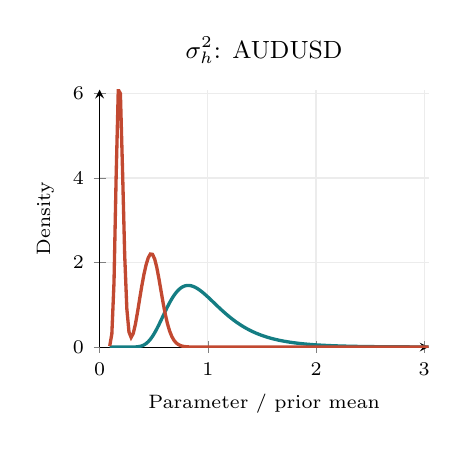
\begin{tikzpicture}
\begin{axis}[width=.475\linewidth,height=4.85cm,title={$\sigma^2_h$: AUDUSD},
 title style={font=\small},xlabel={Parameter / prior mean},ylabel={Density},
 xmin=0,xmax=3.04001,ymin=0,axis lines=left,grid=major,
 grid style={gray!15},tick label style={font=\scriptsize},
 label style={font=\scriptsize},scaled ticks=false]
\addplot[prior,line width=1.2pt,no marks] coordinates {(0.0933371,2.72505e-27) (0.113113,6.90034e-21) (0.13289,1.62751e-16) (0.152666,2.28496e-13) (0.172442,5.16608e-11) (0.192219,3.36135e-09) (0.211995,9.02843e-08) (0.231771,1.26692e-06) (0.251548,1.09e-05) (0.271324,6.43348e-05) (0.2911,0.000282507) (0.310876,0.000979927) (0.330653,0.00280903) (0.350429,0.00688909) (0.370205,0.0148502) (0.389982,0.0287425) (0.409758,0.0508085) (0.429534,0.083166) (0.449311,0.127477) (0.469087,0.184676) (0.488863,0.254809) (0.508639,0.337001) (0.528416,0.429543) (0.548192,0.530063) (0.567968,0.63575) (0.587745,0.743591) (0.607521,0.850585) (0.627297,0.953931) (0.647074,1.05116) (0.66685,1.14022) (0.686626,1.21953) (0.706402,1.28798) (0.726179,1.34491) (0.745955,1.39005) (0.765731,1.42349) (0.785508,1.44562) (0.805284,1.45703) (0.82506,1.4585) (0.844837,1.45093) (0.864613,1.43526) (0.884389,1.41247) (0.904166,1.38356) (0.923942,1.34947) (0.943718,1.31111) (0.963494,1.26934) (0.983271,1.22492) (1.00305,1.17856) (1.02282,1.1309) (1.0426,1.08249) (1.06238,1.03381) (1.08215,0.985297) (1.10193,0.937291) (1.1217,0.890093) (1.14148,0.843945) (1.16126,0.799044) (1.18103,0.755545) (1.20081,0.713565) (1.22059,0.673187) (1.24036,0.63447) (1.26014,0.597445) (1.27992,0.562126) (1.29969,0.528507) (1.31947,0.496572) (1.33924,0.466289) (1.35902,0.43762) (1.3788,0.410518) (1.39857,0.384932) (1.41835,0.360805) (1.43813,0.338079) (1.4579,0.316694) (1.47768,0.296588) (1.49745,0.2777) (1.51723,0.259968) (1.53701,0.243333) (1.55678,0.227735) (1.57656,0.213118) (1.59634,0.199426) (1.61611,0.186605) (1.63589,0.174605) (1.65566,0.163377) (1.67544,0.152874) (1.69522,0.143051) (1.71499,0.133866) (1.73477,0.125279) (1.75455,0.117252) (1.77432,0.10975) (1.7941,0.102739) (1.81388,0.0961875) (1.83365,0.090065) (1.85343,0.0843437) (1.8732,0.0789975) (1.89298,0.0740017) (1.91276,0.069333) (1.93253,0.06497) (1.95231,0.0608922) (1.97209,0.0570808) (1.99186,0.0535181) (2.01164,0.0501874) (2.03141,0.0470733) (2.05119,0.0441614) (2.07097,0.0414383) (2.09074,0.0388912) (2.11052,0.0365085) (2.1303,0.0342792) (2.15007,0.0321931) (2.16985,0.0302406) (2.18963,0.028413) (2.2094,0.0267019) (2.22918,0.0250995) (2.24895,0.0235988) (2.26873,0.0221929) (2.28851,0.0208757) (2.30828,0.0196412) (2.32806,0.018484) (2.34784,0.0173992) (2.36761,0.0163819) (2.38739,0.0154277) (2.40716,0.0145325) (2.42694,0.0136926) (2.44672,0.0129042) (2.46649,0.0121642) (2.48627,0.0114693) (2.50605,0.0108167) (2.52582,0.0102036) (2.5456,0.00962761) (2.56537,0.00908626) (2.58515,0.00857738) (2.60493,0.00809891) (2.6247,0.00764894) (2.64448,0.00722566) (2.66426,0.00682741) (2.68403,0.00645262) (2.70381,0.00609982) (2.72359,0.00576765) (2.74336,0.00545484) (2.76314,0.00516018) (2.78291,0.00488255) (2.80269,0.00462093) (2.82247,0.00437431) (2.84224,0.0041418) (2.86202,0.00392254) (2.8818,0.00371572) (2.90157,0.00352059) (2.92135,0.00333645) (2.94112,0.00316264) (2.9609,0.00299855) (2.98068,0.0028436) (3.00045,0.00269724) (3.02023,0.00255897) (3.04001,0.00242832)};
\addplot[posterior,line width=1.2pt,no marks] coordinates {(0.0933371,0.0249358) (0.113113,0.314874) (0.13289,1.52533) (0.152666,4.03066) (0.172442,6.08851) (0.192219,5.99542) (0.211995,4.1642) (0.231771,2.17059) (0.251548,0.907803) (0.271324,0.356204) (0.2911,0.22868) (0.310876,0.322736) (0.330653,0.540553) (0.350429,0.828411) (0.370205,1.14295) (0.389982,1.44828) (0.409758,1.72097) (0.429534,1.94708) (0.449311,2.11308) (0.469087,2.20106) (0.488863,2.19364) (0.508639,2.0841) (0.528416,1.88312) (0.548192,1.61747) (0.567968,1.32218) (0.587745,1.03087) (0.607521,0.768834) (0.627297,0.550228) (0.647074,0.379079) (0.66685,0.252201) (0.686626,0.162508) (0.706402,0.101696) (0.726179,0.0619607) (0.745955,0.0368391) (0.765731,0.021418) (0.785508,0.0121993) (0.805284,0.00681884) (0.82506,0.00374598) (0.844837,0.00202533) (0.864613,0.00107906) (0.884389,0.00056715) (0.904166,0.000294377) (0.923942,0.000151032) (0.943718,7.66601e-05) (0.963494,3.85252e-05) (0.983271,1.91829e-05) (1.00305,9.47037e-06) (1.02282,4.63851e-06) (1.0426,2.25527e-06) (1.06238,1.0891e-06) (1.08215,5.22634e-07) (1.10193,2.49346e-07) (1.1217,1.18323e-07) (1.14148,5.58706e-08) (1.16126,2.62611e-08) (1.18103,1.22919e-08) (1.20081,5.73128e-09) (1.22059,2.66289e-09) (1.24036,1.23327e-09) (1.26014,5.69496e-10) (1.27992,2.62283e-10) (1.29969,1.20507e-10) (1.31947,5.52481e-11) (1.33924,2.52808e-11) (1.35902,1.15484e-11) (1.3788,5.2675e-12) (1.39857,2.3995e-12) (1.41835,1.09182e-12) (1.43813,4.96326e-13) (1.4579,2.25447e-13) (1.47768,1.0234e-13) (1.49745,4.64344e-14) (1.51723,2.10612e-14) (1.53701,9.55061e-15) (1.55678,4.33051e-15) (1.57656,1.96362e-15) (1.59634,8.90496e-16) (1.61611,4.03933e-16) (1.63589,1.83287e-16) (1.65566,8.32032e-17) (1.67544,3.77895e-17) (1.69522,1.71736e-17) (1.71499,7.80984e-18) (1.73477,3.55426e-18) (1.75455,1.61886e-18) (1.77432,7.37995e-19) (1.7941,3.36749e-19) (1.81388,1.53814e-19) (1.83365,7.03301e-20) (1.85343,3.21936e-20) (1.8732,1.47536e-20) (1.89298,6.76941e-21) (1.91276,3.10988e-21) (1.93253,1.43052e-21) (1.95231,6.58903e-22) (1.97209,3.03905e-22) (1.99186,1.40365e-22) (2.01164,6.49233e-23) (2.03141,3.00728e-23) (2.05119,1.39505e-23) (2.07097,6.4813e-24) (2.09074,3.01578e-24) (2.11052,1.40544e-24) (2.1303,6.5601e-25) (2.15007,3.06692e-25) (2.16985,1.43613e-25) (2.18963,6.73592e-26) (2.2094,3.16457e-26) (2.22918,1.48921e-26) (2.24895,7.01978e-27) (2.26873,3.31456e-27) (2.28851,1.56771e-27) (2.30828,7.42764e-28) (2.32806,3.52519e-28) (2.34784,1.67597e-28) (2.36761,7.98185e-29) (2.38739,3.80802e-29) (2.40716,1.81994e-29) (2.42694,8.71319e-30) (2.44672,4.17892e-30) (2.46649,2.00779e-30) (2.48627,9.66364e-31) (2.50605,4.65945e-31) (2.52582,2.25061e-31) (2.5456,1.08903e-31) (2.56537,5.27902e-32) (2.58515,2.56354e-32) (2.60493,1.2471e-32) (2.6247,6.0777e-33) (2.64448,2.96723e-33) (2.66426,1.45123e-33) (2.68403,7.11047e-34) (2.70381,3.49006e-34) (2.72359,1.7161e-34) (2.74336,8.45324e-35) (2.76314,4.17134e-35) (2.78291,2.06205e-35) (2.80269,1.02116e-35) (2.82247,5.06588e-36) (2.84224,2.51759e-36) (2.86202,1.25337e-36) (2.8818,6.25085e-37) (2.90157,3.12292e-37) (2.92135,1.56295e-37) (2.94112,7.83585e-38) (2.9609,3.93537e-38) (2.98068,1.97989e-38) (3.00045,9.97814e-39) (3.02023,5.03744e-39) (3.04001,2.54753e-39)};
\end{axis}\end{tikzpicture}\hfill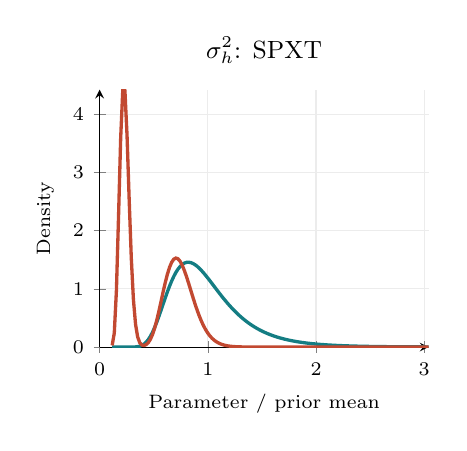
\begin{tikzpicture}
\begin{axis}[width=.475\linewidth,height=4.85cm,title={$\sigma^2_h$: SPXT},
 title style={font=\small},xlabel={Parameter / prior mean},ylabel={Density},
 xmin=0,xmax=3.04001,ymin=0,axis lines=left,grid=major,
 grid style={gray!15},tick label style={font=\scriptsize},
 label style={font=\scriptsize},scaled ticks=false]
\addplot[prior,line width=1.2pt,no marks] coordinates {(0.116073,3.94881e-20) (0.135696,5.24844e-16) (0.15532,5.17641e-13) (0.174944,9.29949e-11) (0.194568,5.17576e-09) (0.214191,1.24575e-07) (0.233815,1.61515e-06) (0.253439,1.31096e-05) (0.273062,7.40716e-05) (0.292686,0.00031465) (0.31231,0.00106395) (0.331934,0.00299019) (0.351557,0.00722105) (0.371181,0.0153784) (0.390805,0.0294822) (0.410428,0.0517259) (0.430052,0.084168) (0.449676,0.128415) (0.4693,0.185362) (0.488923,0.255041) (0.508547,0.336591) (0.528171,0.428342) (0.547794,0.527981) (0.567418,0.632766) (0.587042,0.739755) (0.606666,0.846013) (0.626289,0.948792) (0.645913,1.04566) (0.665537,1.13459) (0.68516,1.21402) (0.704784,1.28281) (0.724408,1.34029) (0.744032,1.38617) (0.763655,1.42052) (0.783279,1.44367) (0.802903,1.4562) (0.822526,1.45884) (0.84215,1.45245) (0.861774,1.43797) (0.881398,1.41634) (0.901021,1.38853) (0.920645,1.35547) (0.940269,1.31807) (0.959892,1.27716) (0.979516,1.23352) (0.99914,1.18784) (1.01876,1.14076) (1.03839,1.09283) (1.05801,1.04456) (1.07763,0.996347) (1.09726,0.948565) (1.11688,0.901514) (1.13651,0.855444) (1.15613,0.810558) (1.17575,0.767016) (1.19538,0.724941) (1.215,0.684425) (1.23462,0.645531) (1.25425,0.608296) (1.27387,0.572738) (1.2935,0.538858) (1.31312,0.506642) (1.33274,0.476064) (1.35237,0.447088) (1.37199,0.419672) (1.39161,0.393766) (1.41124,0.369317) (1.43086,0.346268) (1.45049,0.324561) (1.47011,0.304137) (1.48973,0.284934) (1.50936,0.266894) (1.52898,0.249956) (1.5486,0.234064) (1.56823,0.21916) (1.58785,0.20519) (1.60747,0.192101) (1.6271,0.179841) (1.64672,0.168362) (1.66635,0.157617) (1.68597,0.147562) (1.70559,0.138155) (1.72522,0.129354) (1.74484,0.121124) (1.76446,0.113427) (1.78409,0.106229) (1.80371,0.0994991) (1.82334,0.0932068) (1.84296,0.0873239) (1.86258,0.0818237) (1.88221,0.0766813) (1.90183,0.0718733) (1.92145,0.0673778) (1.94108,0.0631742) (1.9607,0.0592433) (1.98033,0.0555672) (1.99995,0.0521289) (2.01957,0.0489128) (2.0392,0.0459041) (2.05882,0.0430892) (2.07844,0.0404552) (2.09807,0.0379902) (2.11769,0.0356829) (2.13732,0.0335229) (2.15694,0.0315005) (2.17656,0.0296066) (2.19619,0.0278328) (2.21581,0.0261711) (2.23543,0.0246141) (2.25506,0.0231551) (2.27468,0.0217875) (2.2943,0.0205054) (2.31393,0.0193032) (2.33355,0.0181757) (2.35318,0.017118) (2.3728,0.0161256) (2.39242,0.0151943) (2.41205,0.0143202) (2.43167,0.0134995) (2.45129,0.0127288) (2.47092,0.0120049) (2.49054,0.0113248) (2.51017,0.0106858) (2.52979,0.0100852) (2.54941,0.00952056) (2.56904,0.00898964) (2.58866,0.00849031) (2.60828,0.00802057) (2.62791,0.00757859) (2.64753,0.00716261) (2.66716,0.00677104) (2.68678,0.00640234) (2.7064,0.0060551) (2.72603,0.00572801) (2.74565,0.00541983) (2.76527,0.00512939) (2.7849,0.00485561) (2.80452,0.00459748) (2.82415,0.00435405) (2.84377,0.00412442) (2.86339,0.00390778) (2.88302,0.00370334) (2.90264,0.00351037) (2.92226,0.00332818) (2.94189,0.00315613) (2.96151,0.00299363) (2.98113,0.00284011) (3.00076,0.00269505) (3.02038,0.00255794) (3.04001,0.00242832)};
\addplot[posterior,line width=1.2pt,no marks] coordinates {(0.116073,0.0286248) (0.135696,0.243409) (0.15532,0.975053) (0.174944,2.2498) (0.194568,3.59159) (0.214191,4.42401) (0.233815,4.40772) (0.253439,3.63713) (0.273062,2.53887) (0.292686,1.53298) (0.31231,0.8183) (0.331934,0.393996) (0.351557,0.174589) (0.371181,0.0739175) (0.390805,0.0347737) (0.410428,0.0278334) (0.430052,0.0420913) (0.449676,0.0763375) (0.4693,0.133381) (0.488923,0.216344) (0.508547,0.326351) (0.528171,0.461351) (0.547794,0.615939) (0.567418,0.782003) (0.587042,0.949855) (0.606666,1.10951) (0.626289,1.2518) (0.645913,1.36923) (0.665537,1.45642) (0.68516,1.5103) (0.704784,1.53007) (0.724408,1.51693) (0.744032,1.47382) (0.763655,1.40496) (0.783279,1.31543) (0.802903,1.21074) (0.822526,1.09638) (0.84215,0.977542) (0.861774,0.858774) (0.881398,0.743853) (0.901021,0.63569) (0.920645,0.536324) (0.940269,0.446992) (0.959892,0.36823) (0.979516,0.300009) (0.99914,0.241872) (1.01876,0.193065) (1.03839,0.152655) (1.05801,0.119625) (1.07763,0.0929472) (1.09726,0.0716396) (1.11688,0.0547969) (1.13651,0.0416124) (1.15613,0.0313849) (1.17575,0.0235186) (1.19538,0.0175165) (1.215,0.0129709) (1.23462,0.00955258) (1.25425,0.00699886) (1.27387,0.00510287) (1.2935,0.00370338) (1.31312,0.00267603) (1.33274,0.00192573) (1.35237,0.00138043) (1.37199,0.000985924) (1.39161,0.000701729) (1.41124,0.000497828) (1.43086,0.00035209) (1.45049,0.000248295) (1.47011,0.000174622) (1.48973,0.000122493) (1.50936,8.57183e-05) (1.52898,5.98477e-05) (1.5486,4.16958e-05) (1.56823,2.89911e-05) (1.58785,2.01195e-05) (1.60747,1.39381e-05) (1.6271,9.63982e-06) (1.64672,6.65673e-06) (1.66635,4.59011e-06) (1.68597,3.16081e-06) (1.70559,2.17383e-06) (1.72522,1.49328e-06) (1.74484,1.02467e-06) (1.76446,7.02405e-07) (1.78409,4.81043e-07) (1.80371,3.29158e-07) (1.82334,2.25051e-07) (1.84296,1.53758e-07) (1.86258,1.0498e-07) (1.88221,7.16322e-08) (1.90183,4.88508e-08) (1.92145,3.32981e-08) (1.94108,2.26868e-08) (1.9607,1.5451e-08) (1.98033,1.05193e-08) (1.99995,7.15952e-09) (2.01957,4.87157e-09) (2.0392,3.31405e-09) (2.05882,2.25409e-09) (2.07844,1.53292e-09) (2.09807,1.04237e-09) (2.11769,7.08755e-10) (2.13732,4.81894e-10) (2.15694,3.27645e-10) (2.17656,2.22774e-10) (2.19619,1.51477e-10) (2.21581,1.03007e-10) (2.23543,7.00534e-11) (2.25506,4.76485e-11) (2.27468,3.24143e-11) (2.2943,2.20546e-11) (2.31393,1.50089e-11) (2.33355,1.02164e-11) (2.35318,6.95579e-12) (2.3728,4.73707e-12) (2.39242,3.22696e-12) (2.41205,2.1989e-12) (2.43167,1.49884e-12) (2.45129,1.02199e-12) (2.47092,6.97085e-13) (2.49054,4.75644e-13) (2.51017,3.24669e-13) (2.52979,2.21701e-13) (2.54941,1.51449e-13) (2.56904,1.03501e-13) (2.58866,7.07634e-14) (2.60828,4.84017e-14) (2.62791,3.31212e-14) (2.64753,2.26751e-14) (2.66716,1.55308e-14) (2.68678,1.06426e-14) (2.7064,7.2964e-15) (2.72603,5.00478e-15) (2.74565,3.43462e-15) (2.76527,2.35827e-15) (2.7849,1.62006e-15) (2.80452,1.11352e-15) (2.82415,7.6576e-16) (2.84377,5.26891e-16) (2.86339,3.62731e-16) (2.88302,2.49854e-16) (2.90264,1.72198e-16) (2.92226,1.18744e-16) (2.94189,8.19299e-17) (2.96151,5.65612e-17) (2.98113,3.907e-17) (3.00076,2.70034e-17) (3.02038,1.86744e-17) (3.04001,1.29219e-17)};
\end{axis}\end{tikzpicture}
\par\smallskip
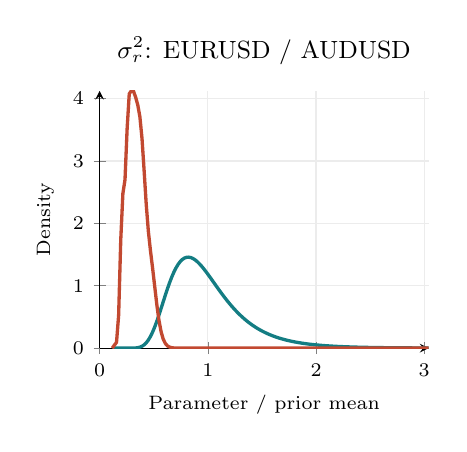
\begin{tikzpicture}
\begin{axis}[width=.475\linewidth,height=4.85cm,title={$\sigma^2_r$: EURUSD / AUDUSD},
 title style={font=\small},xlabel={Parameter / prior mean},ylabel={Density},
 xmin=0,xmax=3.04001,ymin=0,axis lines=left,grid=major,
 grid style={gray!15},tick label style={font=\scriptsize},
 label style={font=\scriptsize},scaled ticks=false]
\addplot[prior,line width=1.2pt,no marks] coordinates {(0.116929,6.42615e-20) (0.136547,7.40625e-16) (0.156165,6.67187e-13) (0.175783,1.12783e-10) (0.195401,6.01488e-09) (0.215019,1.40359e-07) (0.234637,1.77829e-06) (0.254255,1.41818e-05) (0.273873,7.90401e-05) (0.293491,0.000332142) (0.313109,0.00111339) (0.332727,0.00310717) (0.352345,0.00746032) (0.371963,0.015812) (0.39158,0.0301927) (0.411198,0.0527944) (0.430816,0.0856621) (0.450434,0.130377) (0.470052,0.187803) (0.48967,0.257936) (0.509288,0.339884) (0.528906,0.43195) (0.548524,0.531803) (0.568142,0.636693) (0.58776,0.743675) (0.607378,0.849822) (0.626996,0.952397) (0.646614,1.04898) (0.666232,1.13758) (0.68585,1.21662) (0.705468,1.285) (0.725086,1.34207) (0.744704,1.38754) (0.764322,1.42149) (0.78394,1.44426) (0.803558,1.45644) (0.823176,1.45877) (0.842794,1.4521) (0.862412,1.43737) (0.88203,1.41553) (0.901648,1.38755) (0.921266,1.35435) (0.940884,1.31684) (0.960502,1.27585) (0.98012,1.23214) (0.999737,1.18642) (1.01936,1.13932) (1.03897,1.0914) (1.05859,1.04313) (1.07821,0.99494) (1.09783,0.94719) (1.11745,0.900178) (1.13706,0.854152) (1.15668,0.809315) (1.1763,0.765825) (1.19592,0.723805) (1.21554,0.683344) (1.23515,0.644505) (1.25477,0.607326) (1.27439,0.571823) (1.29401,0.537997) (1.31362,0.505834) (1.33324,0.475306) (1.35286,0.446379) (1.37248,0.419009) (1.3921,0.393147) (1.41171,0.36874) (1.43133,0.345731) (1.45095,0.324062) (1.47057,0.303673) (1.49019,0.284504) (1.5098,0.266495) (1.52942,0.249587) (1.54904,0.233722) (1.56866,0.218844) (1.58828,0.204897) (1.60789,0.19183) (1.62751,0.179591) (1.64713,0.168131) (1.66675,0.157404) (1.68637,0.147366) (1.70598,0.137974) (1.7256,0.129188) (1.74522,0.12097) (1.76484,0.113285) (1.78446,0.106099) (1.80407,0.0993792) (1.82369,0.0930965) (1.84331,0.0872224) (1.86293,0.0817303) (1.88255,0.0765954) (1.90216,0.0717944) (1.92178,0.0673053) (1.9414,0.0631076) (1.96102,0.0591821) (1.98064,0.055511) (2.00025,0.0520773) (2.01987,0.0488655) (2.03949,0.0458607) (2.05911,0.0430494) (2.07873,0.0404187) (2.09834,0.0379567) (2.11796,0.0356521) (2.13758,0.0334947) (2.1572,0.0314747) (2.17682,0.029583) (2.19643,0.0278112) (2.21605,0.0261513) (2.23567,0.0245961) (2.25529,0.0231385) (2.27491,0.0217724) (2.29452,0.0204916) (2.31414,0.0192906) (2.33376,0.0181642) (2.35338,0.0171075) (2.373,0.0161161) (2.39261,0.0151856) (2.41223,0.0143122) (2.43185,0.0134922) (2.45147,0.0127222) (2.47109,0.0119989) (2.4907,0.0113194) (2.51032,0.0106809) (2.52994,0.0100808) (2.54956,0.00951656) (2.56917,0.00898603) (2.58879,0.00848705) (2.60841,0.00801764) (2.62803,0.00757595) (2.64765,0.00716025) (2.66726,0.00676892) (2.68688,0.00640045) (2.7065,0.00605343) (2.72612,0.00572653) (2.74574,0.00541851) (2.76535,0.00512823) (2.78497,0.0048546) (2.80459,0.0045966) (2.82421,0.00435328) (2.84383,0.00412377) (2.86344,0.00390723) (2.88306,0.00370287) (2.90268,0.00350998) (2.9223,0.00332787) (2.94192,0.00315589) (2.96153,0.00299345) (2.98115,0.00283998) (3.00077,0.00269496) (3.02039,0.0025579) (3.04001,0.00242832)};
\addplot[posterior,line width=1.2pt,no marks] coordinates {(0.116929,0.000261163) (0.136547,0.0484096) (0.156165,0.0925754) (0.175783,0.528563) (0.195401,1.74093) (0.215019,2.47875) (0.234637,2.70094) (0.254255,3.52037) (0.273873,4.07799) (0.293491,4.12622) (0.313109,4.11897) (0.332727,4.02364) (0.352345,3.90038) (0.371963,3.71126) (0.39158,3.36433) (0.411198,2.84765) (0.430816,2.30397) (0.450434,1.87385) (0.470052,1.55973) (0.48967,1.28161) (0.509288,0.98672) (0.528906,0.692685) (0.548524,0.444095) (0.568142,0.26303) (0.58776,0.144965) (0.607378,0.0746983) (0.626996,0.0363011) (0.646614,0.0167901) (0.666232,0.00738369) (0.68585,0.00304345) (0.705468,0.00115315) (0.725086,0.000395524) (0.744704,0.000121847) (0.764322,3.36658e-05) (0.78394,8.36506e-06) (0.803558,1.87847e-06) (0.823176,3.83522e-07) (0.842794,7.16405e-08) (0.862412,1.23201e-08) (0.88203,1.96227e-09) (0.901648,2.91097e-10) (0.921266,4.04334e-11) (0.940884,5.2844e-12) (0.960502,6.52795e-13) (0.98012,7.65441e-14) (0.999737,8.55245e-15) (1.01936,9.13859e-16) (1.03897,9.36975e-17) (1.05859,9.24655e-18) (1.07821,8.80808e-19) (1.09783,8.1206e-20) (1.11745,7.264e-21) (1.13706,6.31891e-22) (1.15668,5.35694e-23) (1.1763,4.4347e-24) (1.19592,3.59164e-25) (1.21554,2.85071e-26) (1.23515,2.221e-27) (1.25477,1.70111e-28) (1.27439,1.28268e-29) (1.29401,9.53417e-31) (1.31362,6.99453e-32) (1.33324,5.07047e-33) (1.35286,3.636e-34) (1.37248,2.58181e-35) (1.3921,1.81704e-36) (1.41171,1.26863e-37) (1.43133,8.7942e-39) (1.45095,6.05749e-40) (1.47057,4.14903e-41) (1.49019,2.82786e-42) (1.5098,1.91917e-43) (1.52942,1.29772e-44) (1.54904,8.748e-46) (1.56866,5.88216e-47) (1.58828,3.94718e-48) (1.60789,2.64466e-49) (1.62751,1.77004e-50) (1.64713,1.18389e-51) (1.66675,7.91651e-53) (1.68637,5.29436e-54) (1.70598,3.54248e-55) (1.7256,2.37226e-56) (1.74522,1.59044e-57) (1.76484,1.06783e-58) (1.78446,7.18193e-60) (1.80407,4.84006e-61) (1.82369,3.26919e-62) (1.84331,2.21367e-63) (1.86293,1.50303e-64) (1.88255,1.02351e-65) (1.90216,6.99166e-67) (1.92178,4.79191e-68) (1.9414,3.29575e-69) (1.96102,2.27505e-70) (1.98064,1.57648e-71) (2.00025,1.09675e-72) (2.01987,7.66147e-74) (2.03949,5.37474e-75) (2.05911,3.78702e-76) (2.07873,2.6803e-77) (2.09834,1.90573e-78) (2.11796,1.36137e-79) (2.13758,9.77172e-81) (2.1572,7.04829e-82) (2.17682,5.10918e-83) (2.19643,3.72227e-84) (2.21605,2.72576e-85) (2.23567,2.0064e-86) (2.25529,1.48466e-87) (2.27491,1.10444e-88) (2.29452,8.26019e-90) (2.31414,6.2114e-91) (2.33376,4.69638e-92) (2.35338,3.57052e-93) (2.373,2.72967e-94) (2.39261,2.09855e-95) (2.41223,1.62245e-96) (2.43185,1.26148e-97) (2.45147,9.86418e-99) (2.47109,7.75755e-100) (2.4907,6.13594e-101) (2.51032,4.88136e-102) (2.52994,3.90582e-103) (2.54956,3.14342e-104) (2.56917,2.5446e-105) (2.58879,2.07189e-106) (2.60841,1.69689e-107) (2.62803,1.39792e-108) (2.64765,1.15839e-109) (2.66726,9.65553e-111) (2.68688,8.0956e-112) (2.7065,6.82769e-113) (2.72612,5.79232e-114) (2.74574,4.94294e-115) (2.76535,4.24299e-116) (2.78497,3.66364e-117) (2.80459,3.18204e-118) (2.82421,2.78003e-119) (2.84383,2.44312e-120) (2.86344,2.15966e-121) (2.88306,1.92031e-122) (2.90268,1.7175e-123) (2.9223,1.54512e-124) (2.94192,1.39817e-125) (2.96153,1.27259e-126) (2.98115,1.16504e-127) (3.00077,1.07279e-128) (3.02039,9.93587e-130) (3.04001,9.25564e-131)};
\end{axis}\end{tikzpicture}\hfill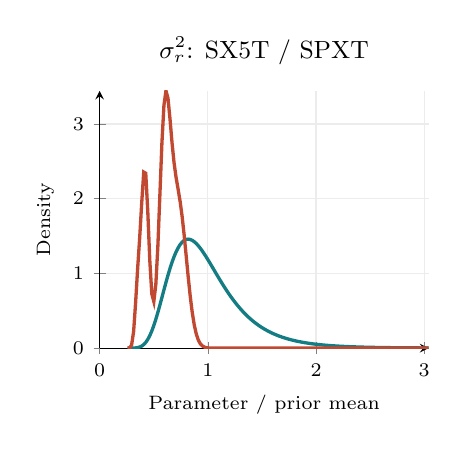
\begin{tikzpicture}
\begin{axis}[width=.475\linewidth,height=4.85cm,title={$\sigma^2_r$: SX5T / SPXT},
 title style={font=\small},xlabel={Parameter / prior mean},ylabel={Density},
 xmin=0,xmax=3.04001,ymin=0,axis lines=left,grid=major,
 grid style={gray!15},tick label style={font=\scriptsize},
 label style={font=\scriptsize},scaled ticks=false]
\addplot[prior,line width=1.2pt,no marks] coordinates {(0.258302,2.07563e-05) (0.276971,0.000100868) (0.29564,0.000383079) (0.314309,0.00119137) (0.332978,0.0031451) (0.351648,0.00724816) (0.370317,0.0149097) (0.388986,0.0278663) (0.407655,0.0480074) (0.426324,0.0771371) (0.444993,0.116723) (0.463662,0.167684) (0.482332,0.230251) (0.501001,0.303917) (0.51967,0.38748) (0.538339,0.479153) (0.557008,0.576717) (0.575677,0.677699) (0.594347,0.779547) (0.613016,0.879778) (0.631685,0.976109) (0.650354,1.06654) (0.669023,1.14944) (0.687692,1.22351) (0.706361,1.28785) (0.725031,1.34192) (0.7437,1.38549) (0.762369,1.41862) (0.781038,1.44158) (0.799707,1.45485) (0.818376,1.45906) (0.837046,1.45493) (0.855715,1.44325) (0.874384,1.42483) (0.893053,1.4005) (0.911722,1.37109) (0.930391,1.33739) (0.949061,1.30013) (0.96773,1.26002) (0.986399,1.21769) (1.00507,1.17374) (1.02374,1.12867) (1.04241,1.08296) (1.06108,1.03701) (1.07974,0.991183) (1.09841,0.945772) (1.11708,0.901038) (1.13575,0.857193) (1.15442,0.814414) (1.17309,0.77284) (1.19176,0.732582) (1.21043,0.693722) (1.2291,0.656318) (1.24777,0.620408) (1.26644,0.586013) (1.28511,0.553139) (1.30377,0.521777) (1.32244,0.49191) (1.34111,0.463512) (1.35978,0.436548) (1.37845,0.410979) (1.39712,0.386761) (1.41579,0.363848) (1.43446,0.34219) (1.45313,0.321737) (1.4718,0.302438) (1.49047,0.284239) (1.50914,0.267091) (1.5278,0.250941) (1.54647,0.235741) (1.56514,0.22144) (1.58381,0.207992) (1.60248,0.195351) (1.62115,0.183473) (1.63982,0.172314) (1.65849,0.161834) (1.67716,0.151995) (1.69583,0.142758) (1.7145,0.134089) (1.73317,0.125954) (1.75183,0.118321) (1.7705,0.11116) (1.78917,0.104442) (1.80784,0.0981396) (1.82651,0.0922279) (1.84518,0.0866828) (1.86385,0.0814814) (1.88252,0.0766024) (1.90119,0.0720258) (1.91986,0.0677326) (1.93853,0.0637051) (1.9572,0.0599266) (1.97586,0.0563815) (1.99453,0.053055) (2.0132,0.0499334) (2.03187,0.0470038) (2.05054,0.0442541) (2.06921,0.0416729) (2.08788,0.0392497) (2.10655,0.0369743) (2.12522,0.0348376) (2.14389,0.0328308) (2.16256,0.0309457) (2.18122,0.0291746) (2.19989,0.0275105) (2.21856,0.0259465) (2.23723,0.0244764) (2.2559,0.0230944) (2.27457,0.021795) (2.29324,0.0205729) (2.31191,0.0194234) (2.33058,0.018342) (2.34925,0.0173244) (2.36792,0.0163667) (2.38659,0.0154652) (2.40525,0.0146165) (2.42392,0.0138173) (2.44259,0.0130645) (2.46126,0.0123554) (2.47993,0.0116873) (2.4986,0.0110576) (2.51727,0.0104641) (2.53594,0.0099045) (2.55461,0.00937683) (2.57328,0.00887914) (2.59195,0.00840965) (2.61062,0.00796665) (2.62928,0.00754858) (2.64795,0.00715394) (2.66662,0.00678135) (2.68529,0.00642951) (2.70396,0.00609719) (2.72263,0.00578324) (2.7413,0.00548658) (2.75997,0.00520622) (2.77864,0.0049412) (2.79731,0.00469062) (2.81598,0.00445365) (2.83465,0.00422952) (2.85331,0.00401747) (2.87198,0.00381682) (2.89065,0.00362692) (2.90932,0.00344715) (2.92799,0.00327694) (2.94666,0.00311576) (2.96533,0.00296308) (2.984,0.00281843) (3.00267,0.00268137) (3.02134,0.00255146) (3.04001,0.00242832)};
\addplot[posterior,line width=1.2pt,no marks] coordinates {(0.258302,6.1211e-05) (0.276971,0.00295656) (0.29564,0.0411158) (0.314309,0.223816) (0.332978,0.616822) (0.351648,1.07154) (0.370317,1.47791) (0.388986,1.94389) (0.407655,2.35689) (0.426324,2.34099) (0.444993,1.83167) (0.463662,1.17362) (0.482332,0.725004) (0.501001,0.624077) (0.51967,0.857291) (0.538339,1.36804) (0.557008,2.05485) (0.575677,2.746) (0.594347,3.24894) (0.613016,3.44531) (0.631685,3.34669) (0.650354,3.06883) (0.669023,2.75105) (0.687692,2.48405) (0.706361,2.28723) (0.725031,2.12967) (0.7437,1.96584) (0.762369,1.76367) (0.781038,1.51622) (0.799707,1.23866) (0.818376,0.957404) (0.837046,0.698621) (0.855715,0.480682) (0.874384,0.311573) (0.893053,0.190119) (0.911722,0.109144) (0.930391,0.0589295) (0.949061,0.0299244) (0.96773,0.0142969) (0.986399,0.00643158) (1.00507,0.00272728) (1.02374,0.00109164) (1.04241,0.000413107) (1.06108,0.000148058) (1.07974,5.03489e-05) (1.09841,1.62764e-05) (1.11708,5.01146e-06) (1.13575,1.47244e-06) (1.15442,4.13609e-07) (1.17309,1.11282e-07) (1.19176,2.87293e-08) (1.21043,7.12927e-09) (1.2291,1.70342e-09) (1.24777,3.92524e-10) (1.26644,8.73706e-11) (1.28511,1.8814e-11) (1.30377,3.92514e-12) (1.32244,7.94509e-13) (1.34111,1.56244e-13) (1.35978,2.9891e-14) (1.37845,5.56998e-15) (1.39712,1.0122e-15) (1.41579,1.79592e-16) (1.43446,3.11454e-17) (1.45313,5.2851e-18) (1.4718,8.78433e-19) (1.49047,1.43148e-19) (1.50914,2.28925e-20) (1.5278,3.59603e-21) (1.54647,5.55329e-22) (1.56514,8.43788e-23) (1.58381,1.26246e-23) (1.60248,1.86136e-24) (1.62115,2.70639e-25) (1.63982,3.88327e-26) (1.65849,5.50228e-27) (1.67716,7.70378e-28) (1.69583,1.06646e-28) (1.7145,1.46058e-29) (1.73317,1.98008e-30) (1.75183,2.65862e-31) (1.7705,3.53726e-32) (1.78917,4.66584e-33) (1.80784,6.10451e-34) (1.82651,7.92553e-35) (1.84518,1.02153e-35) (1.86385,1.30767e-36) (1.88252,1.66321e-37) (1.90119,2.10262e-38) (1.91986,2.64303e-39) (1.93853,3.30463e-40) (1.9572,4.11123e-41) (1.97586,5.09084e-42) (1.99453,6.2764e-43) (2.0132,7.70665e-44) (2.03187,9.42714e-45) (2.05054,1.14914e-45) (2.06921,1.39624e-46) (2.08788,1.69143e-47) (2.10655,2.04342e-48) (2.12522,2.46248e-49) (2.14389,2.96074e-50) (2.16256,3.55248e-51) (2.18122,4.2546e-52) (2.19989,5.08709e-53) (2.21856,6.07358e-54) (2.23723,7.24214e-55) (2.2559,8.62606e-56) (2.27457,1.02649e-56) (2.29324,1.22058e-57) (2.31191,1.4505e-58) (2.33058,1.72294e-59) (2.34925,2.04593e-60) (2.36792,2.42906e-61) (2.38659,2.88385e-62) (2.40525,3.42413e-63) (2.42392,4.06653e-64) (2.44259,4.83112e-65) (2.46126,5.74211e-66) (2.47993,6.82876e-67) (2.4986,8.12657e-68) (2.51727,9.67857e-69) (2.53594,1.15371e-69) (2.55461,1.37659e-70) (2.57328,1.64429e-71) (2.59195,1.96631e-72) (2.61062,2.3543e-73) (2.62928,2.82258e-74) (2.64795,3.38874e-75) (2.66662,4.07446e-76) (2.68529,4.90651e-77) (2.70396,5.91804e-78) (2.72263,7.15013e-79) (2.7413,8.65384e-80) (2.75997,1.04928e-80) (2.77864,1.27462e-81) (2.79731,1.55135e-82) (2.81598,1.89191e-83) (2.83465,2.31192e-84) (2.85331,2.83107e-85) (2.87198,3.4742e-86) (2.89065,4.27275e-87) (2.90932,5.26654e-88) (2.92799,6.50623e-89) (2.94666,8.05632e-90) (2.96533,9.99919e-91) (2.984,1.24403e-91) (3.00267,1.55149e-92) (3.02134,1.9397e-93) (3.04001,2.43112e-94)};
\end{axis}\end{tikzpicture}
\par\smallskip
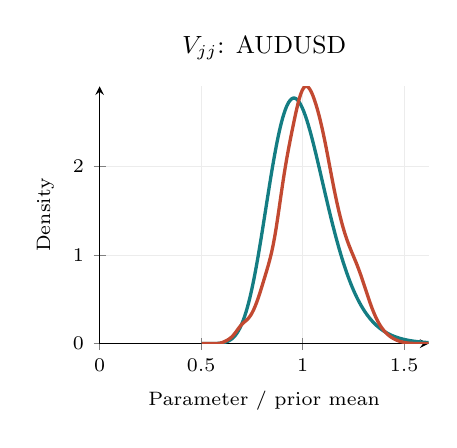
\begin{tikzpicture}
\begin{axis}[width=.475\linewidth,height=4.85cm,title={$V_{jj}$: AUDUSD},
 title style={font=\small},xlabel={Parameter / prior mean},ylabel={Density},
 xmin=0,xmax=1.62036,ymin=0,axis lines=left,grid=major,
 grid style={gray!15},tick label style={font=\scriptsize},
 label style={font=\scriptsize},scaled ticks=false]
\addplot[prior,line width=1.2pt,no marks] coordinates {(0.502927,1.59643e-05) (0.510427,2.94329e-05) (0.517926,5.27869e-05) (0.525426,9.22153e-05) (0.532925,0.00015711) (0.540425,0.000261361) (0.547924,0.000425001) (0.555424,0.000676245) (0.562923,0.00105393) (0.570423,0.00161033) (0.577922,0.00241431) (0.585422,0.00355475) (0.592922,0.00514402) (0.600421,0.00732143) (0.607921,0.0102564) (0.61542,0.0141511) (0.62292,0.0192423) (0.630419,0.0258021) (0.637919,0.0341377) (0.645418,0.0445891) (0.652918,0.0575259) (0.660417,0.0733417) (0.667917,0.0924474) (0.675416,0.115263) (0.682916,0.142205) (0.690416,0.17368) (0.697915,0.21007) (0.705415,0.251717) (0.712914,0.298916) (0.720414,0.351902) (0.727913,0.410835) (0.735413,0.475796) (0.742912,0.546773) (0.750412,0.623661) (0.757911,0.706257) (0.765411,0.794256) (0.77291,0.887256) (0.78041,0.984758) (0.78791,1.08618) (0.795409,1.19085) (0.802909,1.29804) (0.810408,1.40696) (0.817908,1.51677) (0.825407,1.62661) (0.832907,1.73559) (0.840406,1.84283) (0.847906,1.94746) (0.855405,2.04864) (0.862905,2.14556) (0.870404,2.23748) (0.877904,2.32369) (0.885403,2.40359) (0.892903,2.47661) (0.900403,2.54229) (0.907902,2.60025) (0.915402,2.6502) (0.922901,2.69193) (0.930401,2.72532) (0.9379,2.75032) (0.9454,2.76697) (0.952899,2.77539) (0.960399,2.77576) (0.967898,2.76833) (0.975398,2.75339) (0.982897,2.73129) (0.990397,2.70244) (0.997897,2.66724) (1.0054,2.62617) (1.0129,2.57969) (1.0204,2.52829) (1.02789,2.47247) (1.03539,2.41273) (1.04289,2.34957) (1.05039,2.28346) (1.05789,2.2149) (1.06539,2.14433) (1.07289,2.07221) (1.08039,1.99894) (1.08789,1.92494) (1.09539,1.85057) (1.10289,1.77618) (1.11039,1.70208) (1.11789,1.62857) (1.12539,1.55592) (1.13289,1.48436) (1.14039,1.4141) (1.14789,1.34533) (1.15539,1.27821) (1.16289,1.21287) (1.17039,1.14944) (1.17789,1.08801) (1.18538,1.02865) (1.19288,0.97141) (1.20038,0.91634) (1.20788,0.86346) (1.21538,0.812779) (1.22288,0.764295) (1.23038,0.717993) (1.23788,0.673849) (1.24538,0.631829) (1.25288,0.591894) (1.26038,0.553996) (1.26788,0.518081) (1.27538,0.484094) (1.28288,0.451972) (1.29038,0.421651) (1.29788,0.393066) (1.30538,0.36615) (1.31288,0.340832) (1.32038,0.317044) (1.32788,0.294718) (1.33538,0.273785) (1.34288,0.254177) (1.35037,0.235828) (1.35787,0.218673) (1.36537,0.202647) (1.37287,0.187691) (1.38037,0.173743) (1.38787,0.160746) (1.39537,0.148645) (1.40287,0.137387) (1.41037,0.126919) (1.41787,0.117194) (1.42537,0.108165) (1.43287,0.099788) (1.44037,0.09202) (1.44787,0.0848216) (1.45537,0.0781549) (1.46287,0.0719841) (1.47037,0.0662756) (1.47787,0.0609975) (1.48537,0.0561199) (1.49287,0.0516147) (1.50037,0.0474555) (1.50787,0.0436174) (1.51536,0.0400773) (1.52286,0.0368136) (1.53036,0.0338058) (1.53786,0.0310351) (1.54536,0.0284837) (1.55286,0.0261353) (1.56036,0.0239744) (1.56786,0.0219869) (1.57536,0.0201594) (1.58286,0.0184796) (1.59036,0.016936) (1.59786,0.0155182) (1.60536,0.0142161) (1.61286,0.0130208) (1.62036,0.0119237)};
\addplot[posterior,line width=1.2pt,no marks] coordinates {(0.502927,3.39529e-11) (0.510427,4.56503e-10) (0.517926,4.96023e-09) (0.525426,4.39393e-08) (0.532925,3.19992e-07) (0.540425,1.93134e-06) (0.547924,9.73633e-06) (0.555424,4.13105e-05) (0.562923,0.000148639) (0.570423,0.000457005) (0.577922,0.00121019) (0.585422,0.00278359) (0.592922,0.00561381) (0.600421,0.0100356) (0.607921,0.0161117) (0.61542,0.0236039) (0.62292,0.0321675) (0.630419,0.0416763) (0.637919,0.0524535) (0.645418,0.0652248) (0.652918,0.0807889) (0.660417,0.0995724) (0.667917,0.121293) (0.675416,0.144898) (0.682916,0.16882) (0.690416,0.191447) (0.697915,0.211637) (0.705415,0.229083) (0.712914,0.244419) (0.720414,0.259064) (0.727913,0.274873) (0.735413,0.293703) (0.742912,0.317021) (0.750412,0.34567) (0.757911,0.379834) (0.765411,0.419208) (0.77291,0.463235) (0.78041,0.511293) (0.78791,0.562729) (0.795409,0.616793) (0.802909,0.67261) (0.810408,0.72932) (0.817908,0.786448) (0.825407,0.84433) (0.832907,0.904389) (0.840406,0.969024) (0.847906,1.04107) (0.855405,1.123) (0.862905,1.21613) (0.870404,1.32012) (0.877904,1.43295) (0.885403,1.55131) (0.892903,1.67127) (0.900403,1.78913) (0.907902,1.902) (0.915402,2.0083) (0.922901,2.10781) (0.930401,2.20146) (0.9379,2.29079) (0.9454,2.37735) (0.952899,2.46209) (0.960399,2.54493) (0.967898,2.62463) (0.975398,2.69901) (0.982897,2.76537) (0.990397,2.82109) (0.997897,2.86411) (1.0054,2.89322) (1.0129,2.90816) (1.0204,2.9095) (1.02789,2.89837) (1.03539,2.8762) (1.04289,2.84451) (1.05039,2.8047) (1.05789,2.75792) (1.06539,2.70503) (1.07289,2.6466) (1.08039,2.58288) (1.08789,2.51397) (1.09539,2.43994) (1.10289,2.36098) (1.11039,2.27754) (1.11789,2.19041) (1.12539,2.10065) (1.13289,2.00959) (1.14039,1.91859) (1.14789,1.82897) (1.15539,1.74184) (1.16289,1.65804) (1.17039,1.57818) (1.17789,1.50262) (1.18538,1.43159) (1.19288,1.3652) (1.20038,1.30348) (1.20788,1.24636) (1.21538,1.19363) (1.22288,1.14488) (1.23038,1.09949) (1.23788,1.05662) (1.24538,1.01528) (1.25288,0.974405) (1.26038,0.932971) (1.26788,0.89013) (1.27538,0.845296) (1.28288,0.798207) (1.29038,0.748935) (1.29788,0.69786) (1.30538,0.645602) (1.31288,0.592935) (1.32038,0.540698) (1.32788,0.489713) (1.33538,0.440719) (1.34288,0.394323) (1.35037,0.350977) (1.35787,0.310974) (1.36537,0.274448) (1.37287,0.241403) (1.38037,0.211728) (1.38787,0.185232) (1.39537,0.161667) (1.40287,0.140757) (1.41037,0.12222) (1.41787,0.105784) (1.42537,0.0912015) (1.43287,0.0782566) (1.44037,0.0667669) (1.44787,0.0565824) (1.45537,0.047581) (1.46287,0.0396628) (1.47037,0.0327431) (1.47787,0.0267466) (1.48537,0.0216018) (1.49287,0.0172382) (1.50037,0.0135836) (1.50787,0.0105644) (1.51536,0.00810595) (1.52286,0.006134) (1.53036,0.00457666) (1.53786,0.00336611) (1.54536,0.00244013) (1.55286,0.00174323) (1.56036,0.00122722) (1.56786,0.000851338) (1.57536,0.000581953) (1.58286,0.000392002) (1.59036,0.000260208) (1.59786,0.000170219) (1.60536,0.000109745) (1.61286,6.9741e-05) (1.62036,4.36877e-05)};
\end{axis}\end{tikzpicture}\hfill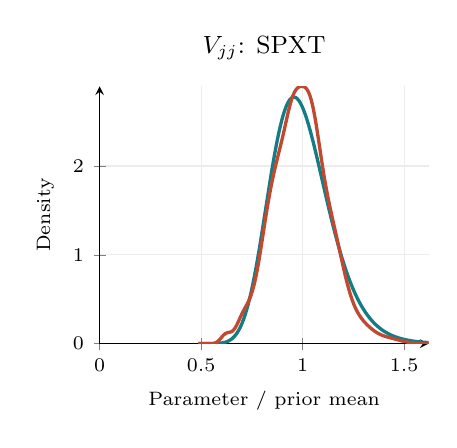
\begin{tikzpicture}
\begin{axis}[width=.475\linewidth,height=4.85cm,title={$V_{jj}$: SPXT},
 title style={font=\small},xlabel={Parameter / prior mean},ylabel={Density},
 xmin=0,xmax=1.62036,ymin=0,axis lines=left,grid=major,
 grid style={gray!15},tick label style={font=\scriptsize},
 label style={font=\scriptsize},scaled ticks=false]
\addplot[prior,line width=1.2pt,no marks] coordinates {(0.486753,3.85818e-06) (0.494361,7.6597e-06) (0.501969,1.47334e-05) (0.509577,2.75005e-05) (0.517185,4.98848e-05) (0.524793,8.80624e-05) (0.532401,0.000151487) (0.540009,0.000254246) (0.547617,0.000416805) (0.555225,0.000668165) (0.562833,0.00104846) (0.570442,0.00161199) (0.57805,0.00243057) (0.585658,0.00359722) (0.593266,0.00522992) (0.600874,0.00747529) (0.608482,0.010512) (0.61609,0.0145535) (0.623698,0.01985) (0.631306,0.0266891) (0.638914,0.0353956) (0.646522,0.0463286) (0.654131,0.0598776) (0.661739,0.0764571) (0.669347,0.0964982) (0.676955,0.120439) (0.684563,0.148715) (0.692171,0.181745) (0.699779,0.219918) (0.707387,0.263583) (0.714995,0.313032) (0.722603,0.36849) (0.730211,0.430101) (0.73782,0.497922) (0.745428,0.571911) (0.753036,0.651924) (0.760644,0.737714) (0.768252,0.828924) (0.77586,0.925097) (0.783468,1.02568) (0.791076,1.13002) (0.798684,1.2374) (0.806292,1.34702) (0.8139,1.45804) (0.821509,1.56956) (0.829117,1.68067) (0.836725,1.79046) (0.844333,1.89799) (0.851941,2.00238) (0.859549,2.10277) (0.867157,2.19834) (0.874765,2.28835) (0.882373,2.3721) (0.889981,2.44901) (0.897589,2.51854) (0.905198,2.58026) (0.912806,2.63384) (0.920414,2.67901) (0.928022,2.71564) (0.93563,2.74363) (0.943238,2.76302) (0.950846,2.77389) (0.958454,2.77643) (0.966062,2.77085) (0.97367,2.75748) (0.981278,2.73665) (0.988887,2.70877) (0.996495,2.67428) (1.0041,2.63365) (1.01171,2.58737) (1.01932,2.53595) (1.02693,2.47991) (1.03454,2.41976) (1.04214,2.35603) (1.04975,2.28922) (1.05736,2.21985) (1.06497,2.14837) (1.07258,2.07527) (1.08018,2.00099) (1.08779,1.92592) (1.0954,1.85048) (1.10301,1.77501) (1.11062,1.69985) (1.11822,1.62531) (1.12583,1.55165) (1.13344,1.47914) (1.14105,1.40798) (1.14866,1.33836) (1.15626,1.27046) (1.16387,1.20442) (1.17148,1.14035) (1.17909,1.07834) (1.1867,1.01848) (1.19431,0.960812) (1.20191,0.90538) (1.20952,0.852206) (1.21713,0.801295) (1.22474,0.752642) (1.23235,0.706229) (1.23995,0.662029) (1.24756,0.620006) (1.25517,0.580113) (1.26278,0.542301) (1.27039,0.506512) (1.27799,0.472686) (1.2856,0.440757) (1.29321,0.410658) (1.30082,0.382318) (1.30843,0.355668) (1.31603,0.330635) (1.32364,0.307146) (1.33125,0.285131) (1.33886,0.264518) (1.34647,0.245237) (1.35407,0.227219) (1.36168,0.210397) (1.36929,0.194706) (1.3769,0.180082) (1.38451,0.166464) (1.39212,0.153793) (1.39972,0.142013) (1.40733,0.131069) (1.41494,0.12091) (1.42255,0.111485) (1.43016,0.102747) (1.43776,0.094652) (1.44537,0.0871572) (1.45298,0.0802224) (1.46059,0.0738094) (1.4682,0.0678826) (1.4758,0.0624079) (1.48341,0.0573538) (1.49102,0.0526903) (1.49863,0.0483893) (1.50624,0.0444246) (1.51384,0.0407717) (1.52145,0.0374076) (1.52906,0.0343107) (1.53667,0.0314611) (1.54428,0.0288401) (1.55189,0.0264303) (1.55949,0.0242155) (1.5671,0.0221808) (1.57471,0.0203121) (1.58232,0.0185964) (1.58993,0.0170219) (1.59753,0.0155773) (1.60514,0.0142523) (1.61275,0.0130374) (1.62036,0.0119237)};
\addplot[posterior,line width=1.2pt,no marks] coordinates {(0.486753,9.43154e-11) (0.494361,1.30806e-09) (0.501969,1.45635e-08) (0.509577,1.31485e-07) (0.517185,9.71967e-07) (0.524793,5.93732e-06) (0.532401,3.02363e-05) (0.540009,0.000129461) (0.547617,0.000469842) (0.555225,0.00145666) (0.562833,0.00388725) (0.570442,0.0089954) (0.57805,0.0181842) (0.585658,0.0323557) (0.593266,0.051086) (0.600874,0.0722272) (0.608482,0.0924355) (0.61609,0.108534) (0.623698,0.118959) (0.631306,0.124457) (0.638914,0.127741) (0.646522,0.132476) (0.654131,0.142148) (0.661739,0.159182) (0.669347,0.184382) (0.676955,0.216776) (0.684563,0.253934) (0.692171,0.292756) (0.699779,0.330469) (0.707387,0.365498) (0.714995,0.397889) (0.722603,0.429209) (0.730211,0.46202) (0.73782,0.499212) (0.745428,0.543434) (0.753036,0.596788) (0.760644,0.660738) (0.768252,0.73607) (0.77586,0.82277) (0.783468,0.919861) (0.791076,1.02534) (0.798684,1.13638) (0.806292,1.24974) (0.8139,1.36236) (0.821509,1.47175) (0.829117,1.5762) (0.836725,1.67475) (0.844333,1.76697) (0.851941,1.85287) (0.859549,1.93282) (0.867157,2.00767) (0.874765,2.07882) (0.882373,2.14816) (0.889981,2.21778) (0.897589,2.28949) (0.905198,2.36425) (0.912806,2.44171) (0.920414,2.52017) (0.928022,2.5968) (0.93563,2.66828) (0.943238,2.7315) (0.950846,2.78425) (0.958454,2.82555) (0.966062,2.85578) (0.97367,2.87629) (0.981278,2.88896) (0.988887,2.89557) (0.996495,2.89727) (1.0041,2.89414) (1.01171,2.88515) (1.01932,2.86828) (1.02693,2.84096) (1.03454,2.80061) (1.04214,2.74529) (1.04975,2.67419) (1.05736,2.58793) (1.06497,2.48861) (1.07258,2.37949) (1.08018,2.26455) (1.08779,2.1479) (1.0954,2.03322) (1.10301,1.92331) (1.11062,1.81988) (1.11822,1.72349) (1.12583,1.63372) (1.13344,1.54941) (1.14105,1.46903) (1.14866,1.39096) (1.15626,1.31378) (1.16387,1.23645) (1.17148,1.15843) (1.17909,1.07968) (1.1867,1.00064) (1.19431,0.922115) (1.20191,0.845128) (1.20952,0.770806) (1.21713,0.700222) (1.22474,0.634292) (1.23235,0.573683) (1.23995,0.518777) (1.24756,0.469662) (1.25517,0.426157) (1.26278,0.387864) (1.27039,0.354232) (1.27799,0.324625) (1.2856,0.298386) (1.29321,0.274893) (1.30082,0.253593) (1.30843,0.234036) (1.31603,0.215882) (1.32364,0.198902) (1.33125,0.182968) (1.33886,0.168034) (1.34647,0.154114) (1.35407,0.141253) (1.36168,0.129505) (1.36929,0.118903) (1.3769,0.10945) (1.38451,0.1011) (1.39212,0.093761) (1.39972,0.0872999) (1.40733,0.081552) (1.41494,0.0763386) (1.42255,0.0714833) (1.43016,0.0668287) (1.43776,0.0622485) (1.44537,0.0576561) (1.45298,0.0530069) (1.46059,0.0482966) (1.4682,0.0435548) (1.4758,0.0388365) (1.48341,0.0342115) (1.49102,0.0297553) (1.49863,0.0255396) (1.50624,0.0216259) (1.51384,0.0180612) (1.52145,0.014875) (1.52906,0.01208) (1.53667,0.0096727) (1.54428,0.00763646) (1.55189,0.00594429) (1.55949,0.00456226) (1.5671,0.00345259) (1.57471,0.00257641) (1.58232,0.00189589) (1.58993,0.00137582) (1.59753,0.000984671) (1.60514,0.000695074) (1.61275,0.000483964) (1.62036,0.000332407)};
\end{axis}\end{tikzpicture}
\par\medskip
\textbf{How to read a shift.} A red curve to the left describes smaller evolution
variances in the saved draws, hence smoother states. A narrower red curve describes less
dispersion in these draws. Neither feature proves correct mixing or convergence.
The two selected pairs illustrate familiar FX and equity labels; the appendix includes
every fixed parameter, so the examples are not the full evidence.

\clearpage
\section*{6. What the current comparison can establish}
The saved-draw means for all 14 log-variance innovation variances are
0.21--0.67 times their common prior mean. Across the 91 correlation-coordinate
innovation variances, the corresponding ratios are 0.25--0.88.
These describe the current chains; they are not established posterior findings.
\begin{center}\small
\begin{tabular}{lrrr}\toprule
Example & Prior mean & Saved-draw mean & Ratio\\\midrule
Volatility: AUDUSD & $1.094\times10^{-3}$ & $3.608\times10^{-4}$ & 0.33 \\
Volatility: SPXT & $1.094\times10^{-3}$ & $5.285\times10^{-4}$ & 0.48 \\
Coordinate: EURUSD / AUDUSD & $2.381\times10^{-4}$ & $8.085\times10^{-5}$ & 0.34 \\
Coordinate: SX5T / SPXT & $2.381\times10^{-4}$ & $1.426\times10^{-4}$ & 0.60 \\
\bottomrule\end{tabular}\end{center}
\textbf{Chain identity matters.} The traces below preserve each chain and show only retained
iterations after the configured 20-iteration burn-in. The colors denote chains
\textcolor{chainone}{1}, \textcolor{chaintwo}{2}, \textcolor{chainthree}{3}, and
\textcolor{chainfour}{4}. Similar pooled densities can conceal different chain locations.
\par\smallskip
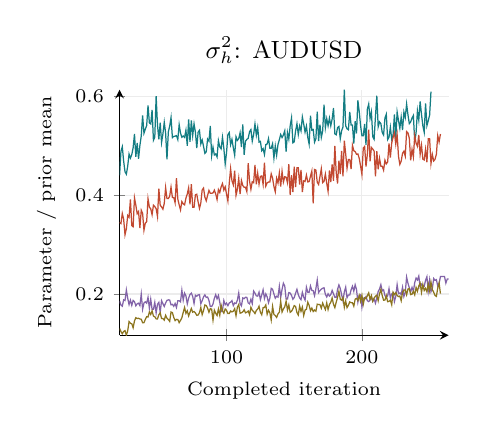
\begin{tikzpicture}
\begin{axis}[width=.475\linewidth,height=4.7cm,title={$\sigma^2_h$: AUDUSD},
 title style={font=\small},xlabel={Completed iteration},ylabel={Parameter / prior mean},
 axis lines=left,grid=major,grid style={gray!15},
 tick label style={font=\scriptsize},label style={font=\scriptsize},scaled ticks=false]
\addplot[chainone,line width=.45pt,no marks] coordinates {(21,0.440004) (22,0.488331) (23,0.497883) (24,0.468609) (25,0.447381) (26,0.442396) (27,0.458878) (28,0.483259) (29,0.474974) (30,0.481971) (31,0.495865) (32,0.523788) (33,0.477478) (34,0.505462) (35,0.473605) (36,0.500386) (37,0.519641) (38,0.561172) (39,0.525216) (40,0.533485) (41,0.540594) (42,0.581474) (43,0.546073) (44,0.544015) (45,0.572305) (46,0.510976) (47,0.517199) (48,0.600211) (49,0.541223) (50,0.512818) (51,0.546481) (52,0.506462) (53,0.523682) (54,0.547403) (55,0.525371) (56,0.472379) (57,0.52779) (58,0.539645) (59,0.55693) (60,0.516323) (61,0.51878) (62,0.519287) (63,0.520385) (64,0.512321) (65,0.542551) (66,0.525615) (67,0.517064) (68,0.519734) (69,0.516757) (70,0.531252) (71,0.499883) (72,0.553382) (73,0.507755) (74,0.55125) (75,0.520439) (76,0.544115) (77,0.527231) (78,0.495087) (79,0.527188) (80,0.531097) (81,0.503626) (82,0.511664) (83,0.498734) (84,0.484452) (85,0.487584) (86,0.513432) (87,0.509154) (88,0.539782) (89,0.479862) (90,0.497044) (91,0.481155) (92,0.483391) (93,0.477203) (94,0.510201) (95,0.497403) (96,0.4936) (97,0.516855) (98,0.494842) (99,0.463093) (100,0.486097) (101,0.52251) (102,0.526492) (103,0.502059) (104,0.512746) (105,0.495613) (106,0.480715) (107,0.518099) (108,0.510731) (109,0.514297) (110,0.526169) (111,0.49737) (112,0.542993) (113,0.481357) (114,0.509179) (115,0.512581) (116,0.515063) (117,0.528249) (118,0.532597) (119,0.509099) (120,0.522647) (121,0.543928) (122,0.521233) (123,0.536933) (124,0.507389) (125,0.508691) (126,0.489918) (127,0.494058) (128,0.482168) (129,0.502293) (130,0.503386) (131,0.51447) (132,0.494971) (133,0.494933) (134,0.503945) (135,0.474792) (136,0.499502) (137,0.480529) (138,0.502453) (139,0.512176) (140,0.522635) (141,0.516526) (142,0.521724) (143,0.52997) (144,0.487853) (145,0.526647) (146,0.513311) (147,0.540072) (148,0.556131) (149,0.505702) (150,0.507828) (151,0.529817) (152,0.544298) (153,0.522541) (154,0.539709) (155,0.53) (156,0.558131) (157,0.543779) (158,0.527305) (159,0.539649) (160,0.51695) (161,0.503265) (162,0.560637) (163,0.531297) (164,0.532637) (165,0.507249) (166,0.514056) (167,0.568815) (168,0.509531) (169,0.542654) (170,0.51654) (171,0.52978) (172,0.582833) (173,0.536279) (174,0.554753) (175,0.54021) (176,0.555844) (177,0.540211) (178,0.553992) (179,0.576114) (180,0.523915) (181,0.522063) (182,0.536581) (183,0.538881) (184,0.514017) (185,0.530065) (186,0.537906) (187,0.613187) (188,0.540046) (189,0.534196) (190,0.532239) (191,0.568493) (192,0.541773) (193,0.541615) (194,0.504302) (195,0.549559) (196,0.524747) (197,0.591704) (198,0.569187) (199,0.540589) (200,0.520045) (201,0.520045) (202,0.543832) (203,0.501794) (204,0.57335) (205,0.584242) (206,0.555207) (207,0.568241) (208,0.517901) (209,0.512833) (210,0.559455) (211,0.600916) (212,0.538139) (213,0.547962) (214,0.54456) (215,0.526716) (216,0.521535) (217,0.556067) (218,0.563459) (219,0.512362) (220,0.517134) (221,0.537418) (222,0.513069) (223,0.521496) (224,0.563259) (225,0.515056) (226,0.568148) (227,0.551058) (228,0.535185) (229,0.557659) (230,0.53166) (231,0.568125) (232,0.556829) (233,0.584236) (234,0.562272) (235,0.54463) (236,0.548078) (237,0.555861) (238,0.561175) (239,0.507407) (240,0.526282) (241,0.570607) (242,0.551718) (243,0.589382) (244,0.563427) (245,0.540297) (246,0.527067) (247,0.585679) (248,0.540467) (249,0.550589) (250,0.561928) (251,0.609162)};
\addplot[chaintwo,line width=.45pt,no marks] coordinates {(21,0.345037) (22,0.342518) (23,0.362983) (24,0.351366) (25,0.319833) (26,0.332225) (27,0.358848) (28,0.355354) (29,0.391482) (30,0.338581) (31,0.33606) (32,0.394684) (33,0.379695) (34,0.362517) (35,0.3669) (36,0.333638) (37,0.369577) (38,0.36314) (39,0.329018) (40,0.343477) (41,0.346313) (42,0.392775) (43,0.375783) (44,0.372382) (45,0.360352) (46,0.379747) (47,0.376804) (48,0.372629) (49,0.356634) (50,0.413119) (51,0.379537) (52,0.376388) (53,0.371654) (54,0.383433) (55,0.415329) (56,0.39303) (57,0.393) (58,0.397951) (59,0.416253) (60,0.395365) (61,0.395368) (62,0.38471) (63,0.434354) (64,0.392043) (65,0.380561) (66,0.370147) (67,0.38698) (68,0.382323) (69,0.380394) (70,0.393818) (71,0.402336) (72,0.41495) (73,0.381298) (74,0.422367) (75,0.375458) (76,0.375458) (77,0.400801) (78,0.401861) (79,0.386481) (80,0.373149) (81,0.384396) (82,0.4104) (83,0.414318) (84,0.396138) (85,0.388555) (86,0.399387) (87,0.409541) (88,0.403746) (89,0.403746) (90,0.40453) (91,0.410048) (92,0.402373) (93,0.391258) (94,0.41126) (95,0.405287) (96,0.41658) (97,0.423367) (98,0.410205) (99,0.416852) (100,0.402023) (101,0.388262) (102,0.424114) (103,0.453321) (104,0.429044) (105,0.420877) (106,0.449539) (107,0.399597) (108,0.41202) (109,0.433974) (110,0.4022) (111,0.429645) (112,0.419466) (113,0.41582) (114,0.4161) (115,0.407113) (116,0.464776) (117,0.428127) (118,0.411663) (119,0.427128) (120,0.425207) (121,0.461044) (122,0.42199) (123,0.44416) (124,0.422182) (125,0.437863) (126,0.438833) (127,0.421878) (128,0.465639) (129,0.418343) (130,0.42487) (131,0.426491) (132,0.426491) (133,0.443044) (134,0.434294) (135,0.417481) (136,0.406732) (137,0.434058) (138,0.424467) (139,0.444828) (140,0.417177) (141,0.448063) (142,0.426434) (143,0.437199) (144,0.436339) (145,0.425201) (146,0.462526) (147,0.400824) (148,0.440149) (149,0.406153) (150,0.457557) (151,0.416431) (152,0.455382) (153,0.455382) (154,0.421544) (155,0.451103) (156,0.406257) (157,0.428711) (158,0.427711) (159,0.440435) (160,0.426701) (161,0.427511) (162,0.438297) (163,0.448712) (164,0.383485) (165,0.4519) (166,0.450569) (167,0.425922) (168,0.421523) (169,0.43764) (170,0.453284) (171,0.425291) (172,0.427821) (173,0.442652) (174,0.424092) (175,0.407707) (176,0.450137) (177,0.426324) (178,0.462353) (179,0.429131) (180,0.499666) (181,0.445646) (182,0.423638) (183,0.469884) (184,0.442693) (185,0.489312) (186,0.437841) (187,0.510145) (188,0.483258) (189,0.454379) (190,0.472328) (191,0.472328) (192,0.452699) (193,0.500959) (194,0.489706) (195,0.487916) (196,0.482711) (197,0.483308) (198,0.474566) (199,0.45874) (200,0.441739) (201,0.495335) (202,0.498388) (203,0.457647) (204,0.482364) (205,0.53223) (206,0.468506) (207,0.496302) (208,0.493155) (209,0.489131) (210,0.438215) (211,0.488981) (212,0.452315) (213,0.47452) (214,0.458581) (215,0.458236) (216,0.450449) (217,0.470627) (218,0.463151) (219,0.467042) (220,0.504766) (221,0.476039) (222,0.505752) (223,0.516835) (224,0.525944) (225,0.503262) (226,0.522449) (227,0.478726) (228,0.462155) (229,0.468774) (230,0.484546) (231,0.488834) (232,0.4788) (233,0.528598) (234,0.525805) (235,0.515112) (236,0.470224) (237,0.492529) (238,0.477362) (239,0.520397) (240,0.504939) (241,0.49868) (242,0.52171) (243,0.482228) (244,0.501125) (245,0.472821) (246,0.471203) (247,0.492737) (248,0.466602) (249,0.514071) (250,0.513936) (251,0.463835) (252,0.482406) (253,0.469115) (254,0.47253) (255,0.482746) (256,0.520295) (257,0.507417) (258,0.523612)};
\addplot[chainthree,line width=.45pt,no marks] coordinates {(21,0.185989) (22,0.177696) (23,0.175485) (24,0.18824) (25,0.187003) (26,0.20824) (27,0.191409) (28,0.178697) (29,0.187682) (30,0.177228) (31,0.187036) (32,0.184601) (33,0.176238) (34,0.180432) (35,0.181498) (36,0.176491) (37,0.200018) (38,0.169194) (39,0.181804) (40,0.184283) (41,0.181517) (42,0.193475) (43,0.171293) (44,0.189498) (45,0.16905) (46,0.16905) (47,0.183164) (48,0.16189) (49,0.179174) (50,0.183214) (51,0.163216) (52,0.186553) (53,0.180494) (54,0.174914) (55,0.182079) (56,0.187149) (57,0.188305) (58,0.187843) (59,0.178157) (60,0.179172) (61,0.175226) (62,0.18092) (63,0.172956) (64,0.186322) (65,0.186507) (66,0.184288) (67,0.207824) (68,0.18765) (69,0.201956) (70,0.196376) (71,0.180148) (72,0.191536) (73,0.199174) (74,0.202005) (75,0.195223) (76,0.181036) (77,0.197599) (78,0.195595) (79,0.198079) (80,0.198852) (81,0.180247) (82,0.186546) (83,0.194177) (84,0.198302) (85,0.193243) (86,0.193935) (87,0.187201) (88,0.174684) (89,0.17471) (90,0.179979) (91,0.191316) (92,0.198764) (93,0.190234) (94,0.197118) (95,0.183402) (96,0.164467) (97,0.166522) (98,0.186986) (99,0.178362) (100,0.181692) (101,0.176522) (102,0.181942) (103,0.183634) (104,0.18663) (105,0.176683) (106,0.181994) (107,0.180855) (108,0.187491) (109,0.202237) (110,0.180539) (111,0.176146) (112,0.192137) (113,0.19073) (114,0.19363) (115,0.19322) (116,0.182011) (117,0.180132) (118,0.189596) (119,0.180626) (120,0.206059) (121,0.201877) (122,0.196386) (123,0.195761) (124,0.20377) (125,0.188576) (126,0.198173) (127,0.208474) (128,0.190907) (129,0.20028) (130,0.194219) (131,0.18246) (132,0.191894) (133,0.211568) (134,0.209749) (135,0.200173) (136,0.191398) (137,0.195538) (138,0.193867) (139,0.215686) (140,0.193036) (141,0.209242) (142,0.221832) (143,0.215984) (144,0.189842) (145,0.189842) (146,0.20295) (147,0.202051) (148,0.197242) (149,0.189471) (150,0.192925) (151,0.201717) (152,0.209477) (153,0.198714) (154,0.19201) (155,0.188529) (156,0.203422) (157,0.193599) (158,0.187873) (159,0.213907) (160,0.203812) (161,0.203466) (162,0.216329) (163,0.207304) (164,0.206755) (165,0.196671) (166,0.211201) (167,0.228463) (168,0.203051) (169,0.206957) (170,0.209995) (171,0.211686) (172,0.21264) (173,0.199304) (174,0.194058) (175,0.200532) (176,0.195929) (177,0.199051) (178,0.207496) (179,0.200359) (180,0.19363) (181,0.19363) (182,0.20972) (183,0.218442) (184,0.211339) (185,0.19886) (186,0.18643) (187,0.204391) (188,0.213967) (189,0.19248) (190,0.198004) (191,0.197957) (192,0.208447) (193,0.215717) (194,0.205659) (195,0.218683) (196,0.209323) (197,0.183828) (198,0.197168) (199,0.198433) (200,0.173534) (201,0.191634) (202,0.190049) (203,0.194803) (204,0.186682) (205,0.184748) (206,0.187932) (207,0.19292) (208,0.18535) (209,0.189834) (210,0.181503) (211,0.192925) (212,0.205172) (213,0.210254) (214,0.218836) (215,0.206427) (216,0.208618) (217,0.196627) (218,0.193815) (219,0.19618) (220,0.210815) (221,0.19235) (222,0.200182) (223,0.202443) (224,0.184788) (225,0.195261) (226,0.218915) (227,0.20085) (228,0.202245) (229,0.1993) (230,0.213647) (231,0.194971) (232,0.203315) (233,0.234269) (234,0.221762) (235,0.212735) (236,0.204297) (237,0.213376) (238,0.205484) (239,0.223171) (240,0.232346) (241,0.228451) (242,0.236346) (243,0.214254) (244,0.219953) (245,0.216511) (246,0.215444) (247,0.227716) (248,0.235091) (249,0.206345) (250,0.227967) (251,0.204724) (252,0.211175) (253,0.231462) (254,0.227663) (255,0.229074) (256,0.216371) (257,0.221613) (258,0.235352) (259,0.235287) (260,0.235287) (261,0.235287) (262,0.222016) (263,0.230299) (264,0.230398)};
\addplot[chainfour,line width=.45pt,no marks] coordinates {(21,0.130425) (22,0.124104) (23,0.119644) (24,0.124431) (25,0.125984) (26,0.116671) (27,0.125641) (28,0.144363) (29,0.140905) (30,0.139899) (31,0.13184) (32,0.14565) (33,0.152147) (34,0.150411) (35,0.151052) (36,0.149708) (37,0.148972) (38,0.142042) (39,0.142178) (40,0.148671) (41,0.154335) (42,0.153528) (43,0.163712) (44,0.158757) (45,0.166017) (46,0.155523) (47,0.154032) (48,0.149835) (49,0.149638) (50,0.158098) (51,0.162118) (52,0.150714) (53,0.150525) (54,0.147211) (55,0.157051) (56,0.150989) (57,0.148556) (58,0.14473) (59,0.163667) (60,0.162473) (61,0.152912) (62,0.146279) (63,0.148788) (64,0.148674) (65,0.142193) (66,0.146725) (67,0.151995) (68,0.162868) (69,0.172913) (70,0.160978) (71,0.166028) (72,0.15572) (73,0.163115) (74,0.170845) (75,0.163301) (76,0.164778) (77,0.162014) (78,0.156935) (79,0.157581) (80,0.162329) (81,0.172788) (82,0.158364) (83,0.166574) (84,0.177814) (85,0.176739) (86,0.171666) (87,0.163256) (88,0.17052) (89,0.169502) (90,0.147216) (91,0.167353) (92,0.161111) (93,0.156635) (94,0.169843) (95,0.15709) (96,0.177197) (97,0.166021) (98,0.161397) (99,0.169902) (100,0.167008) (101,0.160525) (102,0.160518) (103,0.165865) (104,0.16382) (105,0.165317) (106,0.170355) (107,0.156065) (108,0.173301) (109,0.178686) (110,0.161296) (111,0.162234) (112,0.163924) (113,0.168231) (114,0.161918) (115,0.16321) (116,0.165703) (117,0.158507) (118,0.173207) (119,0.167165) (120,0.164612) (121,0.160563) (122,0.166844) (123,0.169534) (124,0.175296) (125,0.163186) (126,0.158097) (127,0.172552) (128,0.172628) (129,0.177846) (130,0.15915) (131,0.167331) (132,0.162004) (133,0.147485) (134,0.174923) (135,0.158773) (136,0.156554) (137,0.152709) (138,0.159932) (139,0.163415) (140,0.185451) (141,0.163571) (142,0.169876) (143,0.17417) (144,0.185529) (145,0.167668) (146,0.178005) (147,0.163034) (148,0.165116) (149,0.170317) (150,0.176649) (151,0.174894) (152,0.162616) (153,0.157585) (154,0.175469) (155,0.165086) (156,0.173621) (157,0.156537) (158,0.167658) (159,0.169117) (160,0.183617) (161,0.177122) (162,0.16638) (163,0.171724) (164,0.164633) (165,0.167674) (166,0.165267) (167,0.179542) (168,0.178907) (169,0.178574) (170,0.171295) (171,0.18174) (172,0.174975) (173,0.168643) (174,0.182161) (175,0.168621) (176,0.178704) (177,0.183522) (178,0.191988) (179,0.179255) (180,0.172634) (181,0.183476) (182,0.193131) (183,0.205562) (184,0.189427) (185,0.187676) (186,0.192933) (187,0.173137) (188,0.186167) (189,0.172619) (190,0.177225) (191,0.184107) (192,0.182588) (193,0.182254) (194,0.175396) (195,0.189693) (196,0.191304) (197,0.186989) (198,0.196918) (199,0.185191) (200,0.197556) (201,0.179474) (202,0.192413) (203,0.190566) (204,0.196687) (205,0.202311) (206,0.189191) (207,0.196799) (208,0.185496) (209,0.192175) (210,0.195446) (211,0.197911) (212,0.186538) (213,0.200325) (214,0.209289) (215,0.196657) (216,0.187604) (217,0.187792) (218,0.196756) (219,0.184508) (220,0.185242) (221,0.187609) (222,0.178412) (223,0.203697) (224,0.198938) (225,0.202956) (226,0.197207) (227,0.194924) (228,0.19598) (229,0.186442) (230,0.20343) (231,0.20806) (232,0.208327) (233,0.198479) (234,0.210192) (235,0.210929) (236,0.198885) (237,0.19968) (238,0.205589) (239,0.198498) (240,0.213318) (241,0.205558) (242,0.216195) (243,0.221742) (244,0.203317) (245,0.21925) (246,0.207084) (247,0.211651) (248,0.204682) (249,0.220305) (250,0.206705) (251,0.224347) (252,0.209056) (253,0.203656) (254,0.197119) (255,0.19531) (256,0.212105) (257,0.222376) (258,0.200772)};
\end{axis}\end{tikzpicture}\hfill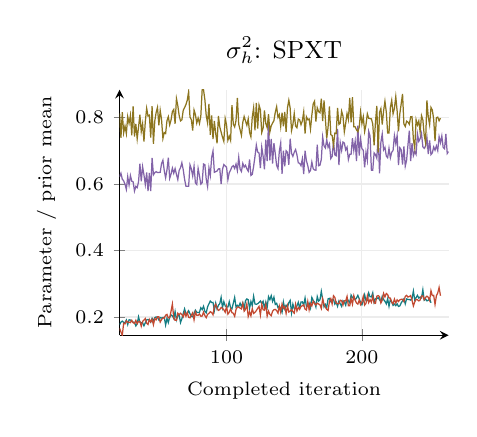
\begin{tikzpicture}
\begin{axis}[width=.475\linewidth,height=4.7cm,title={$\sigma^2_h$: SPXT},
 title style={font=\small},xlabel={Completed iteration},ylabel={Parameter / prior mean},
 axis lines=left,grid=major,grid style={gray!15},
 tick label style={font=\scriptsize},label style={font=\scriptsize},scaled ticks=false]
\addplot[chainone,line width=.45pt,no marks] coordinates {(21,0.176121) (22,0.184716) (23,0.187732) (24,0.183668) (25,0.182337) (26,0.190788) (27,0.177114) (28,0.191419) (29,0.191252) (30,0.187525) (31,0.184403) (32,0.183831) (33,0.173162) (34,0.179526) (35,0.200541) (36,0.184448) (37,0.182407) (38,0.182501) (39,0.173351) (40,0.182654) (41,0.191198) (42,0.192616) (43,0.189802) (44,0.184282) (45,0.196228) (46,0.188954) (47,0.197981) (48,0.200117) (49,0.199123) (50,0.19135) (51,0.198356) (52,0.196644) (53,0.198656) (54,0.199002) (55,0.175706) (56,0.196514) (57,0.183118) (58,0.199507) (59,0.206352) (60,0.203242) (61,0.195619) (62,0.216705) (63,0.191424) (64,0.204011) (65,0.205966) (66,0.183139) (67,0.19473) (68,0.21058) (69,0.224663) (70,0.21044) (71,0.210502) (72,0.218632) (73,0.20979) (74,0.201773) (75,0.200563) (76,0.21043) (77,0.220687) (78,0.21423) (79,0.213588) (80,0.2142) (81,0.227799) (82,0.222263) (83,0.232257) (84,0.217133) (85,0.212353) (86,0.230808) (87,0.239659) (88,0.248061) (89,0.243444) (90,0.243875) (91,0.219355) (92,0.241721) (93,0.224073) (94,0.235325) (95,0.240381) (96,0.259016) (97,0.228193) (98,0.246295) (99,0.233579) (100,0.229805) (101,0.229819) (102,0.246037) (103,0.227715) (104,0.224517) (105,0.24168) (106,0.258992) (107,0.229778) (108,0.235086) (109,0.231422) (110,0.241743) (111,0.231333) (112,0.242455) (113,0.225121) (114,0.249214) (115,0.254342) (116,0.251994) (117,0.225981) (118,0.246813) (119,0.234156) (120,0.262434) (121,0.239233) (122,0.238143) (123,0.239984) (124,0.243457) (125,0.248076) (126,0.240268) (127,0.247425) (128,0.226406) (129,0.245009) (130,0.229038) (131,0.26129) (132,0.251999) (133,0.264162) (134,0.246928) (135,0.259637) (136,0.237751) (137,0.241121) (138,0.228414) (139,0.232626) (140,0.225088) (141,0.214125) (142,0.245143) (143,0.225024) (144,0.235431) (145,0.230026) (146,0.243061) (147,0.249944) (148,0.212566) (149,0.238606) (150,0.224998) (151,0.226226) (152,0.2336) (153,0.244228) (154,0.227195) (155,0.245019) (156,0.245478) (157,0.235448) (158,0.257287) (159,0.231756) (160,0.231328) (161,0.241338) (162,0.227258) (163,0.258789) (164,0.250134) (165,0.24423) (166,0.230322) (167,0.261433) (168,0.247822) (169,0.251841) (170,0.27718) (171,0.253358) (172,0.230532) (173,0.237904) (174,0.228754) (175,0.254542) (176,0.255967) (177,0.246505) (178,0.252653) (179,0.252653) (180,0.23875) (181,0.244294) (182,0.231983) (183,0.247789) (184,0.239915) (185,0.231802) (186,0.249153) (187,0.244891) (188,0.235483) (189,0.25538) (190,0.249346) (191,0.242525) (192,0.266006) (193,0.258262) (194,0.260886) (195,0.252037) (196,0.256946) (197,0.265006) (198,0.254573) (199,0.24399) (200,0.236751) (201,0.247855) (202,0.266724) (203,0.249834) (204,0.249562) (205,0.272175) (206,0.260676) (207,0.260488) (208,0.272871) (209,0.243996) (210,0.25516) (211,0.25516) (212,0.258164) (213,0.251906) (214,0.245779) (215,0.26228) (216,0.252288) (217,0.247344) (218,0.23932) (219,0.25483) (220,0.232062) (221,0.253006) (222,0.245139) (223,0.234968) (224,0.238844) (225,0.234128) (226,0.239913) (227,0.23171) (228,0.233232) (229,0.242345) (230,0.248395) (231,0.25458) (232,0.239471) (233,0.25448) (234,0.252775) (235,0.252686) (236,0.250757) (237,0.254275) (238,0.278072) (239,0.251701) (240,0.257931) (241,0.265197) (242,0.256749) (243,0.260183) (244,0.257489) (245,0.282126) (246,0.250576) (247,0.254476) (248,0.248522) (249,0.250439) (250,0.254719) (251,0.242787)};
\addplot[chaintwo,line width=.45pt,no marks] coordinates {(21,0.166018) (22,0.155034) (23,0.145091) (24,0.180903) (25,0.179433) (26,0.188283) (27,0.184398) (28,0.184271) (29,0.183181) (30,0.189975) (31,0.182996) (32,0.180291) (33,0.189828) (34,0.179597) (35,0.186754) (36,0.186754) (37,0.172142) (38,0.186582) (39,0.190476) (40,0.195495) (41,0.181732) (42,0.1776) (43,0.192811) (44,0.185314) (45,0.193211) (46,0.176538) (47,0.195643) (48,0.191497) (49,0.200561) (50,0.200561) (51,0.184836) (52,0.192305) (53,0.197158) (54,0.196462) (55,0.20555) (56,0.207897) (57,0.197324) (58,0.197906) (59,0.217275) (60,0.239063) (61,0.19821) (62,0.190047) (63,0.190047) (64,0.211441) (65,0.206914) (66,0.211549) (67,0.207462) (68,0.200227) (69,0.213743) (70,0.202102) (71,0.213561) (72,0.198857) (73,0.197593) (74,0.205546) (75,0.212902) (76,0.191382) (77,0.215489) (78,0.205207) (79,0.205073) (80,0.209195) (81,0.202315) (82,0.202942) (83,0.214798) (84,0.204155) (85,0.198027) (86,0.207965) (87,0.210851) (88,0.215962) (89,0.213514) (90,0.206637) (91,0.231284) (92,0.238498) (93,0.226547) (94,0.219895) (95,0.222194) (96,0.22864) (97,0.226254) (98,0.221681) (99,0.214399) (100,0.232469) (101,0.208663) (102,0.214004) (103,0.224591) (104,0.213028) (105,0.211269) (106,0.202162) (107,0.222662) (108,0.230087) (109,0.22962) (110,0.226798) (111,0.224226) (112,0.240906) (113,0.217393) (114,0.222802) (115,0.239796) (116,0.201711) (117,0.215397) (118,0.203139) (119,0.22505) (120,0.210833) (121,0.213864) (122,0.219191) (123,0.225995) (124,0.231871) (125,0.205947) (126,0.23864) (127,0.221646) (128,0.220846) (129,0.238001) (130,0.202854) (131,0.217765) (132,0.207646) (133,0.203814) (134,0.217557) (135,0.221971) (136,0.222882) (137,0.219411) (138,0.211681) (139,0.232855) (140,0.21453) (141,0.239206) (142,0.226212) (143,0.231678) (144,0.210818) (145,0.233849) (146,0.214983) (147,0.217661) (148,0.222579) (149,0.216072) (150,0.211405) (151,0.238084) (152,0.218077) (153,0.228597) (154,0.223058) (155,0.231689) (156,0.233864) (157,0.237312) (158,0.223834) (159,0.221054) (160,0.246356) (161,0.22138) (162,0.240632) (163,0.233364) (164,0.247644) (165,0.240306) (166,0.236226) (167,0.241558) (168,0.239053) (169,0.23674) (170,0.225568) (171,0.254513) (172,0.238717) (173,0.229691) (174,0.222901) (175,0.219725) (176,0.246694) (177,0.254986) (178,0.238978) (179,0.263922) (180,0.258868) (181,0.241483) (182,0.240266) (183,0.239977) (184,0.250471) (185,0.249275) (186,0.235897) (187,0.24899) (188,0.248185) (189,0.261949) (190,0.233616) (191,0.23404) (192,0.255459) (193,0.238404) (194,0.264266) (195,0.250801) (196,0.242169) (197,0.238703) (198,0.250511) (199,0.237308) (200,0.246071) (201,0.26215) (202,0.235853) (203,0.240985) (204,0.2635) (205,0.243314) (206,0.252082) (207,0.244301) (208,0.2624) (209,0.242218) (210,0.241117) (211,0.262658) (212,0.26439) (213,0.261257) (214,0.242112) (215,0.25066) (216,0.27097) (217,0.260364) (218,0.270696) (219,0.267175) (220,0.256904) (221,0.256772) (222,0.244302) (223,0.239449) (224,0.253689) (225,0.242104) (226,0.251674) (227,0.246518) (228,0.251714) (229,0.253125) (230,0.253227) (231,0.246688) (232,0.261909) (233,0.265142) (234,0.259914) (235,0.261616) (236,0.264492) (237,0.250161) (238,0.233219) (239,0.245142) (240,0.253056) (241,0.25214) (242,0.248422) (243,0.25113) (244,0.263139) (245,0.263543) (246,0.252121) (247,0.258989) (248,0.262541) (249,0.259311) (250,0.249954) (251,0.279263) (252,0.264388) (253,0.26517) (254,0.237624) (255,0.263882) (256,0.272401) (257,0.288949) (258,0.263969)};
\addplot[chainthree,line width=.45pt,no marks] coordinates {(21,0.621642) (22,0.632225) (23,0.614331) (24,0.609637) (25,0.599378) (26,0.583761) (27,0.622429) (28,0.597205) (29,0.625433) (30,0.608494) (31,0.60649) (32,0.578844) (33,0.592884) (34,0.589053) (35,0.606805) (36,0.660907) (37,0.607897) (38,0.651899) (39,0.627277) (40,0.598419) (41,0.634651) (42,0.578406) (43,0.633461) (44,0.57871) (45,0.678491) (46,0.627631) (47,0.633997) (48,0.637256) (49,0.634546) (50,0.63475) (51,0.635218) (52,0.661605) (53,0.671592) (54,0.639977) (55,0.618663) (56,0.642515) (57,0.678973) (58,0.617112) (59,0.629738) (60,0.647907) (61,0.632421) (62,0.646269) (63,0.629167) (64,0.613532) (65,0.641024) (66,0.648704) (67,0.663916) (68,0.643344) (69,0.614625) (70,0.593404) (71,0.593404) (72,0.593404) (73,0.657485) (74,0.645281) (75,0.624027) (76,0.653344) (77,0.603217) (78,0.598654) (79,0.646939) (80,0.624711) (81,0.599664) (82,0.60403) (83,0.660094) (84,0.65813) (85,0.614157) (86,0.592242) (87,0.64867) (88,0.625357) (89,0.679744) (90,0.699509) (91,0.6352) (92,0.637421) (93,0.639043) (94,0.645555) (95,0.645649) (96,0.600194) (97,0.643795) (98,0.658378) (99,0.654064) (100,0.650902) (101,0.613075) (102,0.634262) (103,0.642081) (104,0.651832) (105,0.655244) (106,0.646637) (107,0.660018) (108,0.640525) (109,0.680396) (110,0.645008) (111,0.637726) (112,0.66224) (113,0.650819) (114,0.65643) (115,0.645905) (116,0.638543) (117,0.673689) (118,0.625744) (119,0.628974) (120,0.653183) (121,0.682767) (122,0.717129) (123,0.696295) (124,0.693421) (125,0.647629) (126,0.710608) (127,0.684221) (128,0.644049) (129,0.733409) (130,0.668973) (131,0.788346) (132,0.671152) (133,0.735856) (134,0.661115) (135,0.722966) (136,0.691184) (137,0.655753) (138,0.646353) (139,0.699345) (140,0.723479) (141,0.630318) (142,0.700211) (143,0.653407) (144,0.700086) (145,0.695948) (146,0.657938) (147,0.736039) (148,0.692414) (149,0.683204) (150,0.695446) (151,0.703678) (152,0.687978) (153,0.663642) (154,0.662324) (155,0.655126) (156,0.675799) (157,0.630201) (158,0.700474) (159,0.669909) (160,0.65525) (161,0.635082) (162,0.640629) (163,0.666009) (164,0.645899) (165,0.642033) (166,0.641588) (167,0.718623) (168,0.654976) (169,0.656659) (170,0.673957) (171,0.741468) (172,0.714659) (173,0.708375) (174,0.733246) (175,0.710357) (176,0.720599) (177,0.676569) (178,0.683372) (179,0.727856) (180,0.687471) (181,0.685129) (182,0.76602) (183,0.657025) (184,0.723684) (185,0.700733) (186,0.726298) (187,0.72346) (188,0.702699) (189,0.710816) (190,0.673457) (191,0.689424) (192,0.689556) (193,0.737638) (194,0.701076) (195,0.728503) (196,0.668894) (197,0.775335) (198,0.685798) (199,0.735272) (200,0.70622) (201,0.701678) (202,0.650116) (203,0.696069) (204,0.671674) (205,0.758114) (206,0.744416) (207,0.641763) (208,0.641763) (209,0.693641) (210,0.688056) (211,0.677584) (212,0.745272) (213,0.632059) (214,0.725636) (215,0.750264) (216,0.70261) (217,0.710427) (218,0.684282) (219,0.679021) (220,0.707545) (221,0.678909) (222,0.695514) (223,0.700874) (224,0.745682) (225,0.721642) (226,0.745522) (227,0.656884) (228,0.709287) (229,0.702853) (230,0.658839) (231,0.71311) (232,0.653548) (233,0.671427) (234,0.7176) (235,0.760649) (236,0.668969) (237,0.723068) (238,0.685243) (239,0.697248) (240,0.689185) (241,0.751219) (242,0.728371) (243,0.736774) (244,0.752508) (245,0.712057) (246,0.70728) (247,0.714215) (248,0.740359) (249,0.690115) (250,0.731051) (251,0.688594) (252,0.693423) (253,0.711434) (254,0.701774) (255,0.714924) (256,0.700774) (257,0.742375) (258,0.724478) (259,0.744609) (260,0.710071) (261,0.706153) (262,0.750991) (263,0.691797) (264,0.697507)};
\addplot[chainfour,line width=.45pt,no marks] coordinates {(21,0.812411) (22,0.738814) (23,0.815952) (24,0.753774) (25,0.774585) (26,0.751606) (27,0.802779) (28,0.782683) (29,0.806415) (30,0.746766) (31,0.833606) (32,0.743027) (33,0.780581) (34,0.735705) (35,0.77145) (36,0.808258) (37,0.757882) (38,0.781244) (39,0.727685) (40,0.787739) (41,0.827589) (42,0.804483) (43,0.807011) (44,0.739521) (45,0.833907) (46,0.720938) (47,0.789823) (48,0.815133) (49,0.830672) (50,0.776286) (51,0.821437) (52,0.793352) (53,0.737) (54,0.754485) (55,0.751767) (56,0.790699) (57,0.802436) (58,0.777906) (59,0.792342) (60,0.817799) (61,0.824253) (62,0.781417) (63,0.856963) (64,0.835979) (65,0.806239) (66,0.789809) (67,0.79293) (68,0.821311) (69,0.829664) (70,0.839049) (71,0.852088) (72,0.878301) (73,0.801269) (74,0.793672) (75,0.760716) (76,0.822408) (77,0.808841) (78,0.78332) (79,0.79859) (80,0.782048) (81,0.803964) (82,0.883647) (83,0.883647) (84,0.853399) (85,0.805435) (86,0.783316) (87,0.840673) (88,0.748075) (89,0.806427) (90,0.734931) (91,0.78942) (92,0.751581) (93,0.72222) (94,0.804503) (95,0.771615) (96,0.756384) (97,0.740774) (98,0.728487) (99,0.797119) (100,0.777821) (101,0.731493) (102,0.743749) (103,0.73094) (104,0.837107) (105,0.780526) (106,0.77188) (107,0.790839) (108,0.858695) (109,0.779519) (110,0.7633) (111,0.746143) (112,0.78556) (113,0.803149) (114,0.789667) (115,0.776745) (116,0.795674) (117,0.75557) (118,0.741825) (119,0.801502) (120,0.829457) (121,0.761399) (122,0.844052) (123,0.766596) (124,0.837544) (125,0.823369) (126,0.754766) (127,0.767932) (128,0.821151) (129,0.781821) (130,0.769342) (131,0.810153) (132,0.75663) (133,0.775054) (134,0.782989) (135,0.790868) (136,0.815811) (137,0.832603) (138,0.800353) (139,0.808891) (140,0.77358) (141,0.814454) (142,0.773441) (143,0.816584) (144,0.756703) (145,0.828923) (146,0.852043) (147,0.827998) (148,0.760578) (149,0.77853) (150,0.811985) (151,0.774184) (152,0.769202) (153,0.795351) (154,0.793015) (155,0.778342) (156,0.790321) (157,0.817029) (158,0.751978) (159,0.802204) (160,0.793521) (161,0.795726) (162,0.765198) (163,0.806939) (164,0.840791) (165,0.848902) (166,0.787934) (167,0.829513) (168,0.817989) (169,0.814246) (170,0.85679) (171,0.789124) (172,0.851174) (173,0.796247) (174,0.73717) (175,0.771357) (176,0.833391) (177,0.748714) (178,0.745649) (179,0.717001) (180,0.753284) (181,0.752124) (182,0.829063) (183,0.779169) (184,0.783161) (185,0.819147) (186,0.804337) (187,0.756882) (188,0.782242) (189,0.8121) (190,0.794213) (191,0.859157) (192,0.785321) (193,0.861315) (194,0.772187) (195,0.77192) (196,0.762876) (197,0.757205) (198,0.771127) (199,0.816521) (200,0.781779) (201,0.801833) (202,0.757869) (203,0.778374) (204,0.811237) (205,0.797767) (206,0.796975) (207,0.795968) (208,0.780575) (209,0.716157) (210,0.786628) (211,0.835117) (212,0.695036) (213,0.815501) (214,0.826932) (215,0.779121) (216,0.820061) (217,0.848923) (218,0.816691) (219,0.753613) (220,0.753613) (221,0.829678) (222,0.851646) (223,0.811313) (224,0.827604) (225,0.863075) (226,0.81968) (227,0.758233) (228,0.811764) (229,0.841114) (230,0.871105) (231,0.780668) (232,0.772938) (233,0.78902) (234,0.786259) (235,0.779586) (236,0.80213) (237,0.80265) (238,0.734371) (239,0.707999) (240,0.793323) (241,0.777608) (242,0.789838) (243,0.755812) (244,0.805627) (245,0.792982) (246,0.747239) (247,0.724144) (248,0.851766) (249,0.801733) (250,0.778206) (251,0.830263) (252,0.822557) (253,0.794637) (254,0.729068) (255,0.799546) (256,0.801117) (257,0.790274) (258,0.798083)};
\end{axis}\end{tikzpicture}
\par\smallskip
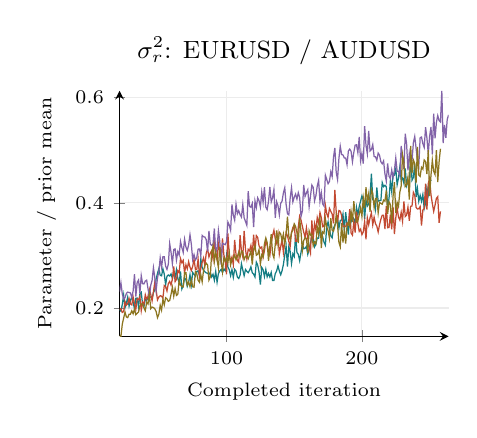
\begin{tikzpicture}
\begin{axis}[width=.475\linewidth,height=4.7cm,title={$\sigma^2_r$: EURUSD / AUDUSD},
 title style={font=\small},xlabel={Completed iteration},ylabel={Parameter / prior mean},
 axis lines=left,grid=major,grid style={gray!15},
 tick label style={font=\scriptsize},label style={font=\scriptsize},scaled ticks=false]
\addplot[chainone,line width=.45pt,no marks] coordinates {(21,0.196539) (22,0.193847) (23,0.20697) (24,0.224702) (25,0.200625) (26,0.20921) (27,0.220733) (28,0.203416) (29,0.21431) (30,0.220942) (31,0.211254) (32,0.198583) (33,0.218568) (34,0.218991) (35,0.201936) (36,0.226945) (37,0.22989) (38,0.206799) (39,0.202821) (40,0.216609) (41,0.214357) (42,0.220497) (43,0.221684) (44,0.221001) (45,0.21786) (46,0.229666) (47,0.234305) (48,0.255418) (49,0.265993) (50,0.27469) (51,0.262369) (52,0.261275) (53,0.274597) (54,0.264726) (55,0.244363) (56,0.260582) (57,0.262882) (58,0.260943) (59,0.264838) (60,0.25607) (61,0.266905) (62,0.258023) (63,0.272733) (64,0.256305) (65,0.247989) (66,0.269636) (67,0.23634) (68,0.242759) (69,0.257442) (70,0.253591) (71,0.241559) (72,0.249444) (73,0.263392) (74,0.244441) (75,0.267591) (76,0.264265) (77,0.26062) (78,0.269479) (79,0.270689) (80,0.261235) (81,0.293328) (82,0.276968) (83,0.271663) (84,0.268969) (85,0.266864) (86,0.266174) (87,0.263692) (88,0.267493) (89,0.259209) (90,0.264223) (91,0.252911) (92,0.26966) (93,0.249162) (94,0.265622) (95,0.270485) (96,0.273567) (97,0.267545) (98,0.273962) (99,0.271022) (100,0.299312) (101,0.277863) (102,0.272914) (103,0.261519) (104,0.273204) (105,0.258231) (106,0.273511) (107,0.270176) (108,0.258814) (109,0.256156) (110,0.262534) (111,0.28417) (112,0.272535) (113,0.261595) (114,0.273273) (115,0.269622) (116,0.26719) (117,0.271738) (118,0.278477) (119,0.267034) (120,0.264533) (121,0.259009) (122,0.287335) (123,0.281761) (124,0.268335) (125,0.244641) (126,0.277205) (127,0.27295) (128,0.259779) (129,0.273507) (130,0.259294) (131,0.265979) (132,0.259078) (133,0.267797) (134,0.252249) (135,0.252249) (136,0.265551) (137,0.270527) (138,0.280455) (139,0.270414) (140,0.263356) (141,0.270836) (142,0.282962) (143,0.300631) (144,0.317479) (145,0.278653) (146,0.316672) (147,0.307651) (148,0.284611) (149,0.303076) (150,0.297982) (151,0.339453) (152,0.305584) (153,0.302209) (154,0.290233) (155,0.306034) (156,0.321602) (157,0.312809) (158,0.313641) (159,0.317146) (160,0.302278) (161,0.312096) (162,0.324262) (163,0.33424) (164,0.333915) (165,0.316375) (166,0.321641) (167,0.333261) (168,0.332838) (169,0.356349) (170,0.339402) (171,0.335614) (172,0.325164) (173,0.319597) (174,0.354184) (175,0.363856) (176,0.350085) (177,0.337222) (178,0.33353) (179,0.351978) (180,0.357849) (181,0.363357) (182,0.371152) (183,0.351821) (184,0.366506) (185,0.367617) (186,0.378839) (187,0.347299) (188,0.382101) (189,0.359237) (190,0.339806) (191,0.385759) (192,0.364316) (193,0.373863) (194,0.369612) (195,0.360039) (196,0.391222) (197,0.37725) (198,0.393156) (199,0.403306) (200,0.413371) (201,0.405257) (202,0.369479) (203,0.405425) (204,0.393849) (205,0.397888) (206,0.412943) (207,0.455396) (208,0.406567) (209,0.402723) (210,0.387835) (211,0.429187) (212,0.403298) (213,0.404672) (214,0.404672) (215,0.438539) (216,0.430753) (217,0.433466) (218,0.43036) (219,0.393837) (220,0.408059) (221,0.441882) (222,0.421521) (223,0.45577) (224,0.453253) (225,0.465332) (226,0.434467) (227,0.447009) (228,0.467813) (229,0.443259) (230,0.447337) (231,0.437311) (232,0.465537) (233,0.433066) (234,0.441123) (235,0.433737) (236,0.493259) (237,0.443097) (238,0.44823) (239,0.474056) (240,0.411056) (241,0.427461) (242,0.403073) (243,0.414366) (244,0.403051) (245,0.415913) (246,0.389135) (247,0.399174) (248,0.428387) (249,0.416244) (250,0.447109) (251,0.441506)};
\addplot[chaintwo,line width=.45pt,no marks] coordinates {(21,0.197335) (22,0.198624) (23,0.191638) (24,0.19316) (25,0.212409) (26,0.205328) (27,0.208275) (28,0.218134) (29,0.207865) (30,0.205962) (31,0.221228) (32,0.208939) (33,0.197735) (34,0.217593) (35,0.216114) (36,0.222023) (37,0.194991) (38,0.210989) (39,0.207394) (40,0.225338) (41,0.216689) (42,0.222123) (43,0.236059) (44,0.226197) (45,0.213686) (46,0.230842) (47,0.248911) (48,0.233666) (49,0.215544) (50,0.220957) (51,0.223467) (52,0.222567) (53,0.218753) (54,0.242821) (55,0.240843) (56,0.232467) (57,0.246578) (58,0.25058) (59,0.24375) (60,0.2555) (61,0.279018) (62,0.250167) (63,0.254328) (64,0.27116) (65,0.267157) (66,0.29387) (67,0.28607) (68,0.290684) (69,0.266557) (70,0.282322) (71,0.274502) (72,0.288248) (73,0.277637) (74,0.271213) (75,0.279543) (76,0.292639) (77,0.273875) (78,0.273358) (79,0.293055) (80,0.260742) (81,0.27536) (82,0.287125) (83,0.295241) (84,0.281369) (85,0.304626) (86,0.312184) (87,0.297164) (88,0.30455) (89,0.309009) (90,0.293502) (91,0.335123) (92,0.301307) (93,0.291681) (94,0.322756) (95,0.308441) (96,0.287066) (97,0.332446) (98,0.301499) (99,0.290039) (100,0.2639) (101,0.342002) (102,0.29994) (103,0.288542) (104,0.297049) (105,0.282673) (106,0.329609) (107,0.301704) (108,0.290513) (109,0.287009) (110,0.338723) (111,0.308706) (112,0.297251) (113,0.346835) (114,0.311272) (115,0.293584) (116,0.311646) (117,0.308827) (118,0.3191) (119,0.301624) (120,0.339364) (121,0.309111) (122,0.3378) (123,0.334356) (124,0.318137) (125,0.314062) (126,0.316206) (127,0.29661) (128,0.309257) (129,0.327391) (130,0.319813) (131,0.307407) (132,0.300173) (133,0.323336) (134,0.337809) (135,0.348002) (136,0.331189) (137,0.323141) (138,0.340232) (139,0.302597) (140,0.316729) (141,0.330343) (142,0.305643) (143,0.32641) (144,0.343623) (145,0.337357) (146,0.326535) (147,0.317236) (148,0.343884) (149,0.353358) (150,0.358023) (151,0.327155) (152,0.327155) (153,0.354362) (154,0.374588) (155,0.367486) (156,0.355665) (157,0.344401) (158,0.334659) (159,0.352666) (160,0.332932) (161,0.315483) (162,0.304833) (163,0.366713) (164,0.330699) (165,0.360449) (166,0.348604) (167,0.372074) (168,0.361433) (169,0.381645) (170,0.371962) (171,0.35465) (172,0.355869) (173,0.39553) (174,0.379704) (175,0.37253) (176,0.389537) (177,0.384018) (178,0.378637) (179,0.360942) (180,0.424665) (181,0.383163) (182,0.363355) (183,0.385429) (184,0.384333) (185,0.376002) (186,0.355524) (187,0.355664) (188,0.354873) (189,0.361534) (190,0.358782) (191,0.388164) (192,0.342801) (193,0.338524) (194,0.36369) (195,0.343711) (196,0.383197) (197,0.360687) (198,0.345903) (199,0.349995) (200,0.339628) (201,0.34504) (202,0.36456) (203,0.330666) (204,0.371722) (205,0.358491) (206,0.371619) (207,0.38103) (208,0.358364) (209,0.372737) (210,0.360473) (211,0.355725) (212,0.344628) (213,0.358366) (214,0.369009) (215,0.376471) (216,0.376588) (217,0.350397) (218,0.394383) (219,0.352728) (220,0.353295) (221,0.377345) (222,0.349623) (223,0.392293) (224,0.340764) (225,0.371296) (226,0.390757) (227,0.372982) (228,0.367402) (229,0.381989) (230,0.364991) (231,0.402812) (232,0.374247) (233,0.376768) (234,0.391819) (235,0.366087) (236,0.39344) (237,0.394152) (238,0.420028) (239,0.414697) (240,0.391494) (241,0.388484) (242,0.388708) (243,0.393212) (244,0.356877) (245,0.386367) (246,0.389252) (247,0.436398) (248,0.387077) (249,0.436871) (250,0.446163) (251,0.415659) (252,0.398898) (253,0.383902) (254,0.395622) (255,0.408539) (256,0.411892) (257,0.361946) (258,0.383768)};
\addplot[chainthree,line width=.45pt,no marks] coordinates {(21,0.231135) (22,0.247941) (23,0.22668) (24,0.217266) (25,0.219719) (26,0.227735) (27,0.2302) (28,0.229591) (29,0.228766) (30,0.220298) (31,0.23249) (32,0.264476) (33,0.221982) (34,0.248693) (35,0.253377) (36,0.227952) (37,0.26168) (38,0.246206) (39,0.245871) (40,0.251406) (41,0.252987) (42,0.236537) (43,0.221688) (44,0.243163) (45,0.252447) (46,0.276735) (47,0.257894) (48,0.23328) (49,0.25755) (50,0.269179) (51,0.295381) (52,0.277583) (53,0.29773) (54,0.29773) (55,0.27966) (56,0.27355) (57,0.283439) (58,0.322812) (59,0.306173) (60,0.284428) (61,0.311241) (62,0.312594) (63,0.291067) (64,0.30728) (65,0.300863) (66,0.326487) (67,0.314967) (68,0.30585) (69,0.330929) (70,0.315931) (71,0.309608) (72,0.320126) (73,0.339409) (74,0.321386) (75,0.291915) (76,0.301719) (77,0.291352) (78,0.295609) (79,0.312063) (80,0.312221) (81,0.29998) (82,0.33815) (83,0.335504) (84,0.335166) (85,0.330157) (86,0.307286) (87,0.346717) (88,0.321871) (89,0.319144) (90,0.320962) (91,0.351202) (92,0.304426) (93,0.313927) (94,0.347324) (95,0.32667) (96,0.282779) (97,0.323249) (98,0.321823) (99,0.32051) (100,0.326184) (101,0.363647) (102,0.358017) (103,0.347772) (104,0.397187) (105,0.376443) (106,0.36702) (107,0.39737) (108,0.379296) (109,0.385145) (110,0.377731) (111,0.372865) (112,0.396548) (113,0.371607) (114,0.364621) (115,0.357262) (116,0.422305) (117,0.393043) (118,0.391678) (119,0.398822) (120,0.353998) (121,0.403858) (122,0.391008) (123,0.409688) (124,0.404119) (125,0.392027) (126,0.420649) (127,0.40123) (128,0.42967) (129,0.3918) (130,0.387086) (131,0.402764) (132,0.430266) (133,0.401748) (134,0.40999) (135,0.425254) (136,0.371763) (137,0.402227) (138,0.394819) (139,0.377126) (140,0.399275) (141,0.403159) (142,0.419067) (143,0.428667) (144,0.39706) (145,0.379377) (146,0.37722) (147,0.409464) (148,0.428807) (149,0.401952) (150,0.410713) (151,0.416801) (152,0.407272) (153,0.419235) (154,0.41034) (155,0.373953) (156,0.384106) (157,0.433968) (158,0.412477) (159,0.418968) (160,0.424975) (161,0.39272) (162,0.413285) (163,0.43387) (164,0.429555) (165,0.403866) (166,0.413734) (167,0.432055) (168,0.442811) (169,0.402793) (170,0.41944) (171,0.397961) (172,0.393816) (173,0.452725) (174,0.444663) (175,0.436402) (176,0.440544) (177,0.459268) (178,0.45011) (179,0.487001) (180,0.504683) (181,0.458253) (182,0.444398) (183,0.484621) (184,0.507786) (185,0.491997) (186,0.491219) (187,0.485558) (188,0.485558) (189,0.472676) (190,0.498872) (191,0.502264) (192,0.497914) (193,0.478103) (194,0.496005) (195,0.509962) (196,0.510443) (197,0.495518) (198,0.525266) (199,0.480153) (200,0.493945) (201,0.474553) (202,0.546108) (203,0.509293) (204,0.493445) (205,0.536736) (206,0.498655) (207,0.501362) (208,0.510877) (209,0.488059) (210,0.487832) (211,0.481155) (212,0.49472) (213,0.490759) (214,0.478149) (215,0.474274) (216,0.479765) (217,0.454962) (218,0.441394) (219,0.474983) (220,0.450744) (221,0.446137) (222,0.462603) (223,0.448327) (224,0.46197) (225,0.485335) (226,0.46038) (227,0.46038) (228,0.451613) (229,0.508496) (230,0.483126) (231,0.464307) (232,0.531502) (233,0.51216) (234,0.461993) (235,0.493625) (236,0.475462) (237,0.48048) (238,0.514463) (239,0.526326) (240,0.50394) (241,0.481487) (242,0.470431) (243,0.524094) (244,0.525213) (245,0.512715) (246,0.505437) (247,0.54387) (248,0.523389) (249,0.493288) (250,0.526698) (251,0.544433) (252,0.492162) (253,0.569604) (254,0.5227) (255,0.552919) (256,0.566094) (257,0.556287) (258,0.55378) (259,0.613229) (260,0.513866) (261,0.548133) (262,0.523536) (263,0.558814) (264,0.567405)};
\addplot[chainfour,line width=.45pt,no marks] coordinates {(21,0.148484) (22,0.146161) (23,0.169458) (24,0.180867) (25,0.192443) (26,0.183135) (27,0.181843) (28,0.188261) (29,0.188315) (30,0.194654) (31,0.189064) (32,0.1981) (33,0.187234) (34,0.190116) (35,0.19238) (36,0.204191) (37,0.207805) (38,0.208277) (39,0.200028) (40,0.194775) (41,0.211021) (42,0.207618) (43,0.226431) (44,0.198844) (45,0.201895) (46,0.200832) (47,0.198691) (48,0.193263) (49,0.181671) (50,0.18828) (51,0.20534) (52,0.19585) (53,0.216565) (54,0.206007) (55,0.219545) (56,0.21748) (57,0.212712) (58,0.214384) (59,0.225912) (60,0.239444) (61,0.22245) (62,0.236902) (63,0.224013) (64,0.226232) (65,0.25301) (66,0.243948) (67,0.240594) (68,0.240232) (69,0.267261) (70,0.267261) (71,0.243695) (72,0.249239) (73,0.240591) (74,0.254263) (75,0.240472) (76,0.239666) (77,0.269382) (78,0.265464) (79,0.252821) (80,0.249074) (81,0.263286) (82,0.249956) (83,0.271249) (84,0.281078) (85,0.285265) (86,0.281902) (87,0.253172) (88,0.259426) (89,0.305488) (90,0.317929) (91,0.288376) (92,0.306553) (93,0.292493) (94,0.275962) (95,0.316319) (96,0.290121) (97,0.268998) (98,0.295096) (99,0.289418) (100,0.296152) (101,0.286488) (102,0.305546) (103,0.281988) (104,0.292623) (105,0.295102) (106,0.30058) (107,0.291879) (108,0.297726) (109,0.306365) (110,0.296802) (111,0.308407) (112,0.306025) (113,0.291938) (114,0.298435) (115,0.299305) (116,0.293691) (117,0.301111) (118,0.308451) (119,0.282847) (120,0.31194) (121,0.318949) (122,0.300435) (123,0.302295) (124,0.311146) (125,0.283562) (126,0.301213) (127,0.296999) (128,0.322525) (129,0.333333) (130,0.324647) (131,0.289731) (132,0.317639) (133,0.34056) (134,0.303334) (135,0.295196) (136,0.321486) (137,0.347521) (138,0.320711) (139,0.34431) (140,0.341007) (141,0.327923) (142,0.340581) (143,0.32089) (144,0.339697) (145,0.373971) (146,0.336321) (147,0.329974) (148,0.343535) (149,0.347924) (150,0.360051) (151,0.355264) (152,0.343287) (153,0.323731) (154,0.370225) (155,0.34548) (156,0.309223) (157,0.328387) (158,0.333835) (159,0.332423) (160,0.305176) (161,0.3468) (162,0.33882) (163,0.340301) (164,0.318416) (165,0.325838) (166,0.322069) (167,0.354305) (168,0.340997) (169,0.373797) (170,0.313934) (171,0.344894) (172,0.342287) (173,0.370181) (174,0.354086) (175,0.347321) (176,0.332794) (177,0.370823) (178,0.348024) (179,0.346204) (180,0.355466) (181,0.376434) (182,0.35681) (183,0.324865) (184,0.316449) (185,0.361572) (186,0.3245) (187,0.349094) (188,0.322388) (189,0.356543) (190,0.363422) (191,0.355034) (192,0.383492) (193,0.363507) (194,0.403069) (195,0.379155) (196,0.363546) (197,0.365216) (198,0.377924) (199,0.390361) (200,0.374486) (201,0.409908) (202,0.390807) (203,0.42967) (204,0.402485) (205,0.417618) (206,0.382779) (207,0.425433) (208,0.417798) (209,0.391021) (210,0.407949) (211,0.408901) (212,0.380843) (213,0.401) (214,0.398899) (215,0.397432) (216,0.40528) (217,0.403467) (218,0.423476) (219,0.379058) (220,0.402268) (221,0.397185) (222,0.360425) (223,0.412689) (224,0.439254) (225,0.381208) (226,0.40101) (227,0.393354) (228,0.420356) (229,0.432298) (230,0.491714) (231,0.477065) (232,0.431294) (233,0.434586) (234,0.449238) (235,0.406222) (236,0.50828) (237,0.456651) (238,0.481645) (239,0.475027) (240,0.437721) (241,0.506685) (242,0.453127) (243,0.450331) (244,0.467753) (245,0.46413) (246,0.481687) (247,0.478567) (248,0.454665) (249,0.500261) (250,0.413051) (251,0.452539) (252,0.481311) (253,0.460097) (254,0.453881) (255,0.500146) (256,0.439764) (257,0.478217) (258,0.502936)};
\end{axis}\end{tikzpicture}\hfill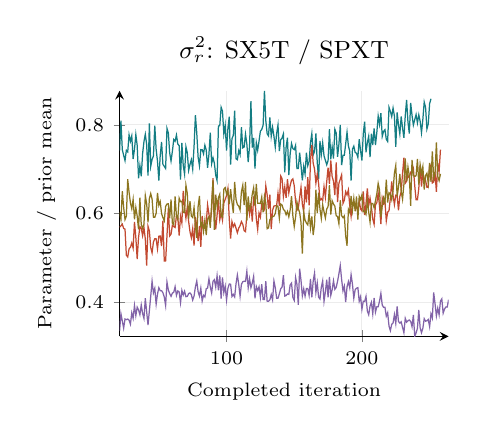
\begin{tikzpicture}
\begin{axis}[width=.475\linewidth,height=4.7cm,title={$\sigma^2_r$: SX5T / SPXT},
 title style={font=\small},xlabel={Completed iteration},ylabel={Parameter / prior mean},
 axis lines=left,grid=major,grid style={gray!15},
 tick label style={font=\scriptsize},label style={font=\scriptsize},scaled ticks=false]
\addplot[chainone,line width=.45pt,no marks] coordinates {(21,0.741627) (22,0.809187) (23,0.743979) (24,0.731318) (25,0.719175) (26,0.742675) (27,0.739117) (28,0.777584) (29,0.762789) (30,0.775163) (31,0.723063) (32,0.744866) (33,0.777869) (34,0.753509) (35,0.67934) (36,0.708219) (37,0.683938) (38,0.734992) (39,0.762296) (40,0.77873) (41,0.755433) (42,0.685333) (43,0.803531) (44,0.706332) (45,0.721908) (46,0.729878) (47,0.798278) (48,0.744635) (49,0.717804) (50,0.67413) (51,0.730932) (52,0.761398) (53,0.710767) (54,0.706464) (55,0.701577) (56,0.792111) (57,0.781922) (58,0.736438) (59,0.718383) (60,0.740341) (61,0.766843) (62,0.762996) (63,0.777048) (64,0.756814) (65,0.753113) (66,0.676533) (67,0.75911) (68,0.708771) (69,0.688765) (70,0.750663) (71,0.73722) (72,0.697188) (73,0.710636) (74,0.721525) (75,0.700168) (76,0.750998) (77,0.822049) (78,0.781564) (79,0.727375) (80,0.707417) (81,0.744091) (82,0.744002) (83,0.734585) (84,0.754027) (85,0.743045) (86,0.703032) (87,0.733902) (88,0.782593) (89,0.712706) (90,0.725766) (91,0.713524) (92,0.686598) (93,0.674295) (94,0.797336) (95,0.798263) (96,0.83955) (97,0.830915) (98,0.779412) (99,0.798947) (100,0.74195) (101,0.791863) (102,0.818577) (103,0.710332) (104,0.768975) (105,0.776351) (106,0.832212) (107,0.723394) (108,0.721351) (109,0.741446) (110,0.732578) (111,0.794617) (112,0.748155) (113,0.7499) (114,0.778969) (115,0.7567) (116,0.715964) (117,0.75221) (118,0.85324) (119,0.748511) (120,0.770266) (121,0.701167) (122,0.759468) (123,0.742599) (124,0.763762) (125,0.785589) (126,0.789596) (127,0.799096) (128,0.876843) (129,0.809484) (130,0.779869) (131,0.775139) (132,0.816528) (133,0.774073) (134,0.794532) (135,0.774592) (136,0.749246) (137,0.780364) (138,0.799748) (139,0.74077) (140,0.766113) (141,0.770419) (142,0.779749) (143,0.692846) (144,0.74929) (145,0.771035) (146,0.686477) (147,0.734834) (148,0.757996) (149,0.746441) (150,0.74406) (151,0.753541) (152,0.701327) (153,0.701327) (154,0.737323) (155,0.708504) (156,0.674581) (157,0.706486) (158,0.68922) (159,0.737438) (160,0.707848) (161,0.717097) (162,0.759175) (163,0.780365) (164,0.732225) (165,0.739864) (166,0.780453) (167,0.714882) (168,0.677246) (169,0.763553) (170,0.732815) (171,0.759361) (172,0.730181) (173,0.720147) (174,0.710064) (175,0.719079) (176,0.790239) (177,0.722411) (178,0.750615) (179,0.724146) (180,0.790075) (181,0.781541) (182,0.727808) (183,0.756021) (184,0.799863) (185,0.70904) (186,0.731391) (187,0.731391) (188,0.757118) (189,0.7834) (190,0.752591) (191,0.740664) (192,0.674216) (193,0.74515) (194,0.751911) (195,0.737746) (196,0.735925) (197,0.726584) (198,0.767473) (199,0.741451) (200,0.719653) (201,0.780163) (202,0.807369) (203,0.738202) (204,0.759678) (205,0.774356) (206,0.727386) (207,0.780054) (208,0.75446) (209,0.792038) (210,0.754184) (211,0.782705) (212,0.819877) (213,0.800947) (214,0.82638) (215,0.773785) (216,0.785184) (217,0.789115) (218,0.767402) (219,0.762443) (220,0.83944) (221,0.830527) (222,0.818622) (223,0.83799) (224,0.819799) (225,0.750126) (226,0.827893) (227,0.800346) (228,0.779049) (229,0.819128) (230,0.792897) (231,0.77082) (232,0.820653) (233,0.856064) (234,0.806487) (235,0.780393) (236,0.849673) (237,0.821439) (238,0.799545) (239,0.811654) (240,0.823226) (241,0.804276) (242,0.822583) (243,0.808076) (244,0.782293) (245,0.812415) (246,0.851585) (247,0.839725) (248,0.79073) (249,0.80207) (250,0.847856) (251,0.858761)};
\addplot[chaintwo,line width=.45pt,no marks] coordinates {(21,0.569203) (22,0.572208) (23,0.576066) (24,0.566429) (25,0.564732) (26,0.505812) (27,0.501965) (28,0.520264) (29,0.523667) (30,0.533544) (31,0.522005) (32,0.581033) (33,0.545939) (34,0.497268) (35,0.54572) (36,0.57013) (37,0.566878) (38,0.549853) (39,0.568204) (40,0.542327) (41,0.482651) (42,0.57108) (43,0.560469) (44,0.523238) (45,0.511425) (46,0.535771) (47,0.543019) (48,0.542795) (49,0.520183) (50,0.548886) (51,0.549045) (52,0.526475) (53,0.583694) (54,0.49293) (55,0.49293) (56,0.54942) (57,0.611444) (58,0.549395) (59,0.553488) (60,0.573428) (61,0.57042) (62,0.56844) (63,0.595749) (64,0.592013) (65,0.550198) (66,0.593752) (67,0.578745) (68,0.651034) (69,0.612699) (70,0.58948) (71,0.614312) (72,0.582086) (73,0.558856) (74,0.545261) (75,0.565948) (76,0.527484) (77,0.592394) (78,0.571013) (79,0.537608) (80,0.571867) (81,0.524677) (82,0.594679) (83,0.566275) (84,0.56765) (85,0.577945) (86,0.619509) (87,0.598908) (88,0.578737) (89,0.608691) (90,0.6795) (91,0.598084) (92,0.564217) (93,0.595834) (94,0.630947) (95,0.585907) (96,0.600955) (97,0.585044) (98,0.623368) (99,0.631953) (100,0.640603) (101,0.656329) (102,0.587524) (103,0.543461) (104,0.58172) (105,0.570199) (106,0.576693) (107,0.566836) (108,0.556531) (109,0.567088) (110,0.572601) (111,0.581667) (112,0.575816) (113,0.561107) (114,0.559032) (115,0.597578) (116,0.618124) (117,0.598417) (118,0.623777) (119,0.581533) (120,0.636591) (121,0.633958) (122,0.588085) (123,0.564013) (124,0.601268) (125,0.591781) (126,0.621463) (127,0.619098) (128,0.610588) (129,0.662265) (130,0.642231) (131,0.60996) (132,0.642518) (133,0.564622) (134,0.607228) (135,0.616813) (136,0.617508) (137,0.617695) (138,0.64588) (139,0.617495) (140,0.684584) (141,0.678825) (142,0.638435) (143,0.660094) (144,0.635509) (145,0.677436) (146,0.646302) (147,0.663171) (148,0.675124) (149,0.678047) (150,0.662916) (151,0.627994) (152,0.607275) (153,0.612334) (154,0.636212) (155,0.659099) (156,0.621104) (157,0.603197) (158,0.660938) (159,0.624914) (160,0.68211) (161,0.61846) (162,0.720036) (163,0.754519) (164,0.713333) (165,0.70033) (166,0.668504) (167,0.689209) (168,0.66766) (169,0.629882) (170,0.633638) (171,0.628968) (172,0.660495) (173,0.636895) (174,0.671941) (175,0.703641) (176,0.666861) (177,0.719704) (178,0.683295) (179,0.672832) (180,0.641628) (181,0.715169) (182,0.62597) (183,0.668185) (184,0.677389) (185,0.687237) (186,0.622692) (187,0.629964) (188,0.649433) (189,0.641895) (190,0.653242) (191,0.618417) (192,0.593686) (193,0.623501) (194,0.619157) (195,0.622604) (196,0.613845) (197,0.606664) (198,0.628809) (199,0.610023) (200,0.606106) (201,0.649638) (202,0.596732) (203,0.621764) (204,0.656833) (205,0.618177) (206,0.634793) (207,0.614803) (208,0.587548) (209,0.575817) (210,0.619622) (211,0.624224) (212,0.646205) (213,0.616708) (214,0.5763) (215,0.634823) (216,0.621776) (217,0.626725) (218,0.583336) (219,0.602877) (220,0.605989) (221,0.634514) (222,0.672282) (223,0.640456) (224,0.62011) (225,0.641308) (226,0.640711) (227,0.607267) (228,0.638439) (229,0.649015) (230,0.690208) (231,0.725787) (232,0.668447) (233,0.672839) (234,0.685947) (235,0.680675) (236,0.69379) (237,0.693793) (238,0.701696) (239,0.66272) (240,0.631007) (241,0.631007) (242,0.6564) (243,0.707867) (244,0.660746) (245,0.692064) (246,0.67858) (247,0.674931) (248,0.659043) (249,0.659593) (250,0.709661) (251,0.708564) (252,0.668926) (253,0.671044) (254,0.691098) (255,0.648904) (256,0.712102) (257,0.694076) (258,0.743995)};
\addplot[chainthree,line width=.45pt,no marks] coordinates {(21,0.335507) (22,0.373766) (23,0.357665) (24,0.341304) (25,0.361927) (26,0.360599) (27,0.361905) (28,0.359471) (29,0.350398) (30,0.375938) (31,0.363771) (32,0.392573) (33,0.369566) (34,0.388758) (35,0.382337) (36,0.371603) (37,0.39361) (38,0.374347) (39,0.3632) (40,0.408766) (41,0.378166) (42,0.34838) (43,0.380677) (44,0.413433) (45,0.447288) (46,0.42091) (47,0.431163) (48,0.39552) (49,0.41822) (50,0.432738) (51,0.425831) (52,0.425874) (53,0.421238) (54,0.411612) (55,0.392275) (56,0.445605) (57,0.427435) (58,0.419363) (59,0.413084) (60,0.420473) (61,0.422189) (62,0.434851) (63,0.41525) (64,0.425338) (65,0.42296) (66,0.398567) (67,0.426645) (68,0.415895) (69,0.424699) (70,0.412404) (71,0.413043) (72,0.41932) (73,0.420823) (74,0.417128) (75,0.404531) (76,0.413792) (77,0.434399) (78,0.447695) (79,0.423377) (80,0.413641) (81,0.431439) (82,0.402465) (83,0.415423) (84,0.411806) (85,0.430519) (86,0.431733) (87,0.452486) (88,0.434361) (89,0.42077) (90,0.446983) (91,0.450567) (92,0.434031) (93,0.459466) (94,0.426912) (95,0.460447) (96,0.40791) (97,0.455659) (98,0.421493) (99,0.436003) (100,0.404752) (101,0.431068) (102,0.440884) (103,0.44051) (104,0.412798) (105,0.417602) (106,0.411745) (107,0.441528) (108,0.461197) (109,0.440287) (110,0.41319) (111,0.440435) (112,0.446267) (113,0.447144) (114,0.446869) (115,0.469669) (116,0.432313) (117,0.452959) (118,0.43259) (119,0.443282) (120,0.458109) (121,0.408494) (122,0.435306) (123,0.426217) (124,0.434652) (125,0.411144) (126,0.440437) (127,0.406036) (128,0.406036) (129,0.447142) (130,0.401796) (131,0.401796) (132,0.405072) (133,0.417305) (134,0.405349) (135,0.44772) (136,0.432811) (137,0.408921) (138,0.408835) (139,0.418729) (140,0.430143) (141,0.43386) (142,0.460687) (143,0.413835) (144,0.41485) (145,0.418528) (146,0.417531) (147,0.438897) (148,0.442944) (149,0.41057) (150,0.403923) (151,0.455583) (152,0.440245) (153,0.394091) (154,0.475376) (155,0.449356) (156,0.414072) (157,0.429858) (158,0.413616) (159,0.430893) (160,0.43066) (161,0.415385) (162,0.452296) (163,0.410652) (164,0.447705) (165,0.465619) (166,0.421973) (167,0.443301) (168,0.411268) (169,0.407158) (170,0.433462) (171,0.44804) (172,0.401958) (173,0.423135) (174,0.450485) (175,0.410956) (176,0.457195) (177,0.415402) (178,0.427818) (179,0.44833) (180,0.428973) (181,0.433353) (182,0.447019) (183,0.463943) (184,0.482719) (185,0.451218) (186,0.425355) (187,0.43621) (188,0.400448) (189,0.434592) (190,0.446431) (191,0.43234) (192,0.461942) (193,0.440513) (194,0.408934) (195,0.428012) (196,0.431384) (197,0.432721) (198,0.402071) (199,0.41227) (200,0.384019) (201,0.402222) (202,0.401461) (203,0.413035) (204,0.380162) (205,0.371657) (206,0.391088) (207,0.399816) (208,0.373608) (209,0.409248) (210,0.377216) (211,0.389552) (212,0.389552) (213,0.402488) (214,0.419756) (215,0.393626) (216,0.388238) (217,0.388399) (218,0.36842) (219,0.376042) (220,0.346138) (221,0.335642) (222,0.349984) (223,0.353038) (224,0.372061) (225,0.351934) (226,0.390115) (227,0.356389) (228,0.352758) (229,0.355544) (230,0.343097) (231,0.331124) (232,0.363639) (233,0.354874) (234,0.358003) (235,0.359782) (236,0.356746) (237,0.344546) (238,0.371164) (239,0.322877) (240,0.330383) (241,0.341055) (242,0.382356) (243,0.342193) (244,0.331058) (245,0.341113) (246,0.36266) (247,0.357083) (248,0.358065) (249,0.360793) (250,0.344726) (251,0.373531) (252,0.36422) (253,0.421808) (254,0.396713) (255,0.368895) (256,0.386342) (257,0.371545) (258,0.402363) (259,0.407352) (260,0.375059) (261,0.384426) (262,0.388972) (263,0.388922) (264,0.405692)};
\addplot[chainfour,line width=.45pt,no marks] coordinates {(21,0.603208) (22,0.586513) (23,0.65011) (24,0.613972) (25,0.586221) (26,0.594007) (27,0.677304) (28,0.647962) (29,0.624159) (30,0.610679) (31,0.63183) (32,0.586779) (33,0.613598) (34,0.594163) (35,0.564217) (36,0.635621) (37,0.575057) (38,0.566152) (39,0.576003) (40,0.640439) (41,0.621758) (42,0.579998) (43,0.633478) (44,0.644948) (45,0.632549) (46,0.591684) (47,0.591684) (48,0.600761) (49,0.646653) (50,0.618634) (51,0.62709) (52,0.59999) (53,0.590807) (54,0.583481) (55,0.615907) (56,0.621458) (57,0.621998) (58,0.589017) (59,0.631497) (60,0.577723) (61,0.574816) (62,0.638548) (63,0.594448) (64,0.586482) (65,0.634535) (66,0.626744) (67,0.627671) (68,0.602866) (69,0.6022) (70,0.663912) (71,0.645435) (72,0.588585) (73,0.627818) (74,0.594341) (75,0.590932) (76,0.613679) (77,0.571738) (78,0.544987) (79,0.615549) (80,0.639867) (81,0.571445) (82,0.579168) (83,0.559122) (84,0.584925) (85,0.551358) (86,0.587724) (87,0.592882) (88,0.567884) (89,0.623476) (90,0.674979) (91,0.562865) (92,0.642713) (93,0.616698) (94,0.635563) (95,0.643459) (96,0.593958) (97,0.591869) (98,0.654988) (99,0.658444) (100,0.643737) (101,0.652378) (102,0.620491) (103,0.655029) (104,0.62558) (105,0.601563) (106,0.671305) (107,0.632046) (108,0.619925) (109,0.616714) (110,0.607913) (111,0.649072) (112,0.663878) (113,0.619258) (114,0.671442) (115,0.583889) (116,0.638581) (117,0.60931) (118,0.619786) (119,0.6438) (120,0.658008) (121,0.61663) (122,0.66662) (123,0.622906) (124,0.623272) (125,0.622463) (126,0.637078) (127,0.602864) (128,0.639194) (129,0.623379) (130,0.565684) (131,0.567647) (132,0.586084) (133,0.589972) (134,0.592721) (135,0.593881) (136,0.600218) (137,0.617769) (138,0.615672) (139,0.589081) (140,0.621337) (141,0.619018) (142,0.60932) (143,0.606523) (144,0.597119) (145,0.604759) (146,0.592475) (147,0.608116) (148,0.639275) (149,0.594527) (150,0.57043) (151,0.591687) (152,0.625685) (153,0.611072) (154,0.602089) (155,0.580146) (156,0.50963) (157,0.602316) (158,0.585174) (159,0.57846) (160,0.574303) (161,0.601546) (162,0.567481) (163,0.593502) (164,0.551297) (165,0.575487) (166,0.653607) (167,0.600784) (168,0.646737) (169,0.610284) (170,0.588985) (171,0.619755) (172,0.603904) (173,0.589879) (174,0.610072) (175,0.615525) (176,0.664115) (177,0.597504) (178,0.628881) (179,0.621369) (180,0.616548) (181,0.59515) (182,0.593079) (183,0.577041) (184,0.629789) (185,0.595129) (186,0.590611) (187,0.594581) (188,0.54956) (189,0.526978) (190,0.609529) (191,0.602438) (192,0.63942) (193,0.607) (194,0.634095) (195,0.604914) (196,0.63874) (197,0.586334) (198,0.638673) (199,0.631219) (200,0.641935) (201,0.603963) (202,0.605221) (203,0.598275) (204,0.629069) (205,0.60343) (206,0.580526) (207,0.62256) (208,0.62256) (209,0.612865) (210,0.629022) (211,0.644567) (212,0.668052) (213,0.652992) (214,0.592644) (215,0.617075) (216,0.635382) (217,0.624259) (218,0.676215) (219,0.624533) (220,0.646737) (221,0.643174) (222,0.631041) (223,0.65215) (224,0.691166) (225,0.708344) (226,0.638586) (227,0.659733) (228,0.689183) (229,0.650159) (230,0.632233) (231,0.66599) (232,0.724061) (233,0.672759) (234,0.704672) (235,0.684254) (236,0.617421) (237,0.721135) (238,0.685571) (239,0.683382) (240,0.685403) (241,0.72325) (242,0.665308) (243,0.710409) (244,0.689952) (245,0.705889) (246,0.654044) (247,0.685451) (248,0.690852) (249,0.668492) (250,0.714131) (251,0.671409) (252,0.740309) (253,0.679424) (254,0.689596) (255,0.760538) (256,0.684225) (257,0.674115) (258,0.689435)};
\end{axis}\end{tikzpicture}
\par\smallskip
\textbf{Should the prior and posterior match?} There is no requirement that they match,
or that every posterior must be narrower. Similarity can mean weak information about a
parameter or agreement with the prior. A shift may reflect learning, prior conflict, or
sampling problems; its interpretation requires diagnostics and sensitivity checks.

\textbf{Before treating draw percentiles as credible intervals:} the repository's target
is four independent chains, rank-normalized split/folded $\widehat R<1.01$, bulk and tail
ESS at least 400, and mean MCSE/posterior-SD at most 0.05 for reported quantities [4].
The saved diagnostic record contains no usable values for these metrics. The 20-iteration
burn-in setting is a retention rule, not evidence that warm-up was sufficient. Passing
diagnostics would still leave prior sensitivity and model adequacy to assess.

\clearpage
\section*{7. Initial-state priors and reproducibility}
The following centers come from the reserved first 104 weekly returns.
The $B_1$ entries are percentage points of weekly expected return; its prior SD is
$2\sqrt{\bar V_{B,jj}}$. The log-variance centers use percentage-return units.
\begin{center}\small
\begin{tabular}{lrrr}\toprule
Series & $\bar B_j$ & Prior SD of $B_{j1}$ & $\bar h_j$\\\midrule
AUDUSD & 0.1567 & 0.2993 & 0.8452 \\
BCOMCOT & 0.8553 & 0.8258 & 2.8753 \\
BCOMGCTR & 0.1873 & 0.3776 & 1.3105 \\
EURUSD & 0.0854 & 0.2618 & 0.5778 \\
GBPUSD & 0.1003 & 0.2405 & 0.4082 \\
I02981JP & 0.0061 & 0.0639 & -2.2428 \\
LEATTREU & 0.1109 & 0.0846 & -1.6824 \\
LSG1TRGU & 0.0880 & 0.1122 & -1.1168 \\
LUATTRUU & 0.0656 & 0.1124 & -1.1128 \\
NKYTR & 0.2423 & 0.4541 & 1.6793 \\
SPXT & 0.2518 & 0.2849 & 0.7470 \\
SX5T & 0.3214 & 0.3427 & 1.1163 \\
TUKXG & 0.3055 & 0.2423 & 0.4226 \\
USDJPY & -0.0595 & 0.2421 & 0.4216 \\
\bottomrule\end{tabular}\end{center}
The $B_1$ prior is multivariate, with covariance $4\bar V_B$, not 14 independent normals.
For $h_1$ and $r_1$, the marginal priors follow the Student-$t$ expression on page 2.
For $P_{ij,t}$ there is an induced joint prior obtained by mapping the entire $r_t$ vector;
assigning independent priors to ordinary pairwise correlations would change this model.

\textbf{Fixed-parameter smoothing is a different output.} When
\texttt{estimate\_parameters=false}, the workflow uses saved parameter means or saved
parameter draws while updating latent states. This is not a new estimation of
$p(\theta\mid y)$. Holding means fixed excludes parameter uncertainty; reusing saved
draws includes their variation but does not reweight them into an updated parameter
posterior when new observations arrive.

\textbf{Saved evidence.} Parameter file, estimated at 2026-09-27T09:08:55.845Z:
\par{\footnotesize\nolinkurl{parameters_<run-id>.mat}}
\par Run: {\footnotesize\nolinkurl{20260926-230854-651-chain1-w20-r500-thin1/estimation}}.
\par Source SHA-256: {\scriptsize\nolinkurl{f11259e4c6347a54204cecb4f5ac3363c06ef2b05f787ab33ed9ab99e04c5bd7}}.
The companion numerical CSV contains prior moments and retained-draw means and quantiles
for all 210 parameters. Its manifest records file hashes, chain counts, and validation
of positive definiteness, draw counts, and agreement with the saved parameter means.

\textbf{Implementation sources.}\par
{\footnotesize\begin{tabular}{@{}ll@{}}
\nolinkurl{toolbox/dsc_calibrate_priors.m} & Defines the priors\\
\nolinkurl{toolbox/dsc_prepare_inference.m} & Splits calibration and likelihood dates\\
\nolinkurl{toolbox/dsc_sample.m} & Implements the posterior updates\\
\nolinkurl{toolbox/dsc_save_parameters.m} & Preserves draws and chain IDs\\
\end{tabular}}
\par The generated LaTeX is self-contained and has no external figure dependencies.

\textbf{Methodological references.}\par
{\footnotesize
[1] Archakov and Hansen (2021). \emph{A New Parametrization of Correlation Matrices}.
\href{https://arxiv.org/abs/2012.02395}{Paper and reconstruction method}.\par
[2] MathWorks. \emph{iwishrnd}: inverse-Wishart parameterization and expectation.
\href{https://www.mathworks.com/help/stats/iwishrnd.html}{Official documentation}.\par
[3] Murray, Adams and MacKay (2010). \emph{Elliptical Slice Sampling}.
\href{https://proceedings.mlr.press/v9/murray10a.html}{PMLR 9, 541--548}.\par
[4] Vehtari et al. (2021). \emph{Rank-Normalization, Folding, and Localization}.
\href{https://arxiv.org/abs/1903.08008}{Bayesian Analysis 16, 667--718}.
}
\clearpage\section*{Mean-evolution variances and volatility-evolution variances}

\small All rows use the same saved run. Prior moments are analytical.
The last three columns are empirical retained-draw summaries; convergence is unverified.
Intervals are marginal 5th--95th percentiles, not simultaneous intervals.
Ticker labels omit only the common ``Index'' suffix.
\par\medskip
\begingroup\fontsize{7.8}{10.5}\selectfont\setlength{\tabcolsep}{3pt}
\renewcommand{\arraystretch}{1.45}
\begin{tabular*}{\linewidth}{@{\extracolsep{\fill}}lrrrrr@{}}
\toprule
Parameter & Prior mean & Prior SD & Draw median & Draw 5\% & Draw 95\%\\
\midrule
V(AUDUSD,AUDUSD) & $2.616\times10^{-6}$ & $3.967\times10^{-7}$ & $2.711\times10^{-6}$ & $2.126\times10^{-6}$ & $3.352\times10^{-6}$ \\
V(BCOMCOT,BCOMCOT) & $1.992\times10^{-5}$ & $3.021\times10^{-6}$ & $1.982\times10^{-5}$ & $1.561\times10^{-5}$ & $2.433\times10^{-5}$ \\
V(BCOMGCTR,BCOMGCTR) & $4.166\times10^{-6}$ & $6.317\times10^{-7}$ & $4.271\times10^{-6}$ & $3.421\times10^{-6}$ & $5.322\times10^{-6}$ \\
V(EURUSD,EURUSD) & $2.002\times10^{-6}$ & $3.036\times10^{-7}$ & $2.070\times10^{-6}$ & $1.676\times10^{-6}$ & $2.582\times10^{-6}$ \\
V(GBPUSD,GBPUSD) & $1.690\times10^{-6}$ & $2.562\times10^{-7}$ & $1.678\times10^{-6}$ & $1.365\times10^{-6}$ & $2.087\times10^{-6}$ \\
V(I02981JP,I02981JP) & $1.193\times10^{-7}$ & $1.809\times10^{-8}$ & $1.195\times10^{-7}$ & $9.369\times10^{-8}$ & $1.602\times10^{-7}$ \\
V(LEATTREU,LEATTREU) & $2.089\times10^{-7}$ & $3.167\times10^{-8}$ & $2.103\times10^{-7}$ & $1.682\times10^{-7}$ & $2.785\times10^{-7}$ \\
V(LSG1TRGU,LSG1TRGU) & $3.678\times10^{-7}$ & $5.577\times10^{-8}$ & $3.673\times10^{-7}$ & $2.900\times10^{-7}$ & $4.827\times10^{-7}$ \\
V(LUATTRUU,LUATTRUU) & $3.692\times10^{-7}$ & $5.598\times10^{-8}$ & $3.851\times10^{-7}$ & $2.956\times10^{-7}$ & $4.892\times10^{-7}$ \\
V(NKYTR,NKYTR) & $6.024\times10^{-6}$ & $9.134\times10^{-7}$ & $5.886\times10^{-6}$ & $4.744\times10^{-6}$ & $7.297\times10^{-6}$ \\
V(SPXT,SPXT) & $2.372\times10^{-6}$ & $3.596\times10^{-7}$ & $2.349\times10^{-6}$ & $1.830\times10^{-6}$ & $2.868\times10^{-6}$ \\
V(SX5T,SX5T) & $3.431\times10^{-6}$ & $5.202\times10^{-7}$ & $3.344\times10^{-6}$ & $2.665\times10^{-6}$ & $4.315\times10^{-6}$ \\
V(TUKXG,TUKXG) & $1.715\times10^{-6}$ & $2.600\times10^{-7}$ & $1.665\times10^{-6}$ & $1.322\times10^{-6}$ & $2.065\times10^{-6}$ \\
V(USDJPY,USDJPY) & $1.713\times10^{-6}$ & $2.597\times10^{-7}$ & $1.762\times10^{-6}$ & $1.375\times10^{-6}$ & $2.323\times10^{-6}$ \\
h(AUDUSD) & $1.094\times10^{-3}$ & $3.868\times10^{-4}$ & $2.563\times10^{-4}$ & $1.718\times10^{-4}$ & $5.996\times10^{-4}$ \\
h(BCOMCOT) & $1.094\times10^{-3}$ & $3.868\times10^{-4}$ & $4.261\times10^{-4}$ & $1.978\times10^{-4}$ & $9.935\times10^{-4}$ \\
h(BCOMGCTR) & $1.094\times10^{-3}$ & $3.868\times10^{-4}$ & $4.070\times10^{-4}$ & $2.426\times10^{-4}$ & $1.034\times10^{-3}$ \\
h(EURUSD) & $1.094\times10^{-3}$ & $3.868\times10^{-4}$ & $6.085\times10^{-4}$ & $2.072\times10^{-4}$ & $1.092\times10^{-3}$ \\
h(GBPUSD) & $1.094\times10^{-3}$ & $3.868\times10^{-4}$ & $1.815\times10^{-4}$ & $9.270\times10^{-5}$ & $4.819\times10^{-4}$ \\
h(I02981JP) & $1.094\times10^{-3}$ & $3.868\times10^{-4}$ & $5.673\times10^{-4}$ & $2.052\times10^{-4}$ & $1.073\times10^{-3}$ \\
h(LEATTREU) & $1.094\times10^{-3}$ & $3.868\times10^{-4}$ & $6.006\times10^{-4}$ & $2.771\times10^{-4}$ & $9.441\times10^{-4}$ \\
h(LSG1TRGU) & $1.094\times10^{-3}$ & $3.868\times10^{-4}$ & $4.814\times10^{-4}$ & $2.229\times10^{-4}$ & $1.303\times10^{-3}$ \\
h(LUATTRUU) & $1.094\times10^{-3}$ & $3.868\times10^{-4}$ & $3.126\times10^{-4}$ & $1.640\times10^{-4}$ & $5.854\times10^{-4}$ \\
h(NKYTR) & $1.094\times10^{-3}$ & $3.868\times10^{-4}$ & $2.895\times10^{-4}$ & $1.318\times10^{-4}$ & $6.310\times10^{-4}$ \\
h(SPXT) & $1.094\times10^{-3}$ & $3.868\times10^{-4}$ & $6.486\times10^{-4}$ & $2.086\times10^{-4}$ & $8.986\times10^{-4}$ \\
h(SX5T) & $1.094\times10^{-3}$ & $3.868\times10^{-4}$ & $4.128\times10^{-4}$ & $2.993\times10^{-4}$ & $7.788\times10^{-4}$ \\
h(TUKXG) & $1.094\times10^{-3}$ & $3.868\times10^{-4}$ & $4.924\times10^{-4}$ & $2.825\times10^{-4}$ & $1.072\times10^{-3}$ \\
h(USDJPY) & $1.094\times10^{-3}$ & $3.868\times10^{-4}$ & $8.206\times10^{-4}$ & $3.353\times10^{-4}$ & $1.249\times10^{-3}$ \\
\bottomrule
\end{tabular*}\endgroup
\par\medskip\footnotesize
V(i,j) describes covariance of changes in expected returns, in squared percentage-point units.
h(j) denotes $\sigma_{h,j}^{2}$; r(i,j) denotes $\sigma_{r,k}^{2}$ for the matrix-log coordinate
associated with that pair. Neither r(i,j) nor V(i,j) is a return correlation.

\clearpage\section*{Correlation-coordinate evolution variances: 1--31}

\small All rows use the same saved run. Prior moments are analytical.
The last three columns are empirical retained-draw summaries; convergence is unverified.
Intervals are marginal 5th--95th percentiles, not simultaneous intervals.
Ticker labels omit only the common ``Index'' suffix.
\par\medskip
\begingroup\fontsize{7.8}{10.5}\selectfont\setlength{\tabcolsep}{3pt}
\renewcommand{\arraystretch}{1.45}
\begin{tabular*}{\linewidth}{@{\extracolsep{\fill}}lrrrrr@{}}
\toprule
Parameter & Prior mean & Prior SD & Draw median & Draw 5\% & Draw 95\%\\
\midrule
r(BCOMCOT,AUDUSD) & $2.381\times10^{-4}$ & $8.418\times10^{-5}$ & $7.210\times10^{-5}$ & $3.858\times10^{-5}$ & $1.215\times10^{-4}$ \\
r(BCOMGCTR,AUDUSD) & $2.381\times10^{-4}$ & $8.418\times10^{-5}$ & $9.311\times10^{-5}$ & $4.071\times10^{-5}$ & $1.843\times10^{-4}$ \\
r(EURUSD,AUDUSD) & $2.381\times10^{-4}$ & $8.418\times10^{-5}$ & $7.941\times10^{-5}$ & $4.949\times10^{-5}$ & $1.177\times10^{-4}$ \\
r(GBPUSD,AUDUSD) & $2.381\times10^{-4}$ & $8.418\times10^{-5}$ & $1.058\times10^{-4}$ & $6.456\times10^{-5}$ & $1.650\times10^{-4}$ \\
r(I02981JP,AUDUSD) & $2.381\times10^{-4}$ & $8.418\times10^{-5}$ & $7.898\times10^{-5}$ & $4.445\times10^{-5}$ & $1.053\times10^{-4}$ \\
r(LEATTREU,AUDUSD) & $2.381\times10^{-4}$ & $8.418\times10^{-5}$ & $1.214\times10^{-4}$ & $4.954\times10^{-5}$ & $1.877\times10^{-4}$ \\
r(LSG1TRGU,AUDUSD) & $2.381\times10^{-4}$ & $8.418\times10^{-5}$ & $7.803\times10^{-5}$ & $4.005\times10^{-5}$ & $1.161\times10^{-4}$ \\
r(LUATTRUU,AUDUSD) & $2.381\times10^{-4}$ & $8.418\times10^{-5}$ & $8.297\times10^{-5}$ & $4.644\times10^{-5}$ & $1.767\times10^{-4}$ \\
r(NKYTR,AUDUSD) & $2.381\times10^{-4}$ & $8.418\times10^{-5}$ & $7.064\times10^{-5}$ & $3.167\times10^{-5}$ & $9.763\times10^{-5}$ \\
r(SPXT,AUDUSD) & $2.381\times10^{-4}$ & $8.418\times10^{-5}$ & $1.625\times10^{-4}$ & $4.433\times10^{-5}$ & $3.964\times10^{-4}$ \\
r(SX5T,AUDUSD) & $2.381\times10^{-4}$ & $8.418\times10^{-5}$ & $1.163\times10^{-4}$ & $4.852\times10^{-5}$ & $1.861\times10^{-4}$ \\
r(TUKXG,AUDUSD) & $2.381\times10^{-4}$ & $8.418\times10^{-5}$ & $1.164\times10^{-4}$ & $6.985\times10^{-5}$ & $1.315\times10^{-4}$ \\
r(USDJPY,AUDUSD) & $2.381\times10^{-4}$ & $8.418\times10^{-5}$ & $1.441\times10^{-4}$ & $1.061\times10^{-4}$ & $1.849\times10^{-4}$ \\
r(BCOMGCTR,BCOMCOT) & $2.381\times10^{-4}$ & $8.418\times10^{-5}$ & $7.257\times10^{-5}$ & $3.788\times10^{-5}$ & $1.187\times10^{-4}$ \\
r(EURUSD,BCOMCOT) & $2.381\times10^{-4}$ & $8.418\times10^{-5}$ & $9.664\times10^{-5}$ & $4.494\times10^{-5}$ & $1.796\times10^{-4}$ \\
r(GBPUSD,BCOMCOT) & $2.381\times10^{-4}$ & $8.418\times10^{-5}$ & $8.811\times10^{-5}$ & $3.328\times10^{-5}$ & $1.107\times10^{-4}$ \\
r(I02981JP,BCOMCOT) & $2.381\times10^{-4}$ & $8.418\times10^{-5}$ & $8.414\times10^{-5}$ & $4.692\times10^{-5}$ & $1.210\times10^{-4}$ \\
r(LEATTREU,BCOMCOT) & $2.381\times10^{-4}$ & $8.418\times10^{-5}$ & $8.460\times10^{-5}$ & $4.079\times10^{-5}$ & $1.126\times10^{-4}$ \\
r(LSG1TRGU,BCOMCOT) & $2.381\times10^{-4}$ & $8.418\times10^{-5}$ & $1.197\times10^{-4}$ & $7.899\times10^{-5}$ & $1.475\times10^{-4}$ \\
r(LUATTRUU,BCOMCOT) & $2.381\times10^{-4}$ & $8.418\times10^{-5}$ & $1.359\times10^{-4}$ & $5.184\times10^{-5}$ & $1.905\times10^{-4}$ \\
r(NKYTR,BCOMCOT) & $2.381\times10^{-4}$ & $8.418\times10^{-5}$ & $6.757\times10^{-5}$ & $3.803\times10^{-5}$ & $1.083\times10^{-4}$ \\
r(SPXT,BCOMCOT) & $2.381\times10^{-4}$ & $8.418\times10^{-5}$ & $1.729\times10^{-4}$ & $1.280\times10^{-4}$ & $3.744\times10^{-4}$ \\
r(SX5T,BCOMCOT) & $2.381\times10^{-4}$ & $8.418\times10^{-5}$ & $8.058\times10^{-5}$ & $2.877\times10^{-5}$ & $1.613\times10^{-4}$ \\
r(TUKXG,BCOMCOT) & $2.381\times10^{-4}$ & $8.418\times10^{-5}$ & $8.809\times10^{-5}$ & $3.488\times10^{-5}$ & $1.277\times10^{-4}$ \\
r(USDJPY,BCOMCOT) & $2.381\times10^{-4}$ & $8.418\times10^{-5}$ & $7.041\times10^{-5}$ & $3.953\times10^{-5}$ & $1.816\times10^{-4}$ \\
r(EURUSD,BCOMGCTR) & $2.381\times10^{-4}$ & $8.418\times10^{-5}$ & $1.557\times10^{-4}$ & $5.210\times10^{-5}$ & $2.285\times10^{-4}$ \\
r(GBPUSD,BCOMGCTR) & $2.381\times10^{-4}$ & $8.418\times10^{-5}$ & $5.844\times10^{-5}$ & $2.875\times10^{-5}$ & $1.153\times10^{-4}$ \\
r(I02981JP,BCOMGCTR) & $2.381\times10^{-4}$ & $8.418\times10^{-5}$ & $7.230\times10^{-5}$ & $3.703\times10^{-5}$ & $9.722\times10^{-5}$ \\
r(LEATTREU,BCOMGCTR) & $2.381\times10^{-4}$ & $8.418\times10^{-5}$ & $8.622\times10^{-5}$ & $4.665\times10^{-5}$ & $1.038\times10^{-4}$ \\
r(LSG1TRGU,BCOMGCTR) & $2.381\times10^{-4}$ & $8.418\times10^{-5}$ & $7.485\times10^{-5}$ & $3.127\times10^{-5}$ & $1.650\times10^{-4}$ \\
r(LUATTRUU,BCOMGCTR) & $2.381\times10^{-4}$ & $8.418\times10^{-5}$ & $7.079\times10^{-5}$ & $3.704\times10^{-5}$ & $1.023\times10^{-4}$ \\
\bottomrule
\end{tabular*}\endgroup
\par\medskip\footnotesize
V(i,j) describes covariance of changes in expected returns, in squared percentage-point units.
h(j) denotes $\sigma_{h,j}^{2}$; r(i,j) denotes $\sigma_{r,k}^{2}$ for the matrix-log coordinate
associated with that pair. Neither r(i,j) nor V(i,j) is a return correlation.

\clearpage\section*{Correlation-coordinate evolution variances: 32--62}

\small All rows use the same saved run. Prior moments are analytical.
The last three columns are empirical retained-draw summaries; convergence is unverified.
Intervals are marginal 5th--95th percentiles, not simultaneous intervals.
Ticker labels omit only the common ``Index'' suffix.
\par\medskip
\begingroup\fontsize{7.8}{10.5}\selectfont\setlength{\tabcolsep}{3pt}
\renewcommand{\arraystretch}{1.45}
\begin{tabular*}{\linewidth}{@{\extracolsep{\fill}}lrrrrr@{}}
\toprule
Parameter & Prior mean & Prior SD & Draw median & Draw 5\% & Draw 95\%\\
\midrule
r(NKYTR,BCOMGCTR) & $2.381\times10^{-4}$ & $8.418\times10^{-5}$ & $7.867\times10^{-5}$ & $3.743\times10^{-5}$ & $1.447\times10^{-4}$ \\
r(SPXT,BCOMGCTR) & $2.381\times10^{-4}$ & $8.418\times10^{-5}$ & $6.517\times10^{-5}$ & $3.409\times10^{-5}$ & $8.672\times10^{-5}$ \\
r(SX5T,BCOMGCTR) & $2.381\times10^{-4}$ & $8.418\times10^{-5}$ & $7.917\times10^{-5}$ & $4.143\times10^{-5}$ & $1.383\times10^{-4}$ \\
r(TUKXG,BCOMGCTR) & $2.381\times10^{-4}$ & $8.418\times10^{-5}$ & $1.962\times10^{-4}$ & $4.067\times10^{-5}$ & $2.692\times10^{-4}$ \\
r(USDJPY,BCOMGCTR) & $2.381\times10^{-4}$ & $8.418\times10^{-5}$ & $7.348\times10^{-5}$ & $3.549\times10^{-5}$ & $2.047\times10^{-4}$ \\
r(GBPUSD,EURUSD) & $2.381\times10^{-4}$ & $8.418\times10^{-5}$ & $7.277\times10^{-5}$ & $3.072\times10^{-5}$ & $1.306\times10^{-4}$ \\
r(I02981JP,EURUSD) & $2.381\times10^{-4}$ & $8.418\times10^{-5}$ & $9.417\times10^{-5}$ & $4.656\times10^{-5}$ & $1.249\times10^{-4}$ \\
r(LEATTREU,EURUSD) & $2.381\times10^{-4}$ & $8.418\times10^{-5}$ & $8.373\times10^{-5}$ & $3.204\times10^{-5}$ & $1.192\times10^{-4}$ \\
r(LSG1TRGU,EURUSD) & $2.381\times10^{-4}$ & $8.418\times10^{-5}$ & $6.958\times10^{-5}$ & $3.351\times10^{-5}$ & $1.129\times10^{-4}$ \\
r(LUATTRUU,EURUSD) & $2.381\times10^{-4}$ & $8.418\times10^{-5}$ & $8.715\times10^{-5}$ & $4.701\times10^{-5}$ & $2.306\times10^{-4}$ \\
r(NKYTR,EURUSD) & $2.381\times10^{-4}$ & $8.418\times10^{-5}$ & $8.678\times10^{-5}$ & $5.284\times10^{-5}$ & $1.496\times10^{-4}$ \\
r(SPXT,EURUSD) & $2.381\times10^{-4}$ & $8.418\times10^{-5}$ & $1.432\times10^{-4}$ & $4.140\times10^{-5}$ & $2.130\times10^{-4}$ \\
r(SX5T,EURUSD) & $2.381\times10^{-4}$ & $8.418\times10^{-5}$ & $5.995\times10^{-5}$ & $3.006\times10^{-5}$ & $9.041\times10^{-5}$ \\
r(TUKXG,EURUSD) & $2.381\times10^{-4}$ & $8.418\times10^{-5}$ & $6.982\times10^{-5}$ & $3.613\times10^{-5}$ & $9.803\times10^{-5}$ \\
r(USDJPY,EURUSD) & $2.381\times10^{-4}$ & $8.418\times10^{-5}$ & $7.901\times10^{-5}$ & $3.410\times10^{-5}$ & $2.577\times10^{-4}$ \\
r(I02981JP,GBPUSD) & $2.381\times10^{-4}$ & $8.418\times10^{-5}$ & $7.307\times10^{-5}$ & $4.919\times10^{-5}$ & $1.056\times10^{-4}$ \\
r(LEATTREU,GBPUSD) & $2.381\times10^{-4}$ & $8.418\times10^{-5}$ & $7.223\times10^{-5}$ & $3.448\times10^{-5}$ & $1.802\times10^{-4}$ \\
r(LSG1TRGU,GBPUSD) & $2.381\times10^{-4}$ & $8.418\times10^{-5}$ & $6.943\times10^{-5}$ & $3.592\times10^{-5}$ & $1.024\times10^{-4}$ \\
r(LUATTRUU,GBPUSD) & $2.381\times10^{-4}$ & $8.418\times10^{-5}$ & $7.593\times10^{-5}$ & $4.152\times10^{-5}$ & $2.728\times10^{-4}$ \\
r(NKYTR,GBPUSD) & $2.381\times10^{-4}$ & $8.418\times10^{-5}$ & $1.753\times10^{-4}$ & $4.736\times10^{-5}$ & $4.452\times10^{-4}$ \\
r(SPXT,GBPUSD) & $2.381\times10^{-4}$ & $8.418\times10^{-5}$ & $9.080\times10^{-5}$ & $5.496\times10^{-5}$ & $2.126\times10^{-4}$ \\
r(SX5T,GBPUSD) & $2.381\times10^{-4}$ & $8.418\times10^{-5}$ & $8.453\times10^{-5}$ & $4.596\times10^{-5}$ & $2.236\times10^{-4}$ \\
r(TUKXG,GBPUSD) & $2.381\times10^{-4}$ & $8.418\times10^{-5}$ & $7.014\times10^{-5}$ & $3.937\times10^{-5}$ & $1.206\times10^{-4}$ \\
r(USDJPY,GBPUSD) & $2.381\times10^{-4}$ & $8.418\times10^{-5}$ & $1.296\times10^{-4}$ & $9.953\times10^{-5}$ & $1.527\times10^{-4}$ \\
r(LEATTREU,I02981JP) & $2.381\times10^{-4}$ & $8.418\times10^{-5}$ & $8.404\times10^{-5}$ & $3.892\times10^{-5}$ & $1.265\times10^{-4}$ \\
r(LSG1TRGU,I02981JP) & $2.381\times10^{-4}$ & $8.418\times10^{-5}$ & $6.385\times10^{-5}$ & $3.139\times10^{-5}$ & $9.797\times10^{-5}$ \\
r(LUATTRUU,I02981JP) & $2.381\times10^{-4}$ & $8.418\times10^{-5}$ & $8.499\times10^{-5}$ & $3.178\times10^{-5}$ & $1.954\times10^{-4}$ \\
r(NKYTR,I02981JP) & $2.381\times10^{-4}$ & $8.418\times10^{-5}$ & $1.629\times10^{-4}$ & $7.326\times10^{-5}$ & $2.723\times10^{-4}$ \\
r(SPXT,I02981JP) & $2.381\times10^{-4}$ & $8.418\times10^{-5}$ & $1.910\times10^{-4}$ & $5.715\times10^{-5}$ & $3.557\times10^{-4}$ \\
r(SX5T,I02981JP) & $2.381\times10^{-4}$ & $8.418\times10^{-5}$ & $8.153\times10^{-5}$ & $4.280\times10^{-5}$ & $9.892\times10^{-5}$ \\
r(TUKXG,I02981JP) & $2.381\times10^{-4}$ & $8.418\times10^{-5}$ & $7.064\times10^{-5}$ & $3.492\times10^{-5}$ & $1.256\times10^{-4}$ \\
\bottomrule
\end{tabular*}\endgroup
\par\medskip\footnotesize
V(i,j) describes covariance of changes in expected returns, in squared percentage-point units.
h(j) denotes $\sigma_{h,j}^{2}$; r(i,j) denotes $\sigma_{r,k}^{2}$ for the matrix-log coordinate
associated with that pair. Neither r(i,j) nor V(i,j) is a return correlation.

\clearpage\section*{Correlation-coordinate evolution variances: 63--91}

\small All rows use the same saved run. Prior moments are analytical.
The last three columns are empirical retained-draw summaries; convergence is unverified.
Intervals are marginal 5th--95th percentiles, not simultaneous intervals.
Ticker labels omit only the common ``Index'' suffix.
\par\medskip
\begingroup\fontsize{7.8}{10.5}\selectfont\setlength{\tabcolsep}{3pt}
\renewcommand{\arraystretch}{1.45}
\begin{tabular*}{\linewidth}{@{\extracolsep{\fill}}lrrrrr@{}}
\toprule
Parameter & Prior mean & Prior SD & Draw median & Draw 5\% & Draw 95\%\\
\midrule
r(USDJPY,I02981JP) & $2.381\times10^{-4}$ & $8.418\times10^{-5}$ & $7.389\times10^{-5}$ & $4.249\times10^{-5}$ & $1.074\times10^{-4}$ \\
r(LSG1TRGU,LEATTREU) & $2.381\times10^{-4}$ & $8.418\times10^{-5}$ & $7.885\times10^{-5}$ & $2.685\times10^{-5}$ & $1.609\times10^{-4}$ \\
r(LUATTRUU,LEATTREU) & $2.381\times10^{-4}$ & $8.418\times10^{-5}$ & $1.003\times10^{-4}$ & $4.283\times10^{-5}$ & $1.895\times10^{-4}$ \\
r(NKYTR,LEATTREU) & $2.381\times10^{-4}$ & $8.418\times10^{-5}$ & $1.096\times10^{-4}$ & $8.115\times10^{-5}$ & $1.329\times10^{-4}$ \\
r(SPXT,LEATTREU) & $2.381\times10^{-4}$ & $8.418\times10^{-5}$ & $1.166\times10^{-4}$ & $3.763\times10^{-5}$ & $1.631\times10^{-4}$ \\
r(SX5T,LEATTREU) & $2.381\times10^{-4}$ & $8.418\times10^{-5}$ & $7.585\times10^{-5}$ & $4.013\times10^{-5}$ & $1.233\times10^{-4}$ \\
r(TUKXG,LEATTREU) & $2.381\times10^{-4}$ & $8.418\times10^{-5}$ & $1.538\times10^{-4}$ & $6.964\times10^{-5}$ & $3.654\times10^{-4}$ \\
r(USDJPY,LEATTREU) & $2.381\times10^{-4}$ & $8.418\times10^{-5}$ & $7.045\times10^{-5}$ & $3.373\times10^{-5}$ & $1.139\times10^{-4}$ \\
r(LUATTRUU,LSG1TRGU) & $2.381\times10^{-4}$ & $8.418\times10^{-5}$ & $1.042\times10^{-4}$ & $4.782\times10^{-5}$ & $2.029\times10^{-4}$ \\
r(NKYTR,LSG1TRGU) & $2.381\times10^{-4}$ & $8.418\times10^{-5}$ & $6.295\times10^{-5}$ & $3.825\times10^{-5}$ & $1.048\times10^{-4}$ \\
r(SPXT,LSG1TRGU) & $2.381\times10^{-4}$ & $8.418\times10^{-5}$ & $1.061\times10^{-4}$ & $2.742\times10^{-5}$ & $1.502\times10^{-4}$ \\
r(SX5T,LSG1TRGU) & $2.381\times10^{-4}$ & $8.418\times10^{-5}$ & $7.337\times10^{-5}$ & $4.337\times10^{-5}$ & $1.065\times10^{-4}$ \\
r(TUKXG,LSG1TRGU) & $2.381\times10^{-4}$ & $8.418\times10^{-5}$ & $6.854\times10^{-5}$ & $2.678\times10^{-5}$ & $1.089\times10^{-4}$ \\
r(USDJPY,LSG1TRGU) & $2.381\times10^{-4}$ & $8.418\times10^{-5}$ & $8.565\times10^{-5}$ & $4.076\times10^{-5}$ & $1.514\times10^{-4}$ \\
r(NKYTR,LUATTRUU) & $2.381\times10^{-4}$ & $8.418\times10^{-5}$ & $8.236\times10^{-5}$ & $5.160\times10^{-5}$ & $2.665\times10^{-4}$ \\
r(SPXT,LUATTRUU) & $2.381\times10^{-4}$ & $8.418\times10^{-5}$ & $6.787\times10^{-5}$ & $3.737\times10^{-5}$ & $1.054\times10^{-4}$ \\
r(SX5T,LUATTRUU) & $2.381\times10^{-4}$ & $8.418\times10^{-5}$ & $1.029\times10^{-4}$ & $5.068\times10^{-5}$ & $1.792\times10^{-4}$ \\
r(TUKXG,LUATTRUU) & $2.381\times10^{-4}$ & $8.418\times10^{-5}$ & $1.472\times10^{-4}$ & $6.291\times10^{-5}$ & $3.718\times10^{-4}$ \\
r(USDJPY,LUATTRUU) & $2.381\times10^{-4}$ & $8.418\times10^{-5}$ & $7.537\times10^{-5}$ & $3.983\times10^{-5}$ & $2.055\times10^{-4}$ \\
r(SPXT,NKYTR) & $2.381\times10^{-4}$ & $8.418\times10^{-5}$ & $7.147\times10^{-5}$ & $3.337\times10^{-5}$ & $2.723\times10^{-4}$ \\
r(SX5T,NKYTR) & $2.381\times10^{-4}$ & $8.418\times10^{-5}$ & $1.312\times10^{-4}$ & $4.065\times10^{-5}$ & $2.842\times10^{-4}$ \\
r(TUKXG,NKYTR) & $2.381\times10^{-4}$ & $8.418\times10^{-5}$ & $1.195\times10^{-4}$ & $6.680\times10^{-5}$ & $1.642\times10^{-4}$ \\
r(USDJPY,NKYTR) & $2.381\times10^{-4}$ & $8.418\times10^{-5}$ & $1.378\times10^{-4}$ & $8.049\times10^{-5}$ & $2.073\times10^{-4}$ \\
r(SX5T,SPXT) & $2.381\times10^{-4}$ & $8.418\times10^{-5}$ & $1.470\times10^{-4}$ & $8.895\times10^{-5}$ & $1.892\times10^{-4}$ \\
r(TUKXG,SPXT) & $2.381\times10^{-4}$ & $8.418\times10^{-5}$ & $1.087\times10^{-4}$ & $5.279\times10^{-5}$ & $1.471\times10^{-4}$ \\
r(USDJPY,SPXT) & $2.381\times10^{-4}$ & $8.418\times10^{-5}$ & $1.060\times10^{-4}$ & $3.749\times10^{-5}$ & $1.674\times10^{-4}$ \\
r(TUKXG,SX5T) & $2.381\times10^{-4}$ & $8.418\times10^{-5}$ & $1.013\times10^{-4}$ & $4.900\times10^{-5}$ & $2.826\times10^{-4}$ \\
r(USDJPY,SX5T) & $2.381\times10^{-4}$ & $8.418\times10^{-5}$ & $1.089\times10^{-4}$ & $4.376\times10^{-5}$ & $1.372\times10^{-4}$ \\
r(USDJPY,TUKXG) & $2.381\times10^{-4}$ & $8.418\times10^{-5}$ & $6.682\times10^{-5}$ & $3.591\times10^{-5}$ & $1.061\times10^{-4}$ \\
\bottomrule
\end{tabular*}\endgroup
\par\medskip\footnotesize
V(i,j) describes covariance of changes in expected returns, in squared percentage-point units.
h(j) denotes $\sigma_{h,j}^{2}$; r(i,j) denotes $\sigma_{r,k}^{2}$ for the matrix-log coordinate
associated with that pair. Neither r(i,j) nor V(i,j) is a return correlation.

\clearpage\section*{Mean-evolution covariances: 1--31}

\small All rows use the same saved run. Prior moments are analytical.
The last three columns are empirical retained-draw summaries; convergence is unverified.
Intervals are marginal 5th--95th percentiles, not simultaneous intervals.
Ticker labels omit only the common ``Index'' suffix.
\par\medskip
\begingroup\fontsize{7.8}{10.5}\selectfont\setlength{\tabcolsep}{3pt}
\renewcommand{\arraystretch}{1.45}
\begin{tabular*}{\linewidth}{@{\extracolsep{\fill}}lrrrrr@{}}
\toprule
Parameter & Prior mean & Prior SD & Draw median & Draw 5\% & Draw 95\%\\
\midrule
V(BCOMCOT,AUDUSD) & $1.380\times10^{-6}$ & $7.840\times10^{-7}$ & $1.452\times10^{-6}$ & $4.410\times10^{-7}$ & $3.188\times10^{-6}$ \\
V(BCOMGCTR,AUDUSD) & $2.114\times10^{-6}$ & $4.193\times10^{-7}$ & $2.217\times10^{-6}$ & $1.597\times10^{-6}$ & $2.891\times10^{-6}$ \\
V(EURUSD,AUDUSD) & $1.385\times10^{-6}$ & $2.861\times10^{-7}$ & $1.476\times10^{-6}$ & $1.047\times10^{-6}$ & $1.869\times10^{-6}$ \\
V(GBPUSD,AUDUSD) & $1.298\times10^{-6}$ & $2.642\times10^{-7}$ & $1.367\times10^{-6}$ & $9.588\times10^{-7}$ & $1.768\times10^{-6}$ \\
V(I02981JP,AUDUSD) & $-2.598\times10^{-8}$ & $5.963\times10^{-8}$ & $-1.408\times10^{-8}$ & $-1.026\times10^{-7}$ & $8.572\times10^{-8}$ \\
V(LEATTREU,AUDUSD) & $3.686\times10^{-8}$ & $7.892\times10^{-8}$ & $6.150\times10^{-8}$ & $-8.117\times10^{-8}$ & $1.974\times10^{-7}$ \\
V(LSG1TRGU,AUDUSD) & $9.384\times10^{-9}$ & $1.046\times10^{-7}$ & $4.492\times10^{-8}$ & $-1.213\times10^{-7}$ & $1.895\times10^{-7}$ \\
V(LUATTRUU,AUDUSD) & $1.192\times10^{-7}$ & $1.056\times10^{-7}$ & $1.713\times10^{-7}$ & $-1.604\times10^{-9}$ & $3.587\times10^{-7}$ \\
V(NKYTR,AUDUSD) & $7.726\times10^{-7}$ & $4.314\times10^{-7}$ & $7.269\times10^{-7}$ & $-1.020\times10^{-7}$ & $1.423\times10^{-6}$ \\
V(SPXT,AUDUSD) & $5.340\times10^{-7}$ & $2.717\times10^{-7}$ & $5.625\times10^{-7}$ & $1.189\times10^{-7}$ & $9.827\times10^{-7}$ \\
V(SX5T,AUDUSD) & $7.740\times10^{-8}$ & $3.195\times10^{-7}$ & $7.368\times10^{-8}$ & $-4.291\times10^{-7}$ & $5.312\times10^{-7}$ \\
V(TUKXG,AUDUSD) & $-4.667\times10^{-8}$ & $2.259\times10^{-7}$ & $-5.600\times10^{-8}$ & $-4.136\times10^{-7}$ & $3.084\times10^{-7}$ \\
V(USDJPY,AUDUSD) & $-1.093\times10^{-6}$ & $2.546\times10^{-7}$ & $-1.146\times10^{-6}$ & $-1.614\times10^{-6}$ & $-7.712\times10^{-7}$ \\
V(BCOMGCTR,BCOMCOT) & $1.118\times10^{-6}$ & $9.788\times10^{-7}$ & $1.149\times10^{-6}$ & $-1.850\times10^{-7}$ & $2.908\times10^{-6}$ \\
V(EURUSD,BCOMCOT) & $5.954\times10^{-7}$ & $6.764\times10^{-7}$ & $7.366\times10^{-7}$ & $-2.650\times10^{-7}$ & $1.739\times10^{-6}$ \\
V(GBPUSD,BCOMCOT) & $5.599\times10^{-7}$ & $6.216\times10^{-7}$ & $6.975\times10^{-7}$ & $-1.352\times10^{-7}$ & $1.749\times10^{-6}$ \\
V(I02981JP,BCOMCOT) & $-7.716\times10^{-8}$ & $1.646\times10^{-7}$ & $-1.333\times10^{-7}$ & $-3.971\times10^{-7}$ & $1.451\times10^{-7}$ \\
V(LEATTREU,BCOMCOT) & $1.100\times10^{-7}$ & $2.178\times10^{-7}$ & $1.176\times10^{-7}$ & $-2.844\times10^{-7}$ & $5.401\times10^{-7}$ \\
V(LSG1TRGU,BCOMCOT) & $2.361\times10^{-7}$ & $2.897\times10^{-7}$ & $2.527\times10^{-7}$ & $-2.326\times10^{-7}$ & $8.178\times10^{-7}$ \\
V(LUATTRUU,BCOMCOT) & $5.173\times10^{-8}$ & $2.892\times10^{-7}$ & $4.875\times10^{-8}$ & $-4.549\times10^{-7}$ & $5.951\times10^{-7}$ \\
V(NKYTR,BCOMCOT) & $-7.481\times10^{-7}$ & $1.171\times10^{-6}$ & $-4.387\times10^{-7}$ & $-2.477\times10^{-6}$ & $1.663\times10^{-6}$ \\
V(SPXT,BCOMCOT) & $-1.154\times10^{-6}$ & $7.433\times10^{-7}$ & $-8.794\times10^{-7}$ & $-1.918\times10^{-6}$ & $2.511\times10^{-7}$ \\
V(SX5T,BCOMCOT) & $-1.388\times10^{-6}$ & $8.940\times10^{-7}$ & $-1.103\times10^{-6}$ & $-2.427\times10^{-6}$ & $1.596\times10^{-7}$ \\
V(TUKXG,BCOMCOT) & $-6.862\times10^{-7}$ & $6.275\times10^{-7}$ & $-5.787\times10^{-7}$ & $-1.490\times10^{-6}$ & $4.298\times10^{-7}$ \\
V(USDJPY,BCOMCOT) & $-4.050\times10^{-8}$ & $6.228\times10^{-7}$ & $-5.303\times10^{-8}$ & $-9.656\times10^{-7}$ & $8.047\times10^{-7}$ \\
V(EURUSD,BCOMGCTR) & $1.644\times10^{-6}$ & $3.553\times10^{-7}$ & $1.723\times10^{-6}$ & $1.179\times10^{-6}$ & $2.309\times10^{-6}$ \\
V(GBPUSD,BCOMGCTR) & $1.527\times10^{-6}$ & $3.273\times10^{-7}$ & $1.572\times10^{-6}$ & $1.069\times10^{-6}$ & $2.011\times10^{-6}$ \\
V(I02981JP,BCOMGCTR) & $-6.664\times10^{-8}$ & $7.550\times10^{-8}$ & $-5.996\times10^{-8}$ & $-1.799\times10^{-7}$ & $6.820\times10^{-8}$ \\
V(LEATTREU,BCOMGCTR) & $9.527\times10^{-8}$ & $9.999\times10^{-8}$ & $1.125\times10^{-7}$ & $-4.958\times10^{-8}$ & $3.017\times10^{-7}$ \\
V(LSG1TRGU,BCOMGCTR) & $7.326\times10^{-8}$ & $1.322\times10^{-7}$ & $1.207\times10^{-7}$ & $-1.064\times10^{-7}$ & $3.016\times10^{-7}$ \\
V(LUATTRUU,BCOMGCTR) & $2.478\times10^{-7}$ & $1.349\times10^{-7}$ & $2.966\times10^{-7}$ & $7.357\times10^{-8}$ & $5.333\times10^{-7}$ \\
\bottomrule
\end{tabular*}\endgroup
\par\medskip\footnotesize
V(i,j) describes covariance of changes in expected returns, in squared percentage-point units.
h(j) denotes $\sigma_{h,j}^{2}$; r(i,j) denotes $\sigma_{r,k}^{2}$ for the matrix-log coordinate
associated with that pair. Neither r(i,j) nor V(i,j) is a return correlation.

\clearpage\section*{Mean-evolution covariances: 32--62}

\small All rows use the same saved run. Prior moments are analytical.
The last three columns are empirical retained-draw summaries; convergence is unverified.
Intervals are marginal 5th--95th percentiles, not simultaneous intervals.
Ticker labels omit only the common ``Index'' suffix.
\par\medskip
\begingroup\fontsize{7.8}{10.5}\selectfont\setlength{\tabcolsep}{3pt}
\renewcommand{\arraystretch}{1.45}
\begin{tabular*}{\linewidth}{@{\extracolsep{\fill}}lrrrrr@{}}
\toprule
Parameter & Prior mean & Prior SD & Draw median & Draw 5\% & Draw 95\%\\
\midrule
V(NKYTR,BCOMGCTR) & $5.849\times10^{-7}$ & $5.378\times10^{-7}$ & $5.856\times10^{-7}$ & $-2.856\times10^{-7}$ & $1.388\times10^{-6}$ \\
V(SPXT,BCOMGCTR) & $3.054\times10^{-7}$ & $3.367\times10^{-7}$ & $2.903\times10^{-7}$ & $-1.755\times10^{-7}$ & $7.787\times10^{-7}$ \\
V(SX5T,BCOMGCTR) & $-3.405\times10^{-7}$ & $4.047\times10^{-7}$ & $-3.769\times10^{-7}$ & $-9.189\times10^{-7}$ & $1.807\times10^{-7}$ \\
V(TUKXG,BCOMGCTR) & $-3.722\times10^{-7}$ & $2.878\times10^{-7}$ & $-4.023\times10^{-7}$ & $-8.069\times10^{-7}$ & $-1.701\times10^{-9}$ \\
V(USDJPY,BCOMGCTR) & $-1.429\times10^{-6}$ & $3.238\times10^{-7}$ & $-1.493\times10^{-6}$ & $-2.042\times10^{-6}$ & $-9.655\times10^{-7}$ \\
V(GBPUSD,EURUSD) & $1.304\times10^{-6}$ & $2.413\times10^{-7}$ & $1.363\times10^{-6}$ & $1.056\times10^{-6}$ & $1.747\times10^{-6}$ \\
V(I02981JP,EURUSD) & $5.497\times10^{-8}$ & $5.244\times10^{-8}$ & $6.618\times10^{-8}$ & $-7.884\times10^{-9}$ & $1.758\times10^{-7}$ \\
V(LEATTREU,EURUSD) & $7.135\times10^{-9}$ & $6.896\times10^{-8}$ & $1.944\times10^{-8}$ & $-9.279\times10^{-8}$ & $1.350\times10^{-7}$ \\
V(LSG1TRGU,EURUSD) & $6.993\times10^{-9}$ & $9.150\times10^{-8}$ & $2.862\times10^{-8}$ & $-1.033\times10^{-7}$ & $2.019\times10^{-7}$ \\
V(LUATTRUU,EURUSD) & $8.399\times10^{-8}$ & $9.212\times10^{-8}$ & $1.143\times10^{-7}$ & $-5.504\times10^{-8}$ & $2.655\times10^{-7}$ \\
V(NKYTR,EURUSD) & $-3.584\times10^{-7}$ & $3.723\times10^{-7}$ & $-4.343\times10^{-7}$ & $-1.016\times10^{-6}$ & $9.291\times10^{-8}$ \\
V(SPXT,EURUSD) & $1.988\times10^{-7}$ & $2.333\times10^{-7}$ & $2.189\times10^{-7}$ & $-1.197\times10^{-7}$ & $6.558\times10^{-7}$ \\
V(SX5T,EURUSD) & $-5.268\times10^{-7}$ & $2.851\times10^{-7}$ & $-5.283\times10^{-7}$ & $-9.280\times10^{-7}$ & $-1.326\times10^{-7}$ \\
V(TUKXG,EURUSD) & $-2.613\times10^{-7}$ & $1.995\times10^{-7}$ & $-2.784\times10^{-7}$ & $-5.580\times10^{-7}$ & $1.171\times10^{-8}$ \\
V(USDJPY,EURUSD) & $-7.076\times10^{-7}$ & $2.117\times10^{-7}$ & $-7.454\times10^{-7}$ & $-1.108\times10^{-6}$ & $-4.494\times10^{-7}$ \\
V(I02981JP,GBPUSD) & $1.265\times10^{-8}$ & $4.789\times10^{-8}$ & $1.726\times10^{-8}$ & $-4.229\times10^{-8}$ & $1.020\times10^{-7}$ \\
V(LEATTREU,GBPUSD) & $3.927\times10^{-8}$ & $6.349\times10^{-8}$ & $4.439\times10^{-8}$ & $-6.127\times10^{-8}$ & $1.585\times10^{-7}$ \\
V(LSG1TRGU,GBPUSD) & $-1.974\times10^{-8}$ & $8.408\times10^{-8}$ & $-8.385\times10^{-9}$ & $-1.435\times10^{-7}$ & $1.201\times10^{-7}$ \\
V(LUATTRUU,GBPUSD) & $1.284\times10^{-7}$ & $8.535\times10^{-8}$ & $1.375\times10^{-7}$ & $1.747\times10^{-9}$ & $3.035\times10^{-7}$ \\
V(NKYTR,GBPUSD) & $9.333\times10^{-9}$ & $3.402\times10^{-7}$ & $-1.714\times10^{-8}$ & $-6.289\times10^{-7}$ & $4.605\times10^{-7}$ \\
V(SPXT,GBPUSD) & $1.342\times10^{-7}$ & $2.139\times10^{-7}$ & $1.842\times10^{-7}$ & $-1.669\times10^{-7}$ & $5.318\times10^{-7}$ \\
V(SX5T,GBPUSD) & $-3.626\times10^{-7}$ & $2.597\times10^{-7}$ & $-3.254\times10^{-7}$ & $-7.200\times10^{-7}$ & $-1.476\times10^{-8}$ \\
V(TUKXG,GBPUSD) & $-3.893\times10^{-7}$ & $1.863\times10^{-7}$ & $-3.595\times10^{-7}$ & $-6.126\times10^{-7}$ & $-1.237\times10^{-7}$ \\
V(USDJPY,GBPUSD) & $-7.109\times10^{-7}$ & $1.969\times10^{-7}$ & $-7.207\times10^{-7}$ & $-1.079\times10^{-6}$ & $-4.417\times10^{-7}$ \\
V(LEATTREU,I02981JP) & $4.393\times10^{-8}$ & $1.748\times10^{-8}$ & $3.878\times10^{-8}$ & $1.000\times10^{-8}$ & $7.459\times10^{-8}$ \\
V(LSG1TRGU,I02981JP) & $5.043\times10^{-8}$ & $2.298\times10^{-8}$ & $4.516\times10^{-8}$ & $1.046\times10^{-8}$ & $9.211\times10^{-8}$ \\
V(LUATTRUU,I02981JP) & $5.584\times10^{-8}$ & $2.317\times10^{-8}$ & $5.293\times10^{-8}$ & $1.205\times10^{-8}$ & $1.054\times10^{-7}$ \\
V(NKYTR,I02981JP) & $-3.962\times10^{-7}$ & $9.996\times10^{-8}$ & $-3.907\times10^{-7}$ & $-5.859\times10^{-7}$ & $-2.361\times10^{-7}$ \\
V(SPXT,I02981JP) & $-1.216\times10^{-7}$ & $5.820\times10^{-8}$ & $-1.054\times10^{-7}$ & $-2.012\times10^{-7}$ & $-1.686\times10^{-8}$ \\
V(SX5T,I02981JP) & $-1.877\times10^{-7}$ & $7.114\times10^{-8}$ & $-1.716\times10^{-7}$ & $-2.825\times10^{-7}$ & $-7.382\times10^{-8}$ \\
V(TUKXG,I02981JP) & $-1.138\times10^{-7}$ & $4.975\times10^{-8}$ & $-1.079\times10^{-7}$ & $-1.862\times10^{-7}$ & $-4.446\times10^{-8}$ \\
\bottomrule
\end{tabular*}\endgroup
\par\medskip\footnotesize
V(i,j) describes covariance of changes in expected returns, in squared percentage-point units.
h(j) denotes $\sigma_{h,j}^{2}$; r(i,j) denotes $\sigma_{r,k}^{2}$ for the matrix-log coordinate
associated with that pair. Neither r(i,j) nor V(i,j) is a return correlation.

\clearpage\section*{Mean-evolution covariances: 63--91}

\small All rows use the same saved run. Prior moments are analytical.
The last three columns are empirical retained-draw summaries; convergence is unverified.
Intervals are marginal 5th--95th percentiles, not simultaneous intervals.
Ticker labels omit only the common ``Index'' suffix.
\par\medskip
\begingroup\fontsize{7.8}{10.5}\selectfont\setlength{\tabcolsep}{3pt}
\renewcommand{\arraystretch}{1.45}
\begin{tabular*}{\linewidth}{@{\extracolsep{\fill}}lrrrrr@{}}
\toprule
Parameter & Prior mean & Prior SD & Draw median & Draw 5\% & Draw 95\%\\
\midrule
V(USDJPY,I02981JP) & $-1.139\times10^{-8}$ & $4.820\times10^{-8}$ & $-2.148\times10^{-8}$ & $-1.203\times10^{-7}$ & $4.584\times10^{-8}$ \\
V(LSG1TRGU,LEATTREU) & $2.348\times10^{-7}$ & $3.891\times10^{-8}$ & $2.352\times10^{-7}$ & $1.834\times10^{-7}$ & $3.179\times10^{-7}$ \\
V(LUATTRUU,LEATTREU) & $1.980\times10^{-7}$ & $3.650\times10^{-8}$ & $2.081\times10^{-7}$ & $1.366\times10^{-7}$ & $2.707\times10^{-7}$ \\
V(NKYTR,LEATTREU) & $-2.640\times10^{-7}$ & $1.229\times10^{-7}$ & $-2.297\times10^{-7}$ & $-4.503\times10^{-7}$ & $-1.683\times10^{-8}$ \\
V(SPXT,LEATTREU) & $-2.202\times10^{-7}$ & $7.871\times10^{-8}$ & $-2.129\times10^{-7}$ & $-3.416\times10^{-7}$ & $-1.003\times10^{-7}$ \\
V(SX5T,LEATTREU) & $-2.941\times10^{-7}$ & $9.567\times10^{-8}$ & $-2.993\times10^{-7}$ & $-4.973\times10^{-7}$ & $-1.503\times10^{-7}$ \\
V(TUKXG,LEATTREU) & $-2.273\times10^{-7}$ & $6.835\times10^{-8}$ & $-2.312\times10^{-7}$ & $-3.609\times10^{-7}$ & $-1.199\times10^{-7}$ \\
V(USDJPY,LEATTREU) & $5.216\times10^{-9}$ & $6.377\times10^{-8}$ & $-2.694\times10^{-8}$ & $-1.366\times10^{-7}$ & $9.101\times10^{-8}$ \\
V(LUATTRUU,LSG1TRGU) & $2.423\times10^{-7}$ & $4.718\times10^{-8}$ & $2.523\times10^{-7}$ & $1.697\times10^{-7}$ & $3.356\times10^{-7}$ \\
V(NKYTR,LSG1TRGU) & $-3.389\times10^{-7}$ & $1.628\times10^{-7}$ & $-2.976\times10^{-7}$ & $-6.371\times10^{-7}$ & $-4.242\times10^{-8}$ \\
V(SPXT,LSG1TRGU) & $-2.562\times10^{-7}$ & $1.033\times10^{-7}$ & $-2.525\times10^{-7}$ & $-4.129\times10^{-7}$ & $-9.895\times10^{-8}$ \\
V(SX5T,LSG1TRGU) & $-3.408\times10^{-7}$ & $1.253\times10^{-7}$ & $-3.459\times10^{-7}$ & $-5.634\times10^{-7}$ & $-1.679\times10^{-7}$ \\
V(TUKXG,LSG1TRGU) & $-2.560\times10^{-7}$ & $8.905\times10^{-8}$ & $-2.572\times10^{-7}$ & $-4.197\times10^{-7}$ & $-1.355\times10^{-7}$ \\
V(USDJPY,LSG1TRGU) & $3.554\times10^{-8}$ & $8.470\times10^{-8}$ & $-6.752\times10^{-9}$ & $-1.397\times10^{-7}$ & $1.364\times10^{-7}$ \\
V(NKYTR,LUATTRUU) & $-3.579\times10^{-7}$ & $1.636\times10^{-7}$ & $-3.366\times10^{-7}$ & $-6.068\times10^{-7}$ & $-4.539\times10^{-8}$ \\
V(SPXT,LUATTRUU) & $-2.701\times10^{-7}$ & $1.039\times10^{-7}$ & $-2.627\times10^{-7}$ & $-4.498\times10^{-7}$ & $-1.254\times10^{-7}$ \\
V(SX5T,LUATTRUU) & $-4.163\times10^{-7}$ & $1.281\times10^{-7}$ & $-4.265\times10^{-7}$ & $-6.603\times10^{-7}$ & $-2.472\times10^{-7}$ \\
V(TUKXG,LUATTRUU) & $-3.561\times10^{-7}$ & $9.311\times10^{-8}$ & $-3.598\times10^{-7}$ & $-5.273\times10^{-7}$ & $-2.094\times10^{-7}$ \\
V(USDJPY,LUATTRUU) & $-1.061\times10^{-7}$ & $8.555\times10^{-8}$ & $-1.455\times10^{-7}$ & $-3.142\times10^{-7}$ & $-6.931\times10^{-9}$ \\
V(SPXT,NKYTR) & $1.859\times10^{-6}$ & $4.501\times10^{-7}$ & $1.762\times10^{-6}$ & $1.108\times10^{-6}$ & $2.512\times10^{-6}$ \\
V(SX5T,NKYTR) & $2.754\times10^{-6}$ & $5.684\times10^{-7}$ & $2.666\times10^{-6}$ & $1.880\times10^{-6}$ & $3.599\times10^{-6}$ \\
V(TUKXG,NKYTR) & $1.683\times10^{-6}$ & $3.877\times10^{-7}$ & $1.622\times10^{-6}$ & $1.138\times10^{-6}$ & $2.263\times10^{-6}$ \\
V(USDJPY,NKYTR) & $-2.963\times10^{-7}$ & $3.439\times10^{-7}$ & $-2.788\times10^{-7}$ & $-7.600\times10^{-7}$ & $2.961\times10^{-7}$ \\
V(SX5T,SPXT) & $2.054\times10^{-6}$ & $3.762\times10^{-7}$ & $2.008\times10^{-6}$ & $1.533\times10^{-6}$ & $2.653\times10^{-6}$ \\
V(TUKXG,SPXT) & $1.229\times10^{-6}$ & $2.525\times10^{-7}$ & $1.219\times10^{-6}$ & $8.724\times10^{-7}$ & $1.677\times10^{-6}$ \\
V(USDJPY,SPXT) & $-1.652\times10^{-7}$ & $2.156\times10^{-7}$ & $-1.411\times10^{-7}$ & $-4.779\times10^{-7}$ & $2.266\times10^{-7}$ \\
V(TUKXG,SX5T) & $1.945\times10^{-6}$ & $3.329\times10^{-7}$ & $1.916\times10^{-6}$ & $1.494\times10^{-6}$ & $2.517\times10^{-6}$ \\
V(USDJPY,SX5T) & $2.339\times10^{-7}$ & $2.597\times10^{-7}$ & $2.523\times10^{-7}$ & $-1.390\times10^{-7}$ & $6.139\times10^{-7}$ \\
V(USDJPY,TUKXG) & $3.118\times10^{-7}$ & $1.858\times10^{-7}$ & $3.169\times10^{-7}$ & $5.682\times10^{-8}$ & $6.328\times10^{-7}$ \\
\bottomrule
\end{tabular*}\endgroup
\par\medskip\footnotesize
V(i,j) describes covariance of changes in expected returns, in squared percentage-point units.
h(j) denotes $\sigma_{h,j}^{2}$; r(i,j) denotes $\sigma_{r,k}^{2}$ for the matrix-log coordinate
associated with that pair. Neither r(i,j) nor V(i,j) is a return correlation.

\end{document}
